\documentclass[10pt]{article}
\usepackage{commands}

\begin{document}
\begin{tcolorbox}
  \begin{center}
  \begin{Large}
    \textbf{PHYS 411 (Entanglement in Many-Body Systems) Notes} \\
    \vspace{5pt}
  \end{Large}
  \begin{large}
        Rio Weil \\
\vspace{5pt}
    \emph{This document was typeset on \today}
  \end{large}
  \end{center}
\end{tcolorbox}

\begin{center}
  \textbf{Introduction:}

  This is a set of lecture notes taken from UChicago's PHYS 411 (Entanglement in Many-Body Systems), taught by Michael Levin. Topics covered include the Toric code, Abelian anyons, Quantum double models, Non-Abelian anyons, Topological quantum computtion, Gapped phases, SPT phases, the AKLT model, Entanglement entropy in gapped and gapless systems, and topological entanglement entropy. 

\end{center}
\addtocontents{toc}{\protect\hypertarget{toc}{}}
\tableofcontents

\newpage
\section{Toric Code I}

\subsection{Course Overview + Logistics}
Instructor email: \texttt{malevin@uchicago.edu}

\noindent Office: MCP 447

\noindent Evaluation: Once every $\sim 2$ weeks, 100\%.

\noindent Textbook: None; papers/references will be provided.

This class will cover topics at the interface of quantum many-body/condensed matter theory and quantum information. This has been a dynamic interface for a couple decades now, with the two fields inspiring each other. The topics chosen are both interesting from a physics point of view, but also deeply important in QI. A rough schedule is as follows:

\begin{enumerate}[(I)]
    \item \textbf{Anyons and topological quantum computation.} Anyons exist in 2-d quantum systems that have exchange statistics that are not bosonic or fermionic; the exchange phase can be anything (hence the name). Anyons first emerge in discussion of the fractional quantum hall effect, but in the last 20 years, people (lead by Alexei Kitaev) have found interesting connections between anyons and quantum computing.
    \item \textbf{Symmetry-protected topological phases.} This is another important topic in condensed matter, but is deeply connected to concepts in quantum information, e.g. finite depth-circuits (indeed they provide a quantum-information theoretic way to define phases of matter).
    \item \textbf{Entanglement entropy in many-body systems.} EE gives a lot of insight into the physics of MB systems. This also has practical applications, leading to numerical algorithms using...
    \item \textbf{Matrix product states.}
\end{enumerate}

\subsection{Defining the Toric Code Model}
References: Kitaev's lecture notes \texttt{arXiv:0904.2771}, original paper \texttt{arXiv:quant-ph/9707021}.

The toric code is an exactly solvable spin model (it can also be thought of a quantum error correcting code, but we introduce it as a spin model to start). It has:
\begin{enumerate}
    \item Anyon excitations
    \item Topological ground state degeneracy
\end{enumerate}
We consider this model on different kinds of lattices and geometries, but for now we consider the square lattice, and place a spin-1/2 degree of freedom on each of the edges of the lattice (we don't specify the boundary conditions yet). The Hilbert space has dimension $2^N$ with $N$ the total number of edges/spins. The Hamiltonian takes the following form:
\begin{equation}
    H = -\sum_s A_s - \sum_p B_p
\end{equation}
the $s$ are vertices on the lattice and $p$ are plaquettes.

\begin{center}
    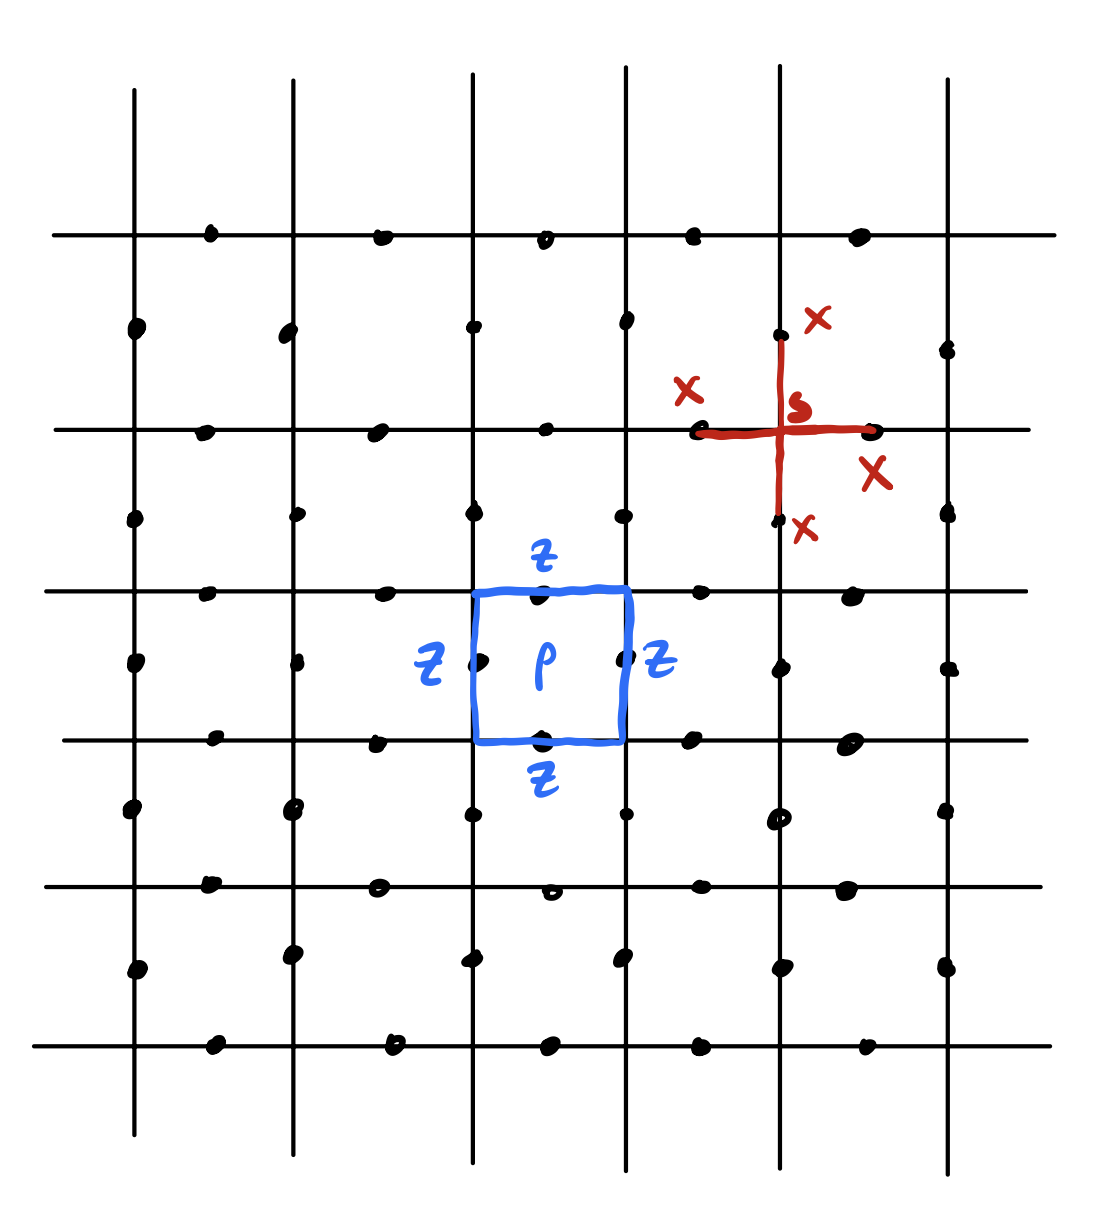
\includegraphics[scale=0.4]{Lectures/Images/lec1-toriccodeops.png}
\end{center}

The $A_s$ term is a product of Pauli-X operators on stars about vertices $s$:
\begin{equation}
    A_s = \prod_{j \in \text{star}(s)} X_j
\end{equation}
And the $B_p$ term is a product of Pauli-$Z$ operators on the boundaries of plaquettes:
\begin{equation}
    B_p = \prod_{j \in \p p}Z_j
\end{equation}
We adopt the QI notation:
\begin{equation}
    X = \sigma^x = \paulix
\end{equation}
\begin{equation}
    Y = \sigma^y = \pauliy
\end{equation}
\begin{equation}
    Z = \sigma^z = \pauliz
\end{equation}'

\subsection{Solving the toric code model}
Notice that all of the $A_s$ and $B_p$ terms commute with one another. For example, its trivial to see that:
\begin{equation}
    [A_s, A_{s'}] = [B_p, B_{p'}] = 0
\end{equation}
because $X$s are mutually commuting and $Z$s are mutually commuting. Slightly less obvious is that the star terms commute with the plaquettes:
\begin{equation}
    [A_s, B_p] = 0
\end{equation}
We might be worried if this holds because $X$ and $Z$ anticommute. But in fact the above holds; if the star and plaquette are faraway then there are no overlapping $X, Z$s so they commute. In the case where the star/plaquette overlap, we have that two $X, Z$s overlap (see picture below) so the anticommutation cancels to a commutation.

\begin{center}
    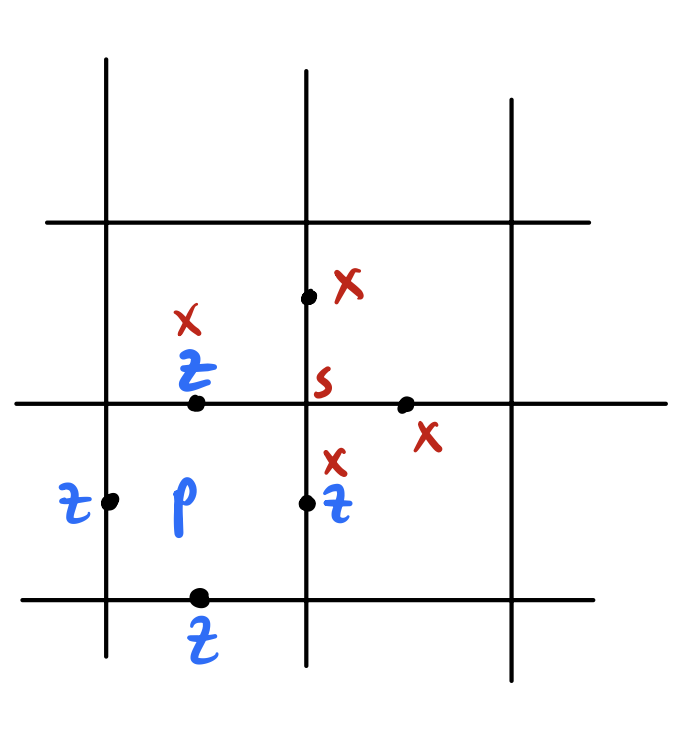
\includegraphics[scale=0.4]{Lectures/Images/lec1-toricopcommute.png}
\end{center}

Thus, we are able to simultaneously diagonalize $\set{A_s, B_p}$. Denote the eigenstates by $\ket{\set{a_s, b_p}}$ where the $a_s, b_p$ are the eigenvalues. If we have residual degeneracy, we may require additional quantum numbers to specify the state, but let us not worry about this quite yet. Note that because:
\begin{equation}
    A_s^2 = B_p^2 = \II
\end{equation}
this implies that the eigenvalues are:
\begin{equation}
    a_s, b_p = \pm 1.
\end{equation}
And the $\ket{set{a_s, b_p}}$ are also the energy eigenstates, with energy:
\begin{equation}
    E = -\sum_s a_s - \sum_p b_p.
\end{equation}
This is the sense in which the problem is exactly solvable. We have found all of the eigenstates, and can find their degeneracies by figuring out the degeneracies of $\set{a_s, b_p}$.

For the ground state, we set $a_s = b_p = 1$. We can ask the question; how many states are there that satisfy this? This is equivalent to asking what the ground state degeneracy is. The answer to this question is dependent on the geometry of the model. Let's start with the simplest, and arguably the most important case; the infinite plane. Let us work in the $X$-basis. In this basis, the different basis states are $\ket{\pm} \otimes \ket{\pm} \otimes \ldots$ for each link. A useful visualization will be in terms of strings on this lattice. In this string picture, we will say that $X_j = -1$ corresponds to a string on link $j$. On the other hand, if $X_j = +1$ then we will say that there is no string on the link. Thus, we can view an arbitrary $X$ basis state as strings occupying the lattice in some configuration.

\begin{center}
    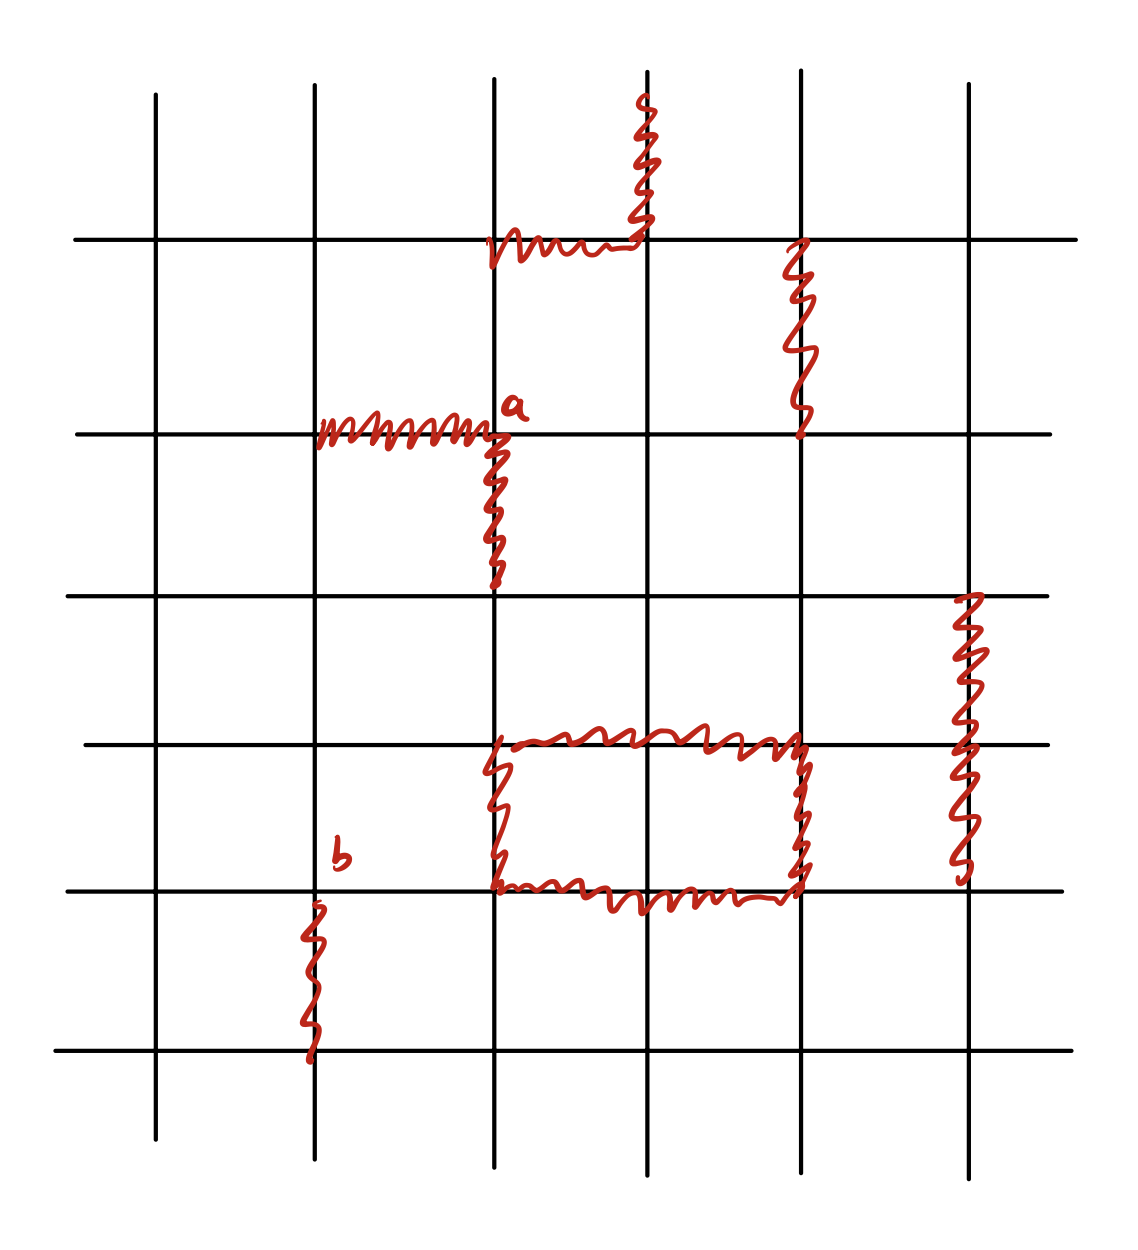
\includegraphics[scale=0.4]{Lectures/Images/lec1-strings.png}
\end{center}

With this point of view, let's figure out what the ground states look like in terms of the $X$-eigenstates. We want $a_s = 1$ for every star, thus $\prod_{j \in \text{star}(s)}X_j = 1$. This implies that the number of -1s in the product must be even. This means that the number of strings that touch a given site must be even. In the above picture, star($a$) obeys this condition while star($b$) does not. But, if $a_s = 1$ for every single star, this implies that the strings must form closed loops (else - at the endpoints of strings we end up with $a_1 = -1$). An allowed configuration is sketched below:

\begin{center}
    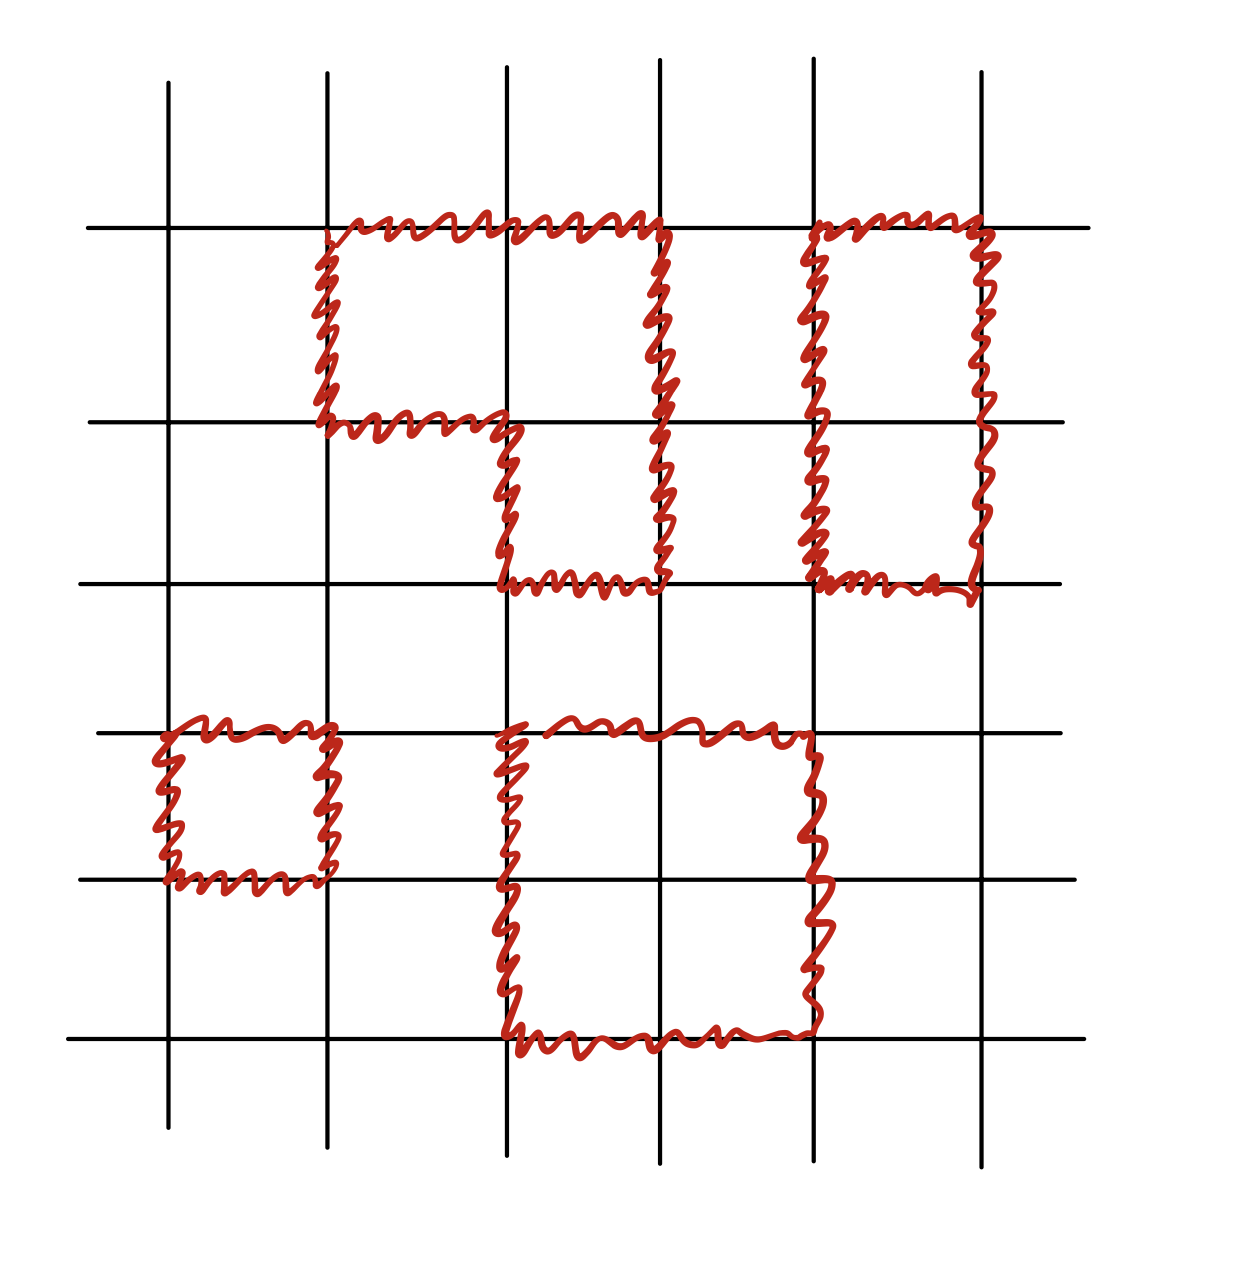
\includegraphics[scale=0.4]{Lectures/Images/lec1-stringsallowed.png}
\end{center}

Note that since $XZ = -ZX$, a given $B_p$ flips string occupation around a plaquette $p$, e.g.:

\begin{center}
    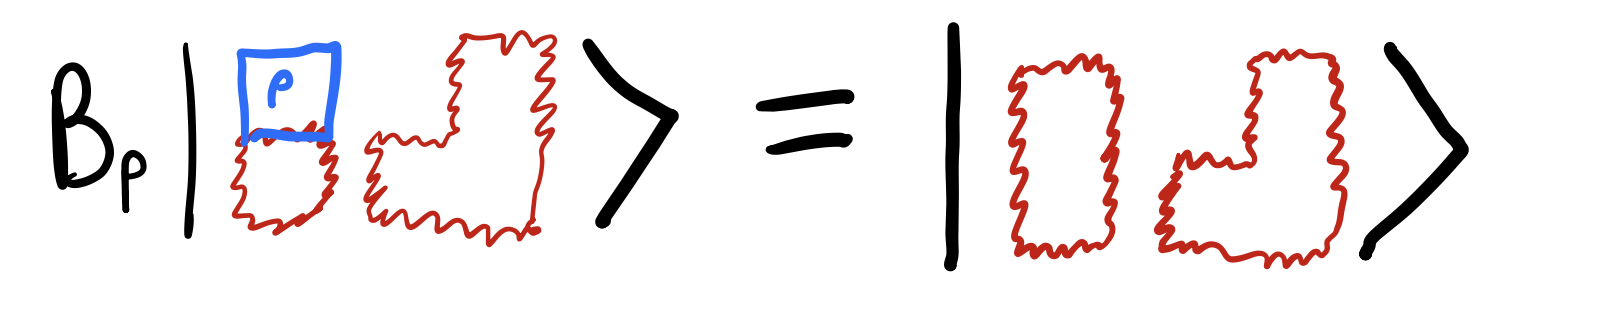
\includegraphics[scale=0.3]{Lectures/Images/lec1-plaquette.png}
\end{center}

But then all of the $a_s = b_p = 1$ requires that we have an equal amplitude superposition of all closed loop states (if this was not the case, the application of some $B_p$ would flip some loops and change the state - not an eigenstate!). Thus! There is a unique ground state:
\begin{equation}
    \ket{\Omega} = \ket{a_s = b_p = 1} = \sum_{\text{closed loop config $C$}}\ket{C}.
\end{equation}
We could draw an example $\ket{C}$ pictorially as:
\begin{center}
    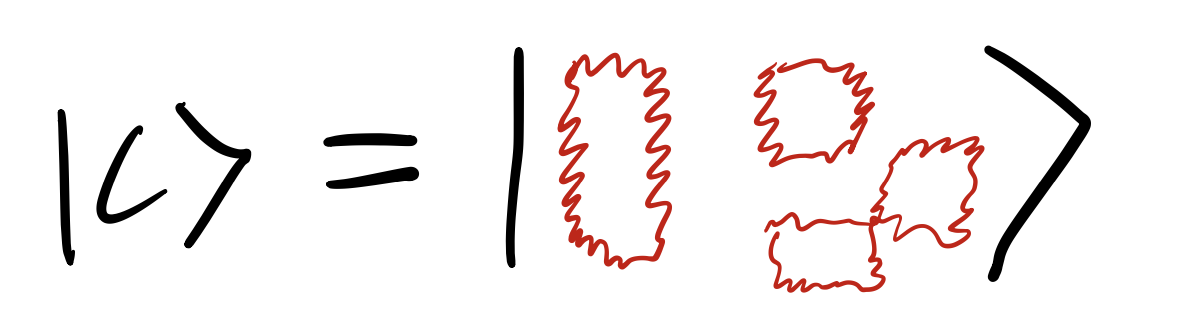
\includegraphics[scale=0.3]{Lectures/Images/lec1-closedloop.png}
\end{center}
It can be seen that $B_p$ only permutes the different $C$s to each other without changing their weight, so indeed the above is the $+1$ eigenstate of the $B_p$s. More formally, if $B_p\ket{\psi} = \ket{\psi}$ for all $p$, then:
\begin{equation}
    \braket{C}{\psi} = \bra{C}B_p\ket{\psi} = \braket{C'}{\psi}
\end{equation}
where $\ket{C'}$ is a different closed loop configuration. This implies that all of the amplitudes of the closed loop configurations have equal weight.

Note that formally there is an infinite number of closed loop configurations on an infinite plane, so there is a bit of a subtlety in normalizing the state (which requires the machinery of operator algebras, etc.) which we sweep under the rug.

Note that the above argument gave a unique state for $a_s = b_p = 1$, but for any choice of $\set{a_s, b_p}$ we can get a statement of a similar flavour. Thus, this justifies the choice of notation $\ket{\set{a_s, b_p}}$ as for a given choice of $a_s/b_p$ the state is unique.

Now, we have the full energy spectrum, as we have determined the degeneracy of all of the eigenspaces. We can thus determine the energy gap, which is the energy difference between the ground state and first excited state. Flipping one of the $a_s$ or the $b_p$ results in an energy penalty of $2$, and thus the energy gap is $\Delta = 2$. This is important because it means that we have a ``gapped Hamiltonian''. In comparison, there are ``gapless'' Hamiltonians for which the energy difference goes to zero in the thermodynamic limit. This distinction/property will be important when we discuss anyons - gapped Hamiltonians are the context in which they are currently understood.

\subsection{Excitations and String Operators}
There are two types of elementary excitations:
\begin{enumerate}
    \item $a_s = -1$ for some $s$; this is a ``charge'', and lives on a site.
    \item $b_p = -1$ for some $p$; this is a ``flux'', and lives on a plaquette.
\end{enumerate}
\begin{center}
    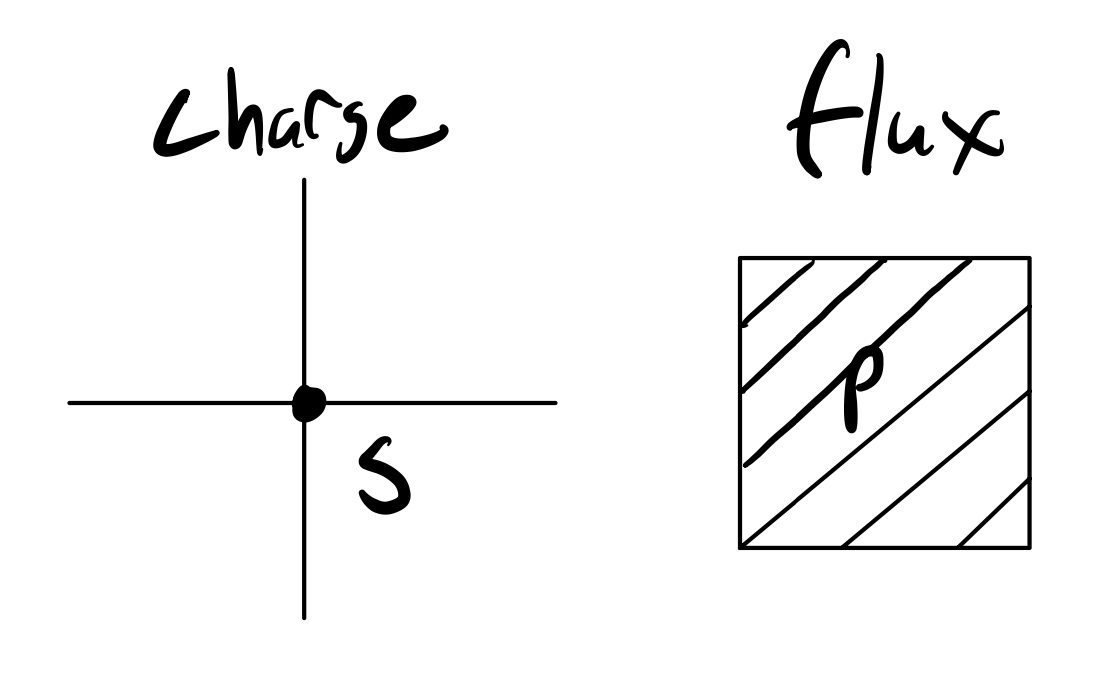
\includegraphics[scale=0.4]{Lectures/Images/lec1-excitations.png}
\end{center}
The terminology comes from $\ZZ_2$ gauge theory. We will see that these excitations are not conventional bosons or fermions that we may be familiar with.

If we visualize these excitations, adding a charge is like taking our superposition of all closed loops and then to each of those states adding one defect (with a string that goes off to infinity). Adding a plaquette takes the superposition of loops, and we count the number of loops that go around $p$ (a kind of winding number) and take that to be the sign of the configuration in the superposition. Pictorially, we have defects in the first case and vortices in the second.

Now, the question becomes how can we create charge or flux excitations? In spin systems you might be familiar with (e.g. creating a magnon in a Heisenberg spin chain) you would create them via a local operator. But here we actually apply a non-local string operator to create these excitations.

We define:
\begin{equation}
    W^Z(\gamma) = \prod_{j \in \gamma}Z_j
\end{equation}
where $\gamma$ is some open path on the lattice. The $W^Z(\gamma)$ is a string of $Z$s along $\gamma$. This string operator creates charge excitations at the two endpoints; notice that:
\begin{equation}
    [W^Z(\gamma), B_p] = 0
\end{equation}
this is obvious as the $B_p$s consist of $Z$s only. Less obvious is that the $W^Z(\gamma)$ commutes with almost all of the $A_s$ operators - all except at the endpoints of $\gamma$, $s_1$ and $s_2$. 

\begin{center}
    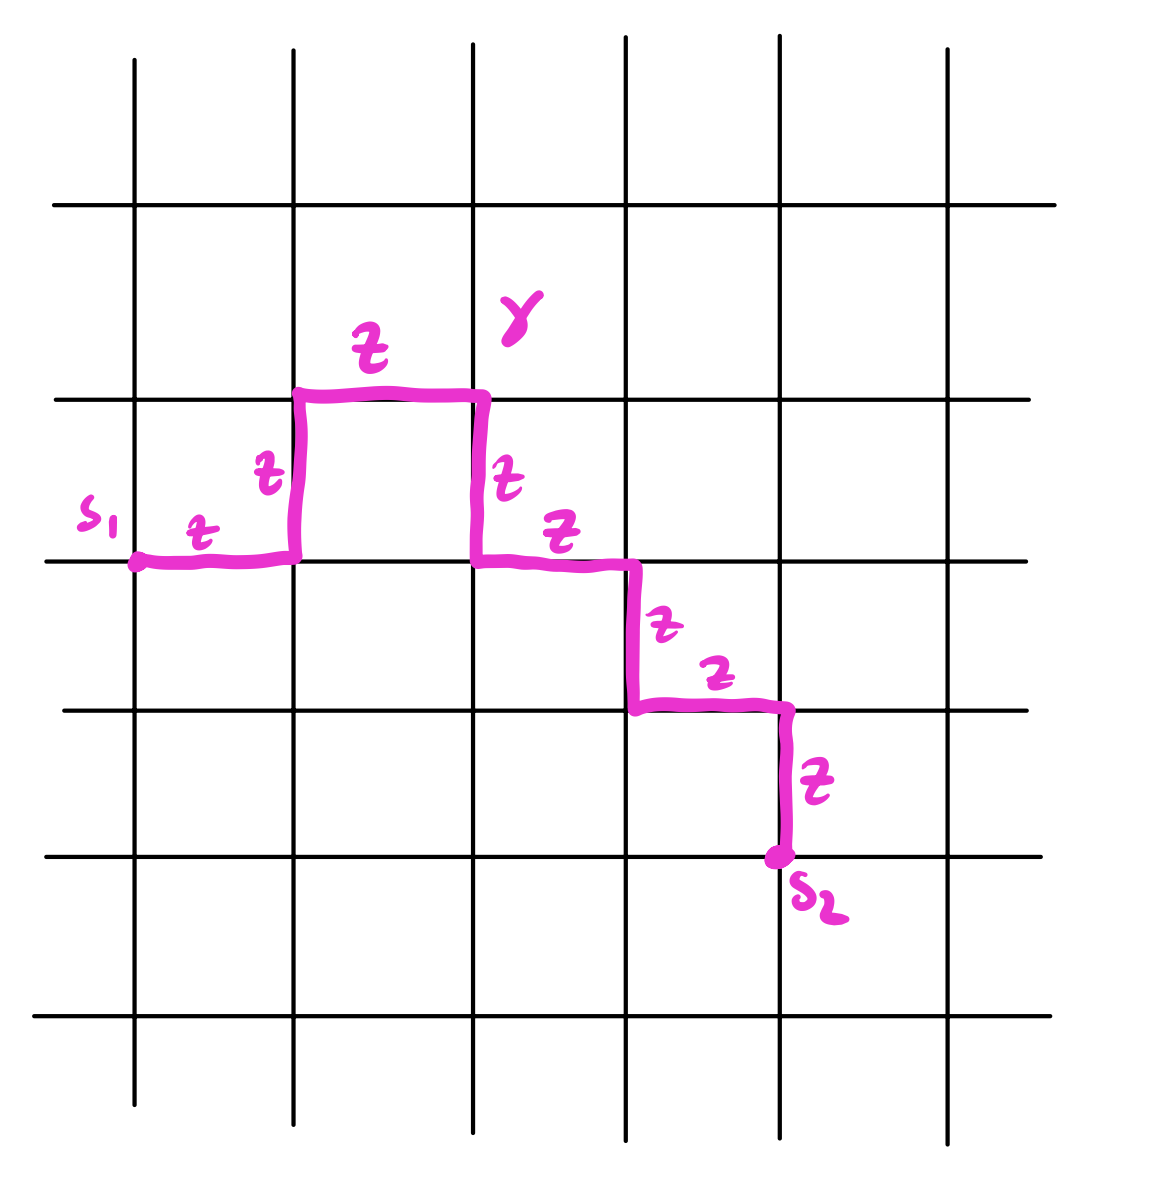
\includegraphics[scale=0.4]{Lectures/Images/lec1-stringop.png}
\end{center}

Let us argue this. At intermediate points along the path each of the points have an even number of strings so we have commutation. At the endpoints, we only have 1 link and so we have anticommutation:
\begin{equation}
    W^Z(\gamma)A_{s_{1,2}}  = -A_{s_{1,2}}W^z(\gamma)
\end{equation}
What are the implications of this? Looking at the ground state $\ket{\Omega} = \ket{\set{a_s=b_p=1}}$:
\begin{equation}
    W^Z(\gamma)\ket{\Omega} = \ket{\set{a_{s_1} = a_{s_2} = -1, \text{others} = 1}}.
\end{equation}
and we can see this because the string operator only flips the stars at the endpoints, and commutes with everything else. Thus, we conclude that the $W^Z(\gamma)$ creates charges at the two endpoints of $\gamma$, as claimed.

An important observation with regard to string operators; If $\gamma'$ is a different path with the same endpoints, then the string operator $W^z(\gamma')$ applied to the ground state yields the \emph{exact} same state (even up to the same phase):
\begin{equation}
    W^Z(\gamma)\ket{\Omega} = W^z(\gamma')\ket{\Omega}
\end{equation}
this is the notion in which string operators are ``flexible''. To see this, note that $W^Z(\gamma') = W^Z(\gamma)\prod_{p \in \text{int}(\gamma' \cup \gamma)}B_p$, i.e. the two operators are related via a product of plaquette operators in the interior of the two paths. Thus:
\begin{equation}
    W^Z(\gamma')\ket{\Omega} = W^z(\gamma)\prod_{p \in \text{int}(\gamma' \cup \gamma)}B_p\ket{\Omega} = W^Z(\gamma)\ket{\Omega}
\end{equation}
where we have used that $\ket{\Omega}$ is the $+1$-eigenstate of all the $B_p$s.

\begin{center}
    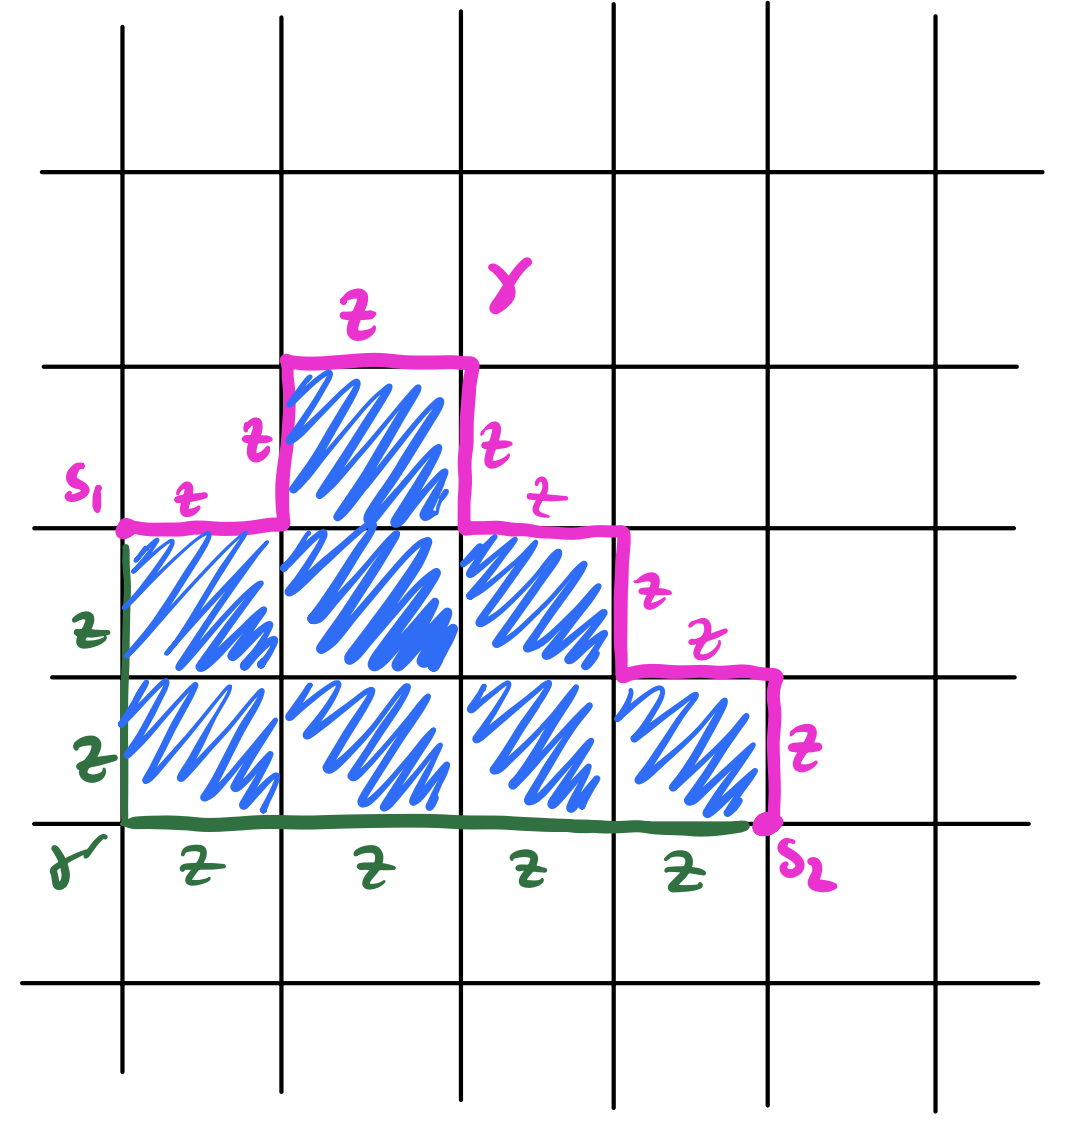
\includegraphics[scale=0.4]{Lectures/Images/lec1-flexible.png}
\end{center}

Relatedly, if $\gamma$ is a closed loop then:
\begin{equation}
    W^Z(\gamma)\ket{\Omega} = \ket{\Omega}
\end{equation}
which follows from the fact that a closed loop is just a product of $B_p$s.

\begin{center}
    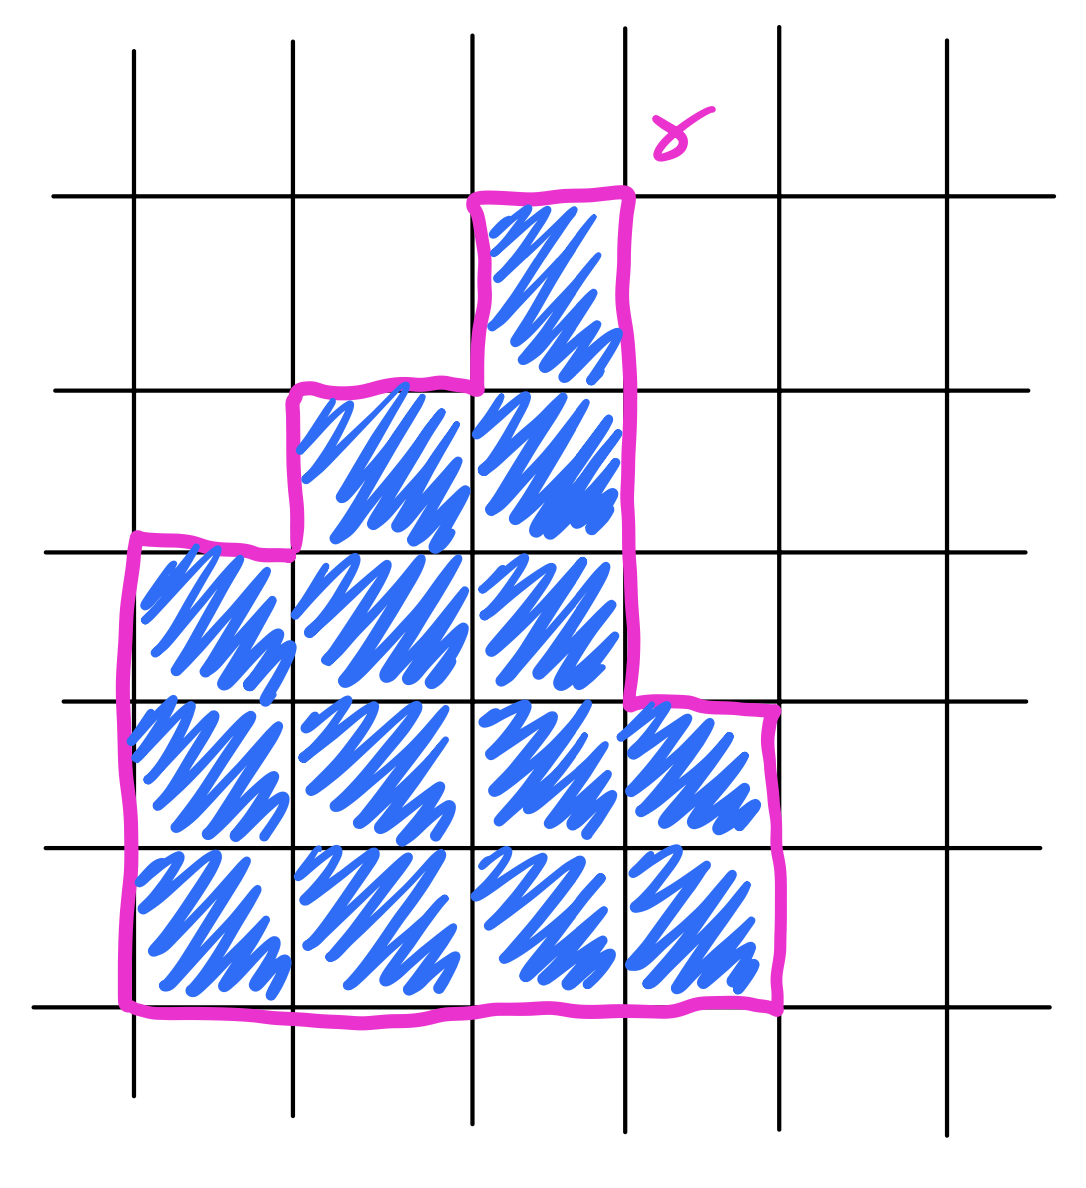
\includegraphics[scale=0.4]{Lectures/Images/lec1-loopstringop.png}
\end{center}


These features - which currently seem pretty specific to the toric code model - are in fact quite general. Any system with anyons have string operators with these properties!

A last comment to provide some physical intuition for what the string operator is. We can view it as the physical process of first creating two charges (by applying a single $Z$), then moving that charge via the application of further $Z$s along the path. I.e. a string operator is just creating two charges and separating them. This makes the notion that the string is flexible intuitive; we should get the same state (up to some phase) if the particles are created and end up in some separated location(s), no matter how we move them there.
\section{Toric Code II}
\subsection{Review}
A quick review of some definitions; the Toric code has Hamiltonian (defined on a 2D lattice with qubits placed on the edges):
\begin{equation}
    H = - \sum_s A_s - \sum_p B_p
\end{equation}
with $A_s$ star operators around each lattice vertex:
\begin{equation}
    A_s = \prod_{j \in \text{star}(s)}X_s
\end{equation}
and $B_p$ plaquette operators around each lattice plaquette
\begin{equation}
    B_p = \prod_{j \in \partial p}Z_p
\end{equation}
we constructed the ground state $\ket{\Omega} = \ket{a_s = b_p = 1}$. We also discussed a string operator, which creates charge excitations:
\begin{equation}
    W^Z(\gamma) = \prod_{j \in \gamma}Z_j
\end{equation}
where $\gamma$ is a path on the lattice. It creates charges ($a_s = -1$) at the endpoints of $\gamma$. Further, these string operators are flexible, in the sense that:
\begin{equation}
    W^Z(\gamma)\ket{\Omega} = W^Z(\gamma')\ket{\Omega}
\end{equation}
for two paths $\gamma, \gamma'$ with the same endpoints.

\subsection{String operator for flux excitations}
There is a similar string operator for flux excitations. Just a heads up that the structure of having string operators (one for each anyon type - here for charges and fluxes/$e$ and $m$) is quite general. We define:
\begin{equation}
    W^X(\hat{\gamma}) = \prod_{j \in \hat{\gamma}}X_j
\end{equation}
where $\hat{\gamma}$ is an open path on the dual lattice, i.e. that go through the center of plaquettes:

\begin{center}
    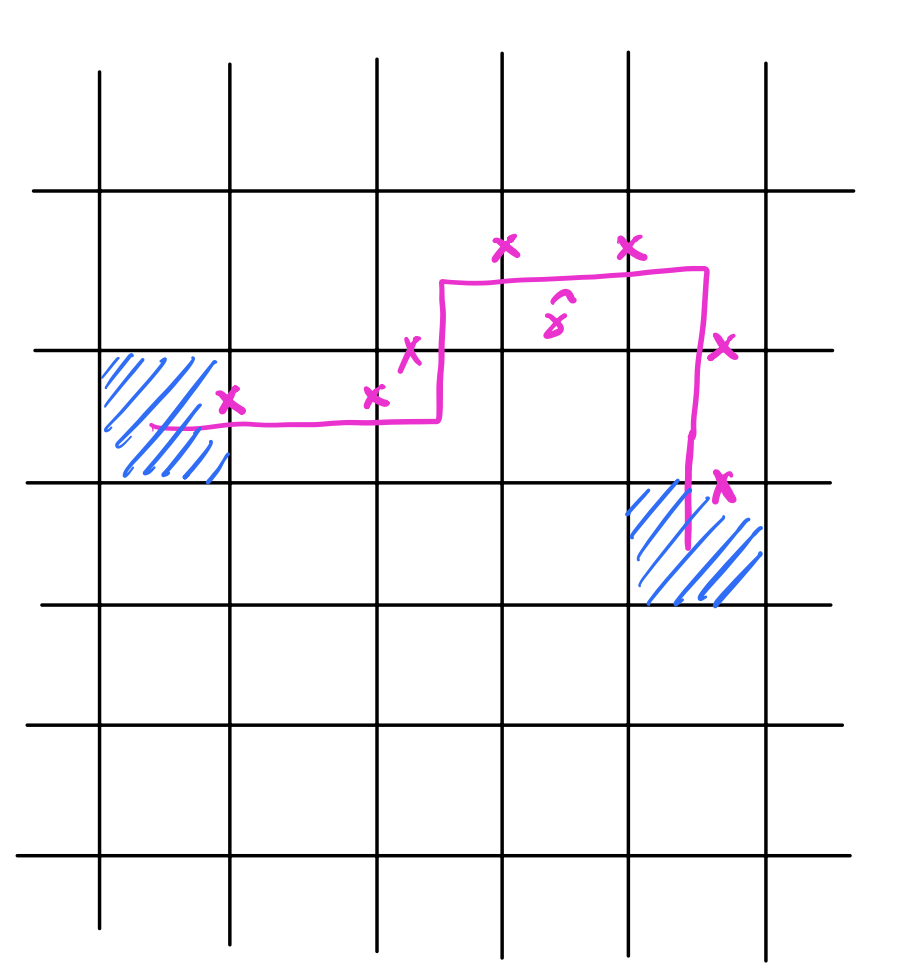
\includegraphics[scale=0.4]{Lectures/Images/lec2-fluxstring.png}
\end{center}

Much like the string operator for the charges:
\begin{itemize}
    \item It can be checked that $W^X(\hat{\gamma})$ creates fluxes $b_p = -1$ at the two endpoints of $\hat{\gamma}$.
    \item The string operators are flexible, with:
    \begin{equation}
        W^X(\hat{\gamma})\ket{\Omega} = W^X(\hat{\gamma}')\ket{\Omega}
    \end{equation}
    for $\hat{\gamma}, \hat{\gamma}'$ with the same endpoints. They are related by the product of star operators on the interior.
    \begin{center}
        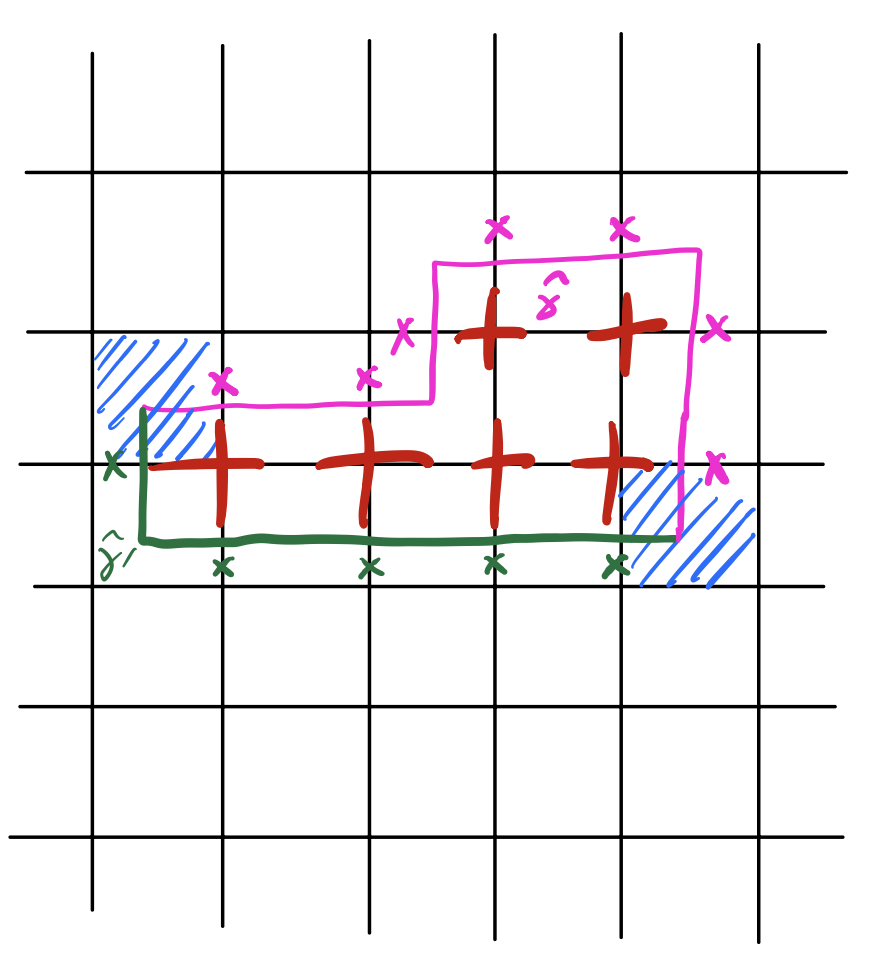
\includegraphics[scale=0.4]{Lectures/Images/lec2-fluxstring2.png}
    \end{center}
\end{itemize}

The existence of these flexible, non-commuting string operators is very fundamental to the structure of the toric code, and to anyon systems more generally. The existence of these is independent of geometries. But we will see that it will have implications when we consider the model for specific systems.

\subsection{Ground state degeneracy on a torus}
\begin{center}
    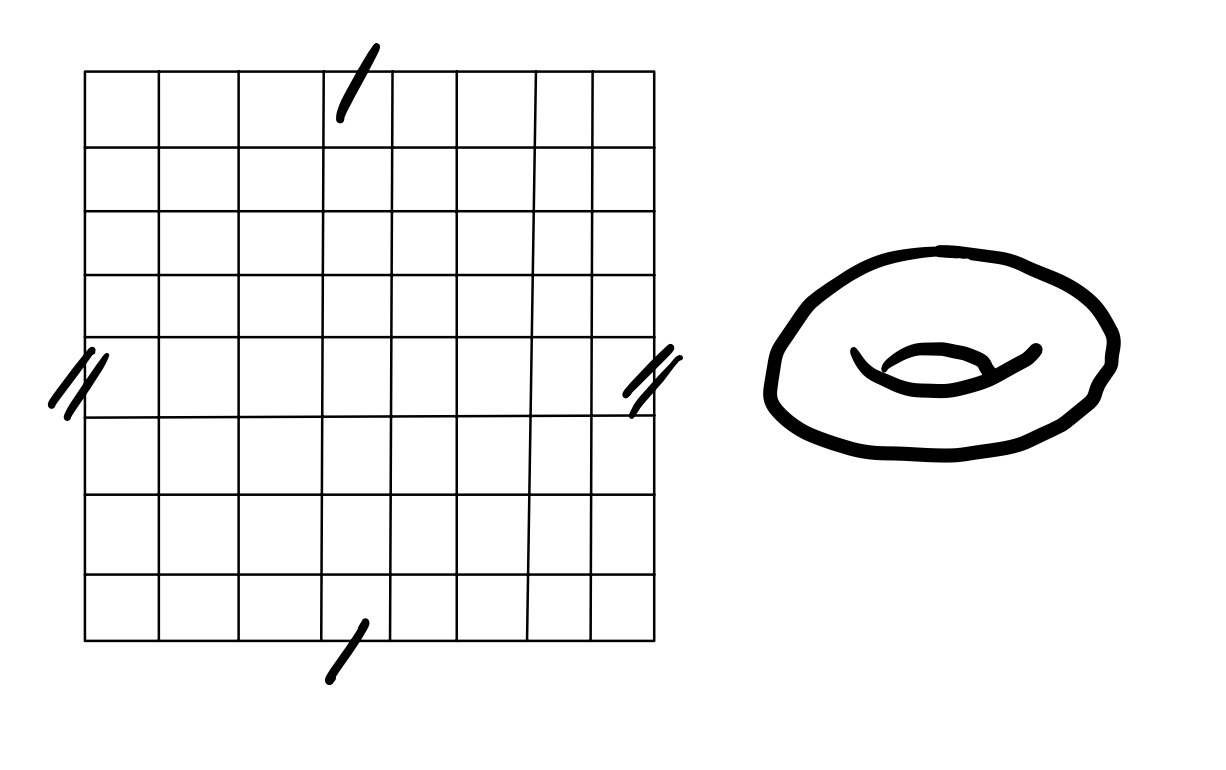
\includegraphics[scale=0.4]{Lectures/Images/lec2-torus.png}
\end{center}
Consider the toric code, on a finite ($L \times L$) torus. We may have different allowable states for a given $a_s$ and $b_p$, and thus may find that there are different degeneracies, compared to the infinite plane case.  We can now ask what is the ground state degeneracy $D$? Indeed, this question is equivalent to asking what the dimension of the eigenspace with $a_s = b_p = 1$ is. To find this, we look at the trace of the projector onto the eigenspace\footnote{This is a very formal way to find it, we will soon get different perspectives on this question}:
\begin{equation}
    \begin{split}
        D &= \Tr(\text{proj. onto $a_s = b_p = 1$ subspace})
        \\ &= \Tr(\prod_{s}\left(\frac{\II + A_s}{2}\right)\prod_{p}\left(\frac{\II + B_p}{2}\right))
    \end{split}
\end{equation}
where the second line follows from the fact that the product of the (mutually commuting) projectors gives the projector onto the subspace. Computing this:
\begin{equation}
    D = \frac{1}{2^{N_s}}\frac{1}{2^{N_p}}\Tr(\prod_{s}(\II + A_s)\prod_{p}(\II + B_p))
\end{equation}
Now we expand out this product, and can think about the traces of the individual terms. A single $A_s, B_p$ will be traceless (as the Paulis are traceless), and so will most products of $A_s, B_p$; the only non-traceless terms will be those that simplify to the identity. If we stare at this, there are only a few combinations for which this occurs; there is the term with all identity, the term with all stars (all the $X$s cancel), the term with all plaquettes (all the $Z$s cancel), and the term with all stars and all plaquettes.
\begin{equation}
    D = \frac{1}{2^{N_s}}\frac{1}{2^{N_p}}\Tr(\II + \prod_s A_s + \prod_p B_p + \prod_s\prod_p A_sB_p) = \frac{1}{2^{N_s}}\frac{1}{2^{N_p}}\Tr(4\II)
\end{equation}
Now looking at the trace of the identity:
\begin{equation}
    \Tr(\II) = 2^{\text{dim}(\mathcal{H})} = 2^{N_{\text{links}}}
\end{equation}
Thus:
\begin{equation}
    D = \frac{1}{2^{L^2}}\cdot \frac{1}{2^{L^2}} \cdot 4 \cdot 2^{2L^2} = 4
\end{equation}
so:
\begin{equation}
    \boxed{D = 4}
\end{equation}
A nice feature of this argument is we can repeat it for any of the eigenspaces. In fact, every $\set{a_s, b_p}$ eigenspace with $\prod_s a_s = \prod_p b_p = 1$ (i.e. an even number of charges) is 4-fold degenerate. 

\subsection{Ground states in the string picture}

Now, let's see if we can understand the ground state degeneracy in the string picture. To review, we work in the $X$-basis, and $X_j = \pm 1$ corresponds to there being a string (plus) or no string on link $j$. $a_s = 1$ requires the product of $X$s on the star to be one, implying that the strings form closed loops. $b_p = 1$  implies that there is an equal amplitude superposition of string states, as different string states are related by $B_p$ moves. We used these two conditions on the infinite plane geometry (Where $B_p$ moves are ``ergodic'') to say that there was a unique ground state, namely that with an equal weight superposition of all closed loop configurations:
\begin{equation}
    \ket{\Omega} = \sum_{\text{closed loop config $C$}}\ket{C}
\end{equation}
On a torus, the closed loop states can be divided into 4 classes; even/even, even/odd, odd/even, and odd/odd. 

\begin{center}
    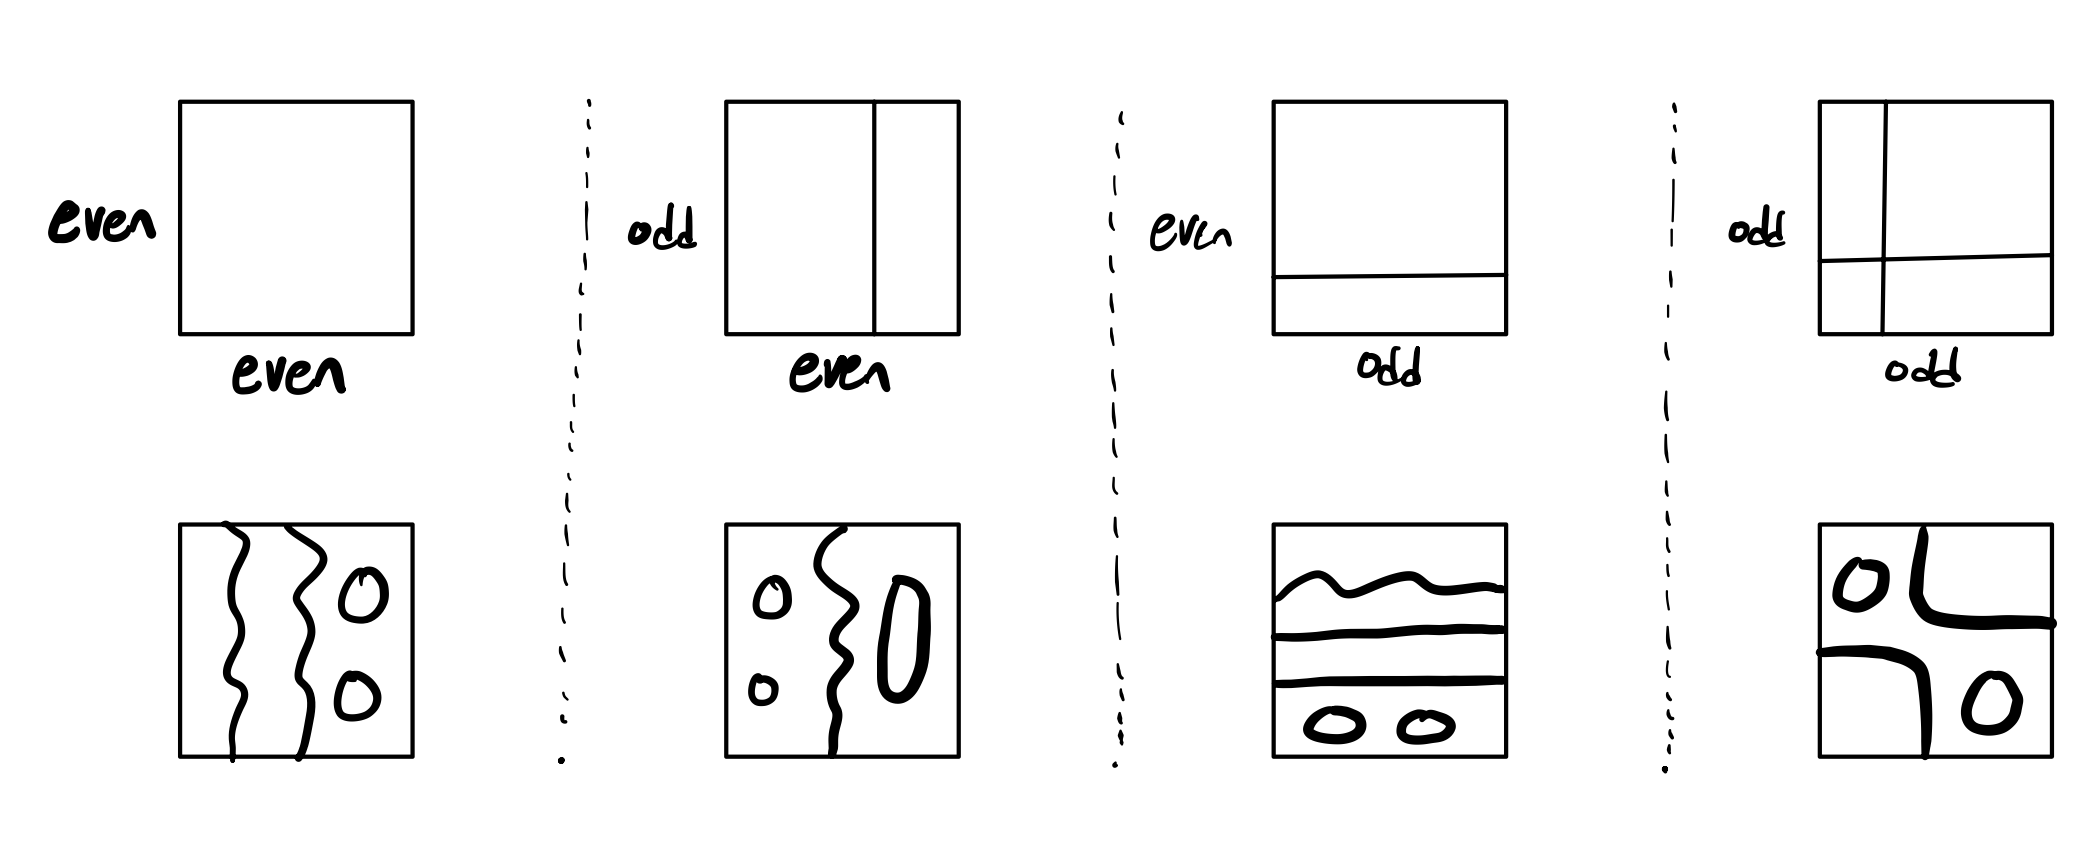
\includegraphics[scale=0.4]{Lectures/Images/lec2-evenodd.png}
\end{center}

What does this mean? this means that if we draw a line going across the torus (on the dual lattice), we ``cross'' an even/odd number of strings. Within each sector/class, the $B_p$ moves are ergodic. But, $B_p$ moves cannot change the parity of the crossings. Thus the four degenerate ground states correspond to the equal weight superpositions of closed loop configurations within a given class. We can label the ground states via their winding number:
\begin{equation}
    \ket{\Omega_{(e/o, e/o)}} = \sum_{\text{closed loop config $C$ with (e/o, e/o) winding}}\ket{C}
\end{equation}

So, so far we have understood the ground state degeneracy from two perspectives. But neither of these tells us the deeper principle underlying the degeneracy. Let us discuss this now - it will allow us to see why the degeneracy is topologically protected.

\subsection{Origin of the ground state degeneracy}
The punchline is that the GSD comes from the existence of non-commuting string operators.

Define the charge string operators:
\begin{equation}
    W_1^Z = \prod_{j \in \gamma_1}Z_j
\end{equation}
\begin{equation}
    W_2^Z = \prod_{j \in \gamma_2}Z_j
\end{equation}
These string operators correspond to the creation and subsequent annihilation of a charge as the string wraps around the torus. We can also define the string operators for the fluxes;
\begin{equation}
    W_1^X = \prod_{j \in \hat{\gamma}_1}X_j
\end{equation}
\begin{equation}
    W_2^X = \prod_{j \in \hat{\gamma}_2}X_j
\end{equation}

\begin{center}
    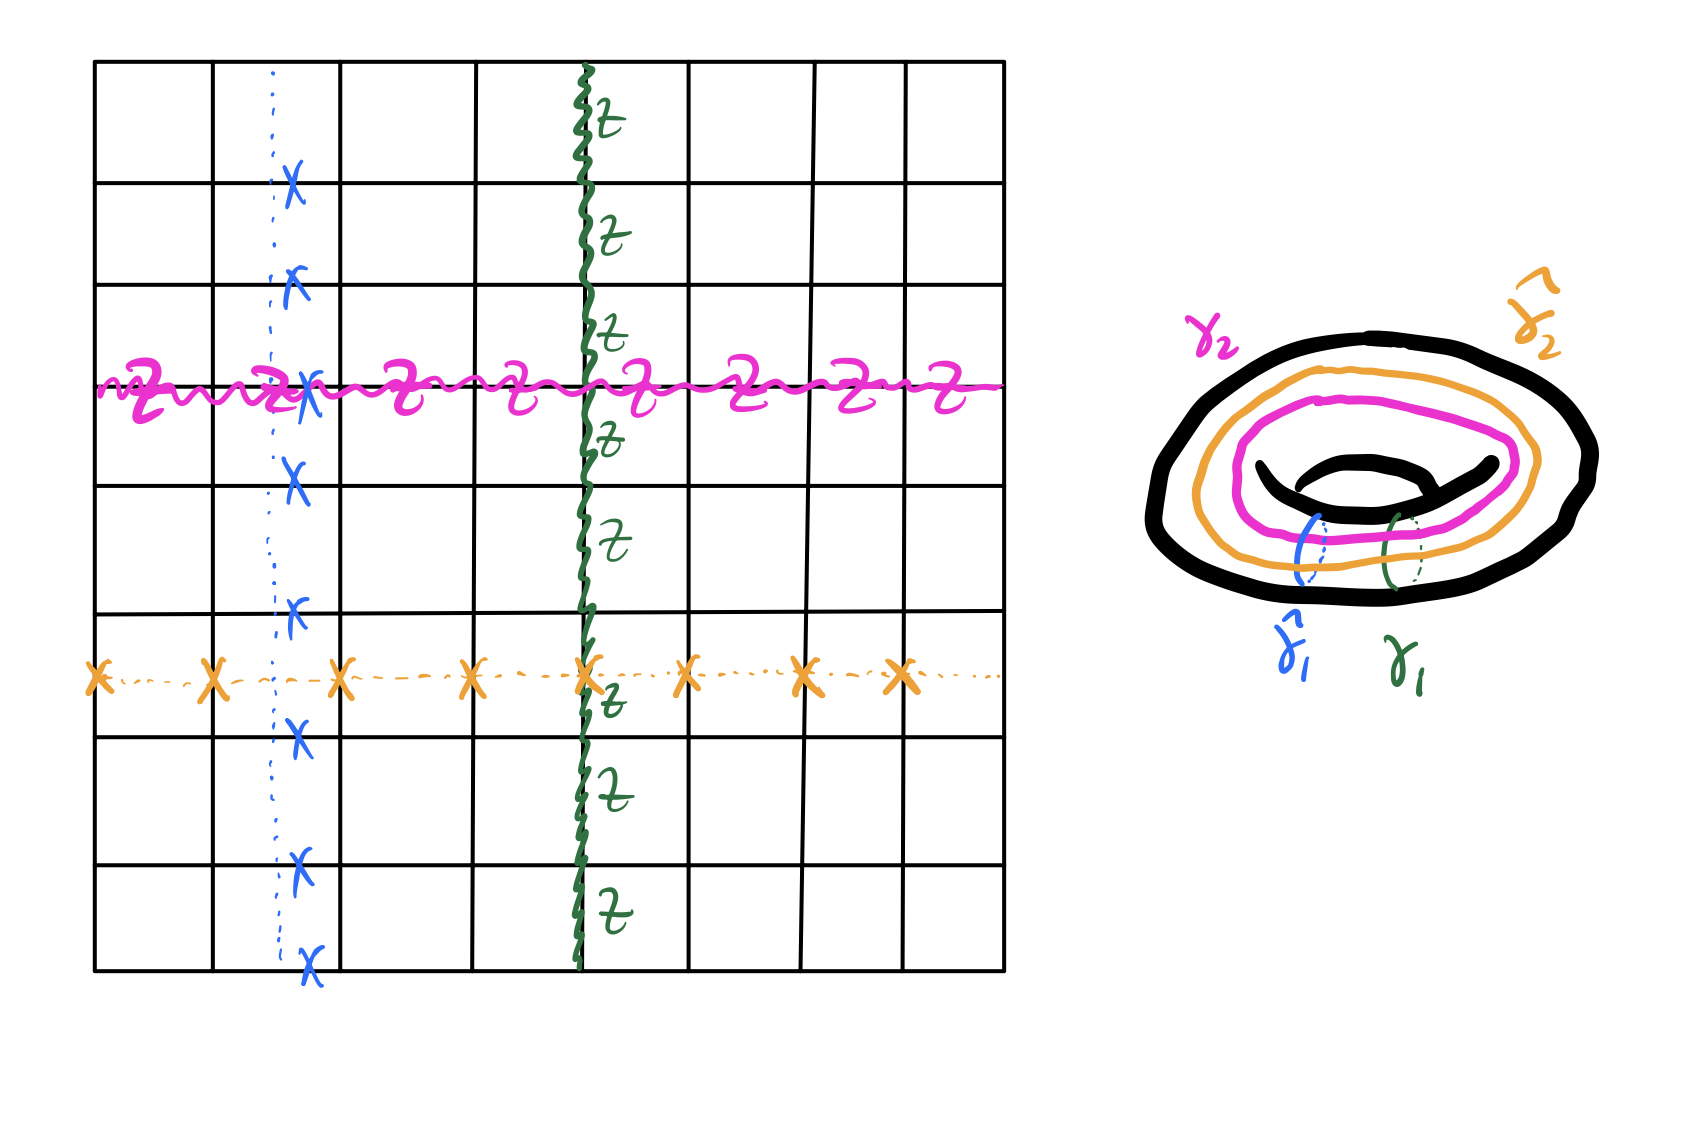
\includegraphics[scale=0.4]{Lectures/Images/lec2-torusstrings.png}
\end{center}

Notice that:
\begin{equation}
    \begin{split}
        [W_i^Z, A_s] &= [W_i^Z, B_p] = 0
        \\ [W_i^X, A_s] &= [W_i^X, B_p] = 0
    \end{split}
\end{equation}
so they map ground states to ground states. They have an interesting commutation algebra. $\set{W_1^Z, W_2^Z, W_1^X, W_2^X}$ all commute, except for two exceptions:
\begin{equation}
    \begin{split}
        W_1^XW_2^Z &=  -W_2^ZW_1^X
        \\ W_2^XW_1^Z &=  -W_1^ZW_2^X
    \end{split}
\end{equation}
this is because they anticommute in one place.

\begin{center}
    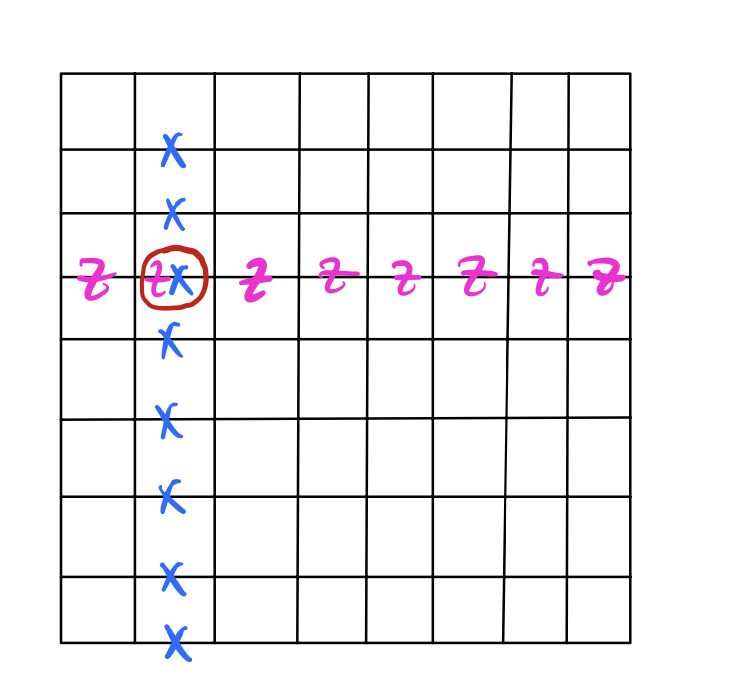
\includegraphics[scale=0.4]{Lectures/Images/lec2-torusanticommute.png}
\end{center}

The fact that the other commute is clear; the fact that the $X$s mutually commute and $Z$s mutually commute is immediate. For $W_1^X, W_1^Z$, they act on disjoint regions. Even if you were to pick representatives that overlap, they will overlap an even amount of times.

\begin{center}
    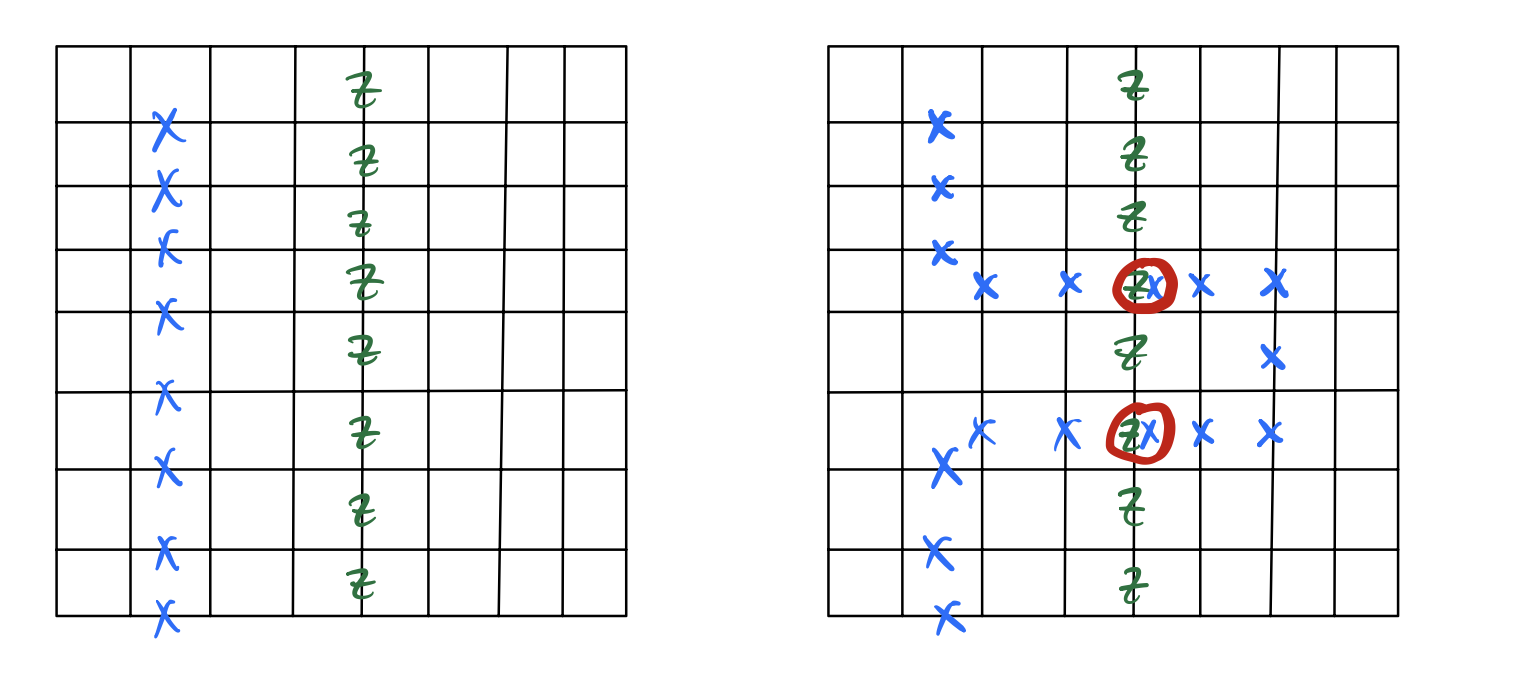
\includegraphics[scale=0.4]{Lectures/Images/lec2-toruscommute.png}
\end{center}

This algebra is quite interesting; we have symmetry generators that commute with the Hamiltonian, but not with each other. A simple HW exercise you will do is that the eigenstates/ground states will come in multiplets of 4 (the fact that it is exactly 4 in this case comes from the microscopic calculation).

A final comment; we said how the $\set{a_s, b_p}$ do not uniquely specify the ground (or excited) states. But in fact the string operators provide the missing quantum numbers necessary to specify the state. Specifically, we can uniquely label the eigenstates by choosing (in addition to the $\set{a_s, b_p}$) the values of the $W$s, e.g $\ket{\set{a_s, b_p}, w_1^x, w_2^x}$ where $w_1^x = \pm 1$ and $w_2^x = \pm 1$. We can thus denote the four ground states as $\ket{\Omega, \pm\pm}$. These are \emph{exactly} the same what we called before the $\ket{\Omega_{(e/o, e/o)}}$ - in fact the $W^x$ string operator counts the number of crossing of $X$ strings.

Next time, we will discuss how the GSD is robust to arbitrary local perturbations - it is topologically protected.
\section{Toric Code III, Berry Phase}

\subsection{Robustness of toric code GSD}
We saw the degeneracy of the toric code from both the explicit/formal calculation as well as from string operators. GSD in itself is not interesting, and is quite fragile; perturbations tend to split it - what is interesting about the TC GSD is that it is extremely robust; local perturbations cannot split it.

More precisely, consider an arbitrary local perturbation of $H$:
\begin{equation}
    H' = H + \lambda\sum_j V_j
\end{equation}
where $V_j$ is a local operator supported near site $j$.

\begin{center}
    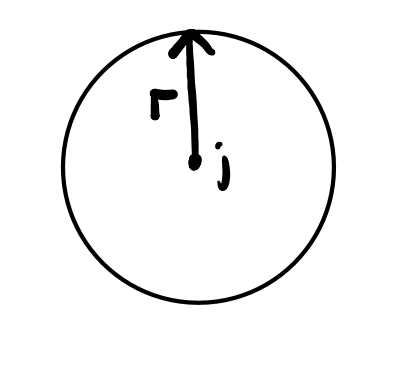
\includegraphics[scale=0.4]{Lectures/Images/lec3-local.png}
\end{center}

Claim: For sufficiently small $\lambda$, $H'$ has 4 nearly degenerate ground states with splitting:
\begin{equation}
    \delta \leq e^{-\text{C}(\lambda)L} 
\end{equation}
with $C(\lambda)$ a $\lambda$-dependent constant. The idea is that with a arbitrary local perturbation we have an exponentially small (in the thermodynamic limit) splitting of the ground state manifold, and thus the GSD is robust. From a QI perspective, this is useful because it tells us that we have a robust encoding of a qubit - we can use the ground state as a robust subspace. This degeneracy is often called a ``protected'', or topological because it is automatically protected.

\begin{center}
    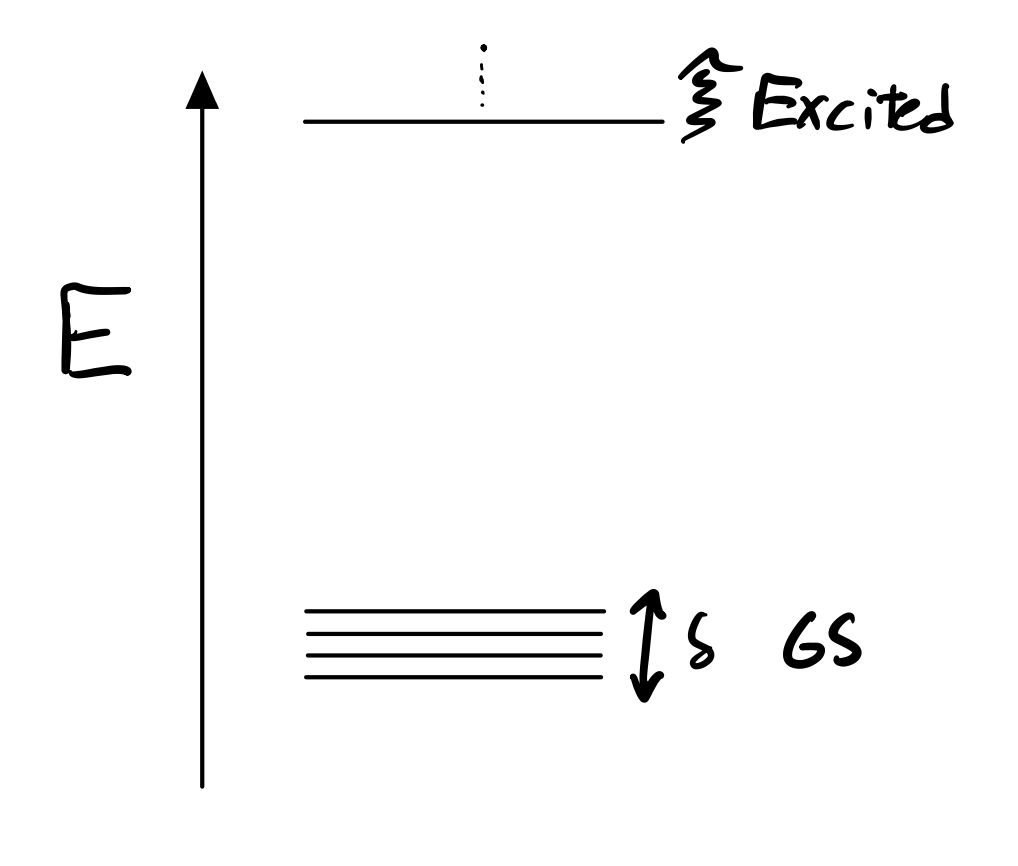
\includegraphics[scale=0.3]{Lectures/Images/lec3-gsmanifold.png}
\end{center}

\subsection{Argument for robustness}
Using the fact that $\set{W_1^X, W_2^X, W_1^Z, W_2^Z}$ (string operators) are flexible and non-commuting, we can establish a key property of the unperturbed ground states $\ket{\Omega, \pm}$. Namely, for any operator $O$ supported on less than $L$ sites:
\begin{equation}\label{eq:star}
    \bra{\Omega, \pm, \pm}O\ket{\Omega, \pm, \pm} = \text{diag}(c, c, c, c)
\end{equation}
for some constant $c$. A shorthand for the above is:
\begin{equation}
    \bra{\Omega, \alpha}O\ket{\Omega, \beta} = c\delta_{\alpha\beta}.
\end{equation}
You will show this relation on the homework.

Let's unpack this equation. The first thing it tells us is that:
\begin{equation}
    \bra{\Omega, \alpha}O\ket{\Omega, \alpha} = \bra{\Omega, \alpha'}O\ket{\Omega, \alpha'}
\end{equation}
which tells us that local operators cannot distinguish different ground states. The second thing it tells us is that:
\begin{equation}
    \bra{\Omega, \alpha'}O\ket{\Omega, \alpha} = 0 \quad \text{for }\alpha \neq \alpha'
\end{equation}
in other words, local operators cannot connect ground states.

As a comparison, consider $\ket{\uparrow}^{\otimes N}, \ket{\downarrow}^{\otimes N}$ the 2-fold degenerate ground states of the Ising model $H = -\sum_{ij}Z_iZ_j$. A local operator cannot connect them, but it is possible to distinguish the two states by measuring $Z_i$. In a symmetry breaking state, we do not have the structure of flexible strings, and hence do not have the same notion of local indistinguishability to arbitrary operators (only to symmetric ones).

Using the local distinguishability/unconnectability, let us sketch an argument for the toric code GSD. For concreteness, consider a perturbation:
\begin{equation}
    H' = H + \lambda \sum_j X_j.
\end{equation}
To obtain the first-order splitting (in degenerate perturbation theory), we need to find the matrix elements:
\begin{equation}
    \bra{\Omega, \pm, \pm}\sum_j X_j\ket{\Omega, \pm, \pm}
\end{equation}
and then diagonalize. By Eq. \eqref{eq:star}, we know that:
\begin{equation}
    \bra{\Omega, \pm, \pm}X_j\ket{\Omega, \pm, \pm} = c_j\II
\end{equation}
Therefore the ground state degeneracy is not split to first order. Looking at second order, we need to find matrix elements:
\begin{equation}
    \bra{\Omega, \pm, \pm}(\sum_j X_j)(H-E_{\text{gs}})^{-1}\Pi_{\text{ex}}(\sum_j X_j)\ket{\Omega, \pm, \pm}
\end{equation}
and then diagonalize (third, fourth order (and so on) we have the same procedure, just add a factor of $(H-E_{\text{gs}})^{-1}\Pi_{\text{ex}}(\sum_j X_j)$ each order). A given $X_j$ takes us to an excited state, the $\Pi_{\text{ex}}$ projector is then irrelevant\footnote{For a general operator, we instead can use that the projector can be restricted to a local operator as we only need to look at some local patch to tell that we are in an excited state}, and then $(H-E_{\text{gs}})^{-1}$ is just a number (difference between the ground and excited state energy), so we end up evaluating matrix elements of the form:
\begin{equation}
    \bra{\Omega, \pm, \pm}X_j X_k\ket{\Omega, \pm, \pm} = c\II
\end{equation}
where we again use Eq. \eqref{eq:star}. So, again at second order we have no splitting, and the argument follows the same way for third, fourth order etc. using the same property. The argument only breaks when the property no longer holds, which occurs at $L$th order of perturbation theory when we end up looking at the matrix element of an operator supported on $L$ sites. In particular, we get terms of the form:
\begin{equation}
    \prod_{j\in\hat{\gamma}_1}X_j = W_1^X, \quad \prod_{j\in\hat{\gamma}_2}X_j = W_2^X
\end{equation}
i.e. the string operators.

\begin{center}
    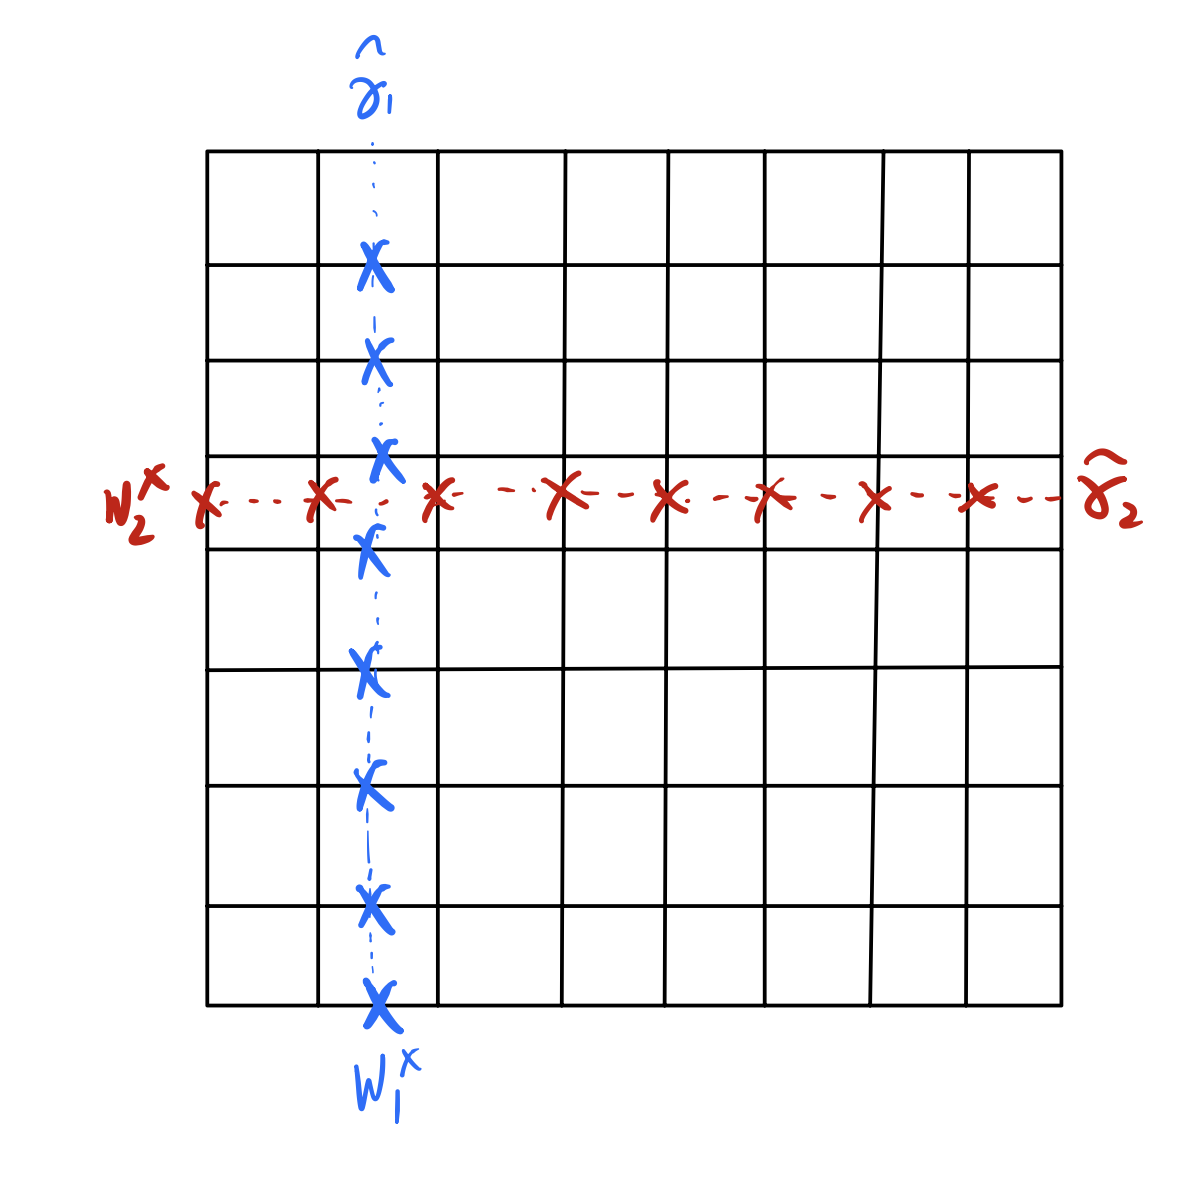
\includegraphics[scale=0.3]{Lectures/Images/lec3-strings.png}
\end{center}

Thus we end up the matrix elements:
\begin{equation}
    \bra{\Omega, \pm, \pm}W\ket{\Omega, \pm, \pm} \sim \lambda^L\text{diag}(c_1, c_2, c_3, c_4)
\end{equation}
and so then the splitting between the ground states is:
\begin{equation}
    \delta \sim \lambda^L = e^{-L\log(\frac{1}{\lambda})}
\end{equation}
Note that this is quite heuristic, and to make it rigorous you require more precise arguments, namely that the perturbation theory converges, with a finite radius of convergence $\lambda_0$ (which holds for arbitrarily large $L$). Without a formal argument, we expect such a finite radius of convergence for ``typical'' gapped local Hamiltonians, with $\lambda_0 \sim \Delta$ (so actually, in addition to the local indistinguishability, we are also using that the toric code is gapped).

\subsection{A Review of Berry Phase}
Before we move to a general discussion of anyons, we first review the notion of a Berry phase, which is a very related idea.

Let:
\begin{equation}
    \set{\ket{\psi(s)}, 0 \leq s \leq T, \ket{\psi(T)} = e^{i\phi}\ket{\psi(0)}}
\end{equation}
be a closed path in the set of normalized quantum states (rays in Hilbert space). Let us split up the path into $N$ parts of length $\Delta s$, with $N\Delta s = T$. Graphically:

\begin{center}
    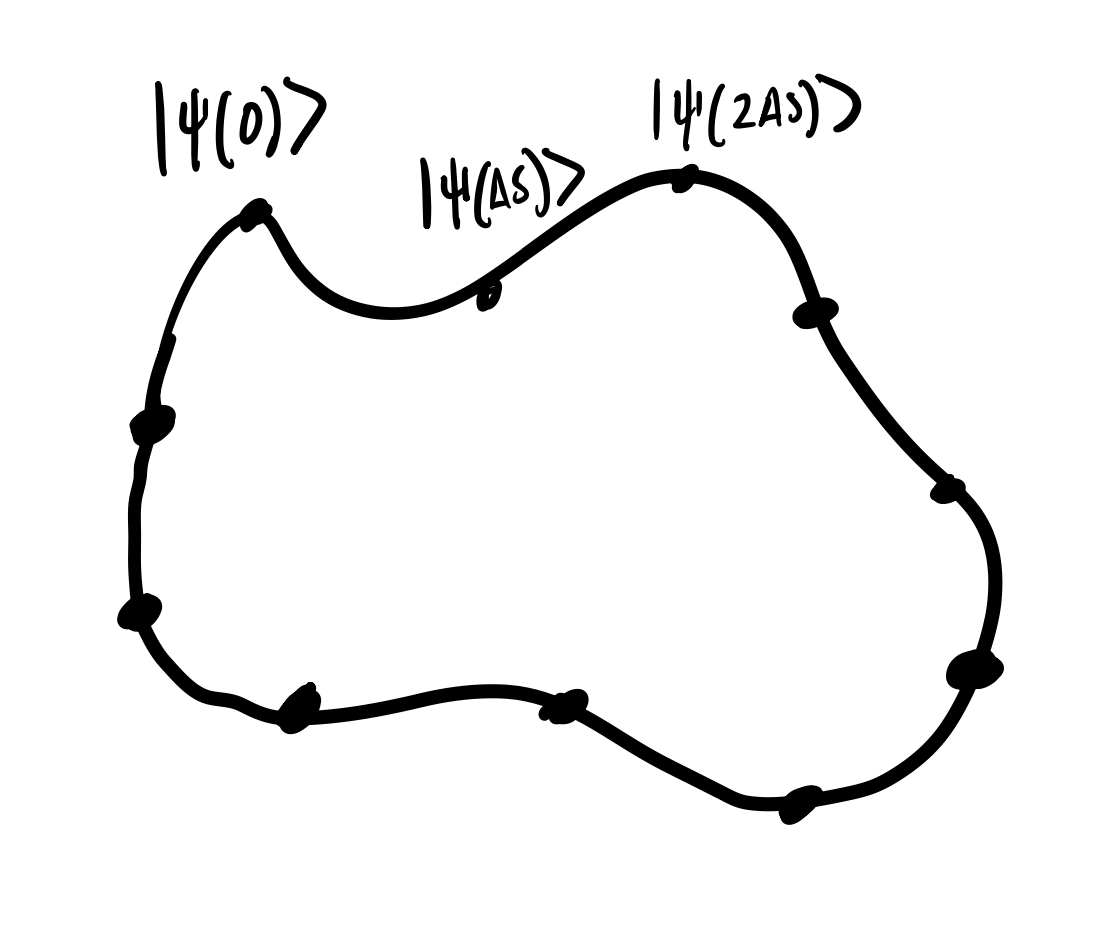
\includegraphics[scale=0.3]{Lectures/Images/lec3-berryphasepath.png}
\end{center}

and for brevity we denote $\ket{\psi(\cdot)} = \ket{\psi_\cdot}$. Now, we define the Berry phase as:
\begin{equation}
    e^{i\theta_B} = \lim_{N \to \infty}\braket{\psi_0}{\psi_{N-1}}\ldots\braket{\psi_2}{\psi_1}\braket{\psi_1}{\psi_0}
\end{equation}
The Berry phase has properties:
\begin{enumerate}
    \item $\abs{e^{i\theta_B}} = 1$, i.e. $e^{i\theta_B}$ is a $U(1)$ phase. This can be seen from the fact that $\braket{\psi_1}{\psi_0} \sim \frac{1}{N}$ and so the $N$-fold product is of order $\sim 1$.
    \item $e^{i\theta_B}$ only depends on the path and not its parameterization. That is, it is invariant under $s \to s' = f(s)$ with $f(0) = 0$ and $f(T) = T'$.
    \item $e^{i\theta_B}$ does not depend on the phase of $\ket{\psi(s)}$. That is, it is invariant under $\ket{\psi(s)} \to e^{i\varphi(s)}\ket{\psi(s)}$. This is easily seen from the definition - the phase of the ket is cancelled out by that of the bra in the $N$-fold product.
\end{enumerate}
Taking the limit $N \to \infty$, we have the formula:
\begin{equation}
    \theta_B = \int_0^T ds\phantom{i} i\bra{\psi(s)}\dod{}{s}\ket{\psi(s)}
\end{equation}
there is however the caveat when we evaluate the Berry phase in this way. We have to add the assumption that $\ket{\psi(0)} = \ket{\psi(T)}$ without the phase factor.

\subsection{Berry phase and adiabatic evolution}
The Berry phase shows up in two places; in adiabatic processes/cycles, and in path integrals. Today, we talk about the former.

First, a reminder of the adiabatic theorem. Let $H(t)$ be a time-dependent Hamiltonian with $0 \leq t \leq T$. Suppose $H(t)$ has a unique ground state $\ket{\psi(t)}$ with energy $E(t)$ and gap $\Delta(t)$. Suppose $H(t)$ varies on a timescale $\tau \gg \frac{1}{\min_t \Delta (t)}$. Then:
\begin{equation}
    \ket{\psi(0)} \stackrel{\text{evolve under } H(t)}{\longrightarrow} (\text{phase})\ket{\psi(t)}.
\end{equation}

Now, consider a closed path $H(T) = H(0)$, which we may consider an ``adiabatic cycle''. 

\begin{center}
    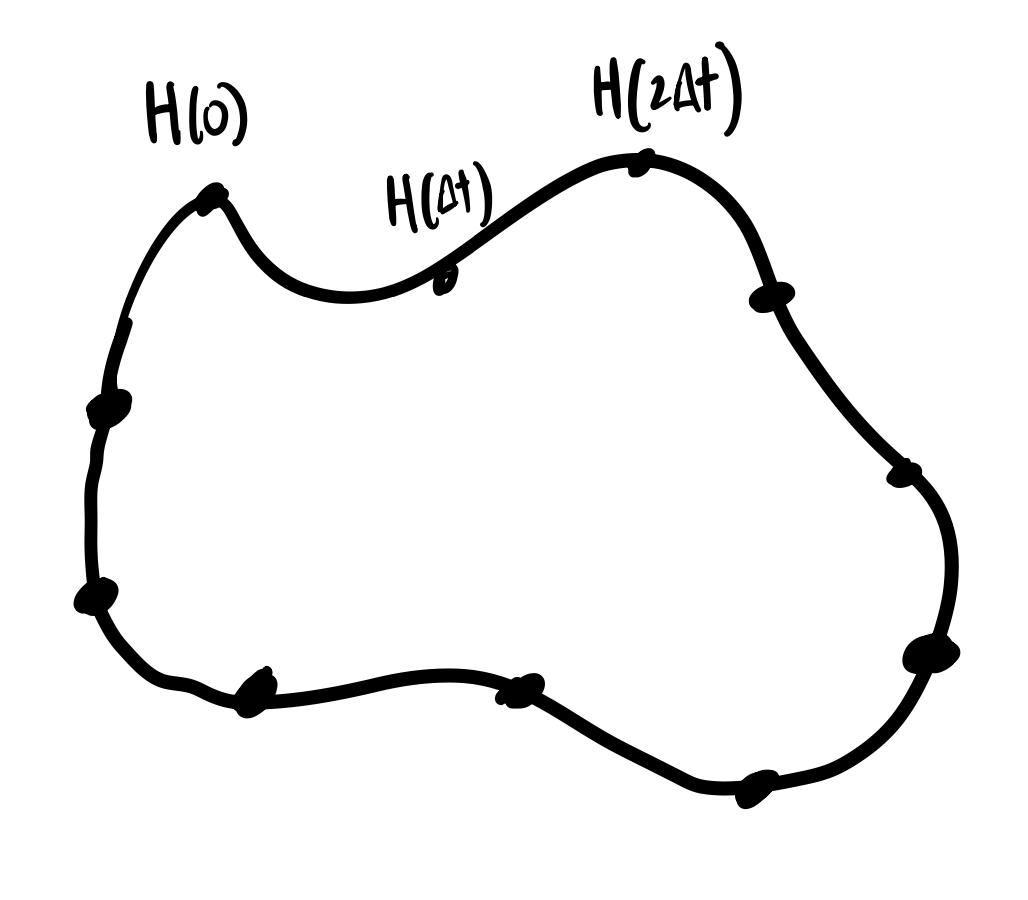
\includegraphics[scale=0.3]{Lectures/Images/lec3-Hpath.png}
\end{center}

Then:
\begin{equation}
    \ket{\psi(0)} \stackrel{\text{evolve}}{\longrightarrow} (\text{phase})\ket{\psi(0)}
\end{equation}
Let's compute this phase factor! It is given by:
\begin{equation}
    (\text{phase}) = \bra{\psi(0)}\mathcal{T}\exp(-i\int_0^T dt H(t))\ket{\psi(0)}
\end{equation}
with $\mathcal{T}$ denoting time ordering. We compute the phase factor by discritizing the time-dependent Hamiltonian to $H(0) = H_0, H(\Delta t) = H_1, H(2\Delta t) = H_2, \ldots$ with $N\Delta t = T$ and associated instantaneous ground states $\ket{\psi(0)} = \ket{\psi_0}, \ket{\psi(\Delta t)} = \psi_1, \ldots$. Then the expression for the phase factor becomes:
\begin{equation}
    (\text{phase}) = \lim_{N \to \infty }\bra{\psi(0)}e^{-i\Delta tH_{N-1}}e^{-i\Delta tH_{N-2}}\ldots e^{-i\Delta tH_{1}}e^{-i\Delta tH_{0}}\ket{\psi(0)}
\end{equation}
According to the adiabatic theorem, we know that:
\begin{equation}
    e^{-i\Delta t H_0}\ket{\psi_0} = \dyad{\psi_1}{\psi_1}e^{-i\Delta t H_0}\ket{\psi_0}
\end{equation}
as the adiabatic evolution takes $\ket{\psi_0} \to \ket{\psi_1}$ in the first time interval. We can thus insert projectors about each time step:
\begin{equation}
    (\text{phase}) = \lim_{N \to \infty }\bra{\psi(0)}e^{-i\Delta tH_{N-1}}\dyad{\psi_{N-1}}{\psi_{N-1}}e^{-i\Delta tH_{N-2}}\dyad{\psi_{N-2}}{\psi_{N-2}}\ldots \dyad{\psi_{2}}{\psi_{2}}e^{-i\Delta tH_{1}}\dyad{\psi_{1}}{\psi_{1}}e^{-i\Delta tH_{0}}\ket{\psi(0)}
\end{equation}
Each of the expectation values only gives a phase factor of the energy, and so:
\begin{equation}
    (\text{phase}) =  \lim_{N \to \infty }\exp(-i\Delta t \sum_{k=0}^{N-1}E_k)\braket{\psi_0}{\psi_{N-1}}\ldots\braket{\psi_2}{\psi_1}\braket{\psi_1}{\psi_0}
\end{equation}
and so:
\begin{equation}
    \boxed{(\text{phase}) = \exp(-i\int_0^T E(t)dt)e^{i\theta_B}}
\end{equation}
i.e. we have a path-dependent dynamical phase part and a Berry phase part.

We'll stop here for now, and next time we will discuss the Berry phase associated with anyons.
\section{Abelian Anyons I}

Today we discuss anyons and derive them from first principles. We focus on the 2-D case in our discussion.

\subsection{Single-particle Berry Phase}
Let $H$ be a 2-D gapped Hamiltonian with short-ranged interactions (sum of local terms). Suppose $H$ has a particle-like excitation (the rough idea is that there is a state in $\mathcal{H}$ that looks like the ground state everywhere, except for a localized region in space). In general, these excitations/particles can be in different locations in space\footnote{Physically, we could imagine these $\v{r}$ as minima of some trapping potential} $\v{r}$. For each different position, we will have a distinct many-body state, which we can label as $\ket{\v{r}}$. We can then consider the Berry phase $\theta_B(\gamma)$ associated with a closed path $\gamma$:
\begin{equation}
    \theta_B(\gamma) = \int_0^T \bra{\v{r}(t)}i\dod{}{t}\ket{\v{r}(t)}dt
\end{equation}

\begin{center}
    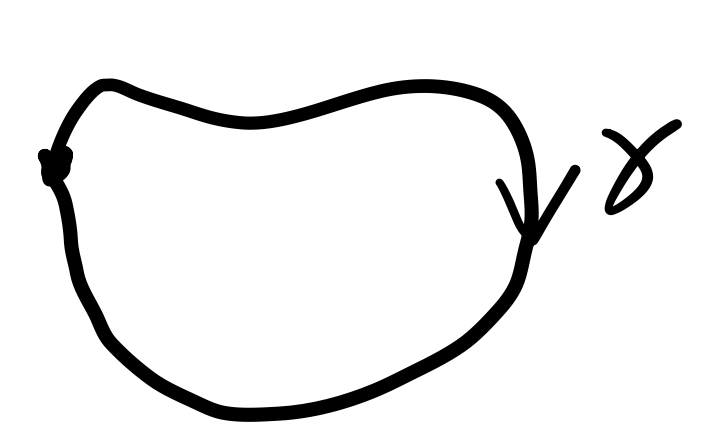
\includegraphics[scale=0.3]{Lectures/Images/lec4-path.png}
\end{center}

We can define the Berry connection, which is a vector:
\begin{equation}
    \gv{\mathcal{A}}(\v{r}) = \bra{\v{r}}i\nabla_\v{r}\ket{\v{r}} = \m{\bra{\v{r}}i\dpd{}{x}\ket{\v{r}} \\ \bra{\v{r}}i\dpd{}{y}\ket{\v{r}}}
\end{equation}
Using the chain rule, we are able to write the berry phase as an integral over the Berry connection:
\begin{equation}
    \theta_B(\gamma) = \int_\gamma\gv{\mathcal{A}}(\v{r})\cdot d\v{r}
\end{equation}
a comment; this looks a lot like a vector potential (and indeed this choice of notation is not a coincidence); the effect that $\gv{\mathcal{A}}$ has on the physics is the same as if the particle was coupled to a background vector potential/magnetic field $\v{A}$. This has very little to do with anyons - but when we go to multiple particles, we see the physics of anyons start to emerge.

\subsection{Multi-particle Berry Phase and the Locality constraint}
The extra part that appears when we look at the multi-particle Berry phase is exchange statistics (and this is how we will ``see'' anyons emerge)! Consider a state with $n$ identical excitations/particles, which we can parameterize by $\ket{\set{\v{r}_1, \ldots \v{r}_n}}$. Since the particles are identical, we need not specify the order, only the positions.

Now, let us consider the Berry phase associated with an $n$-particle closed path $\Gamma$. A picture of this path directly is a bit tricky (e.g. for 2 particles we have a 4-dimensional configuration space, which is not even Euclidean due to the lack of ordering). But we can draw it as particle worldlines through time, e.g. for four particles:

\begin{center}
    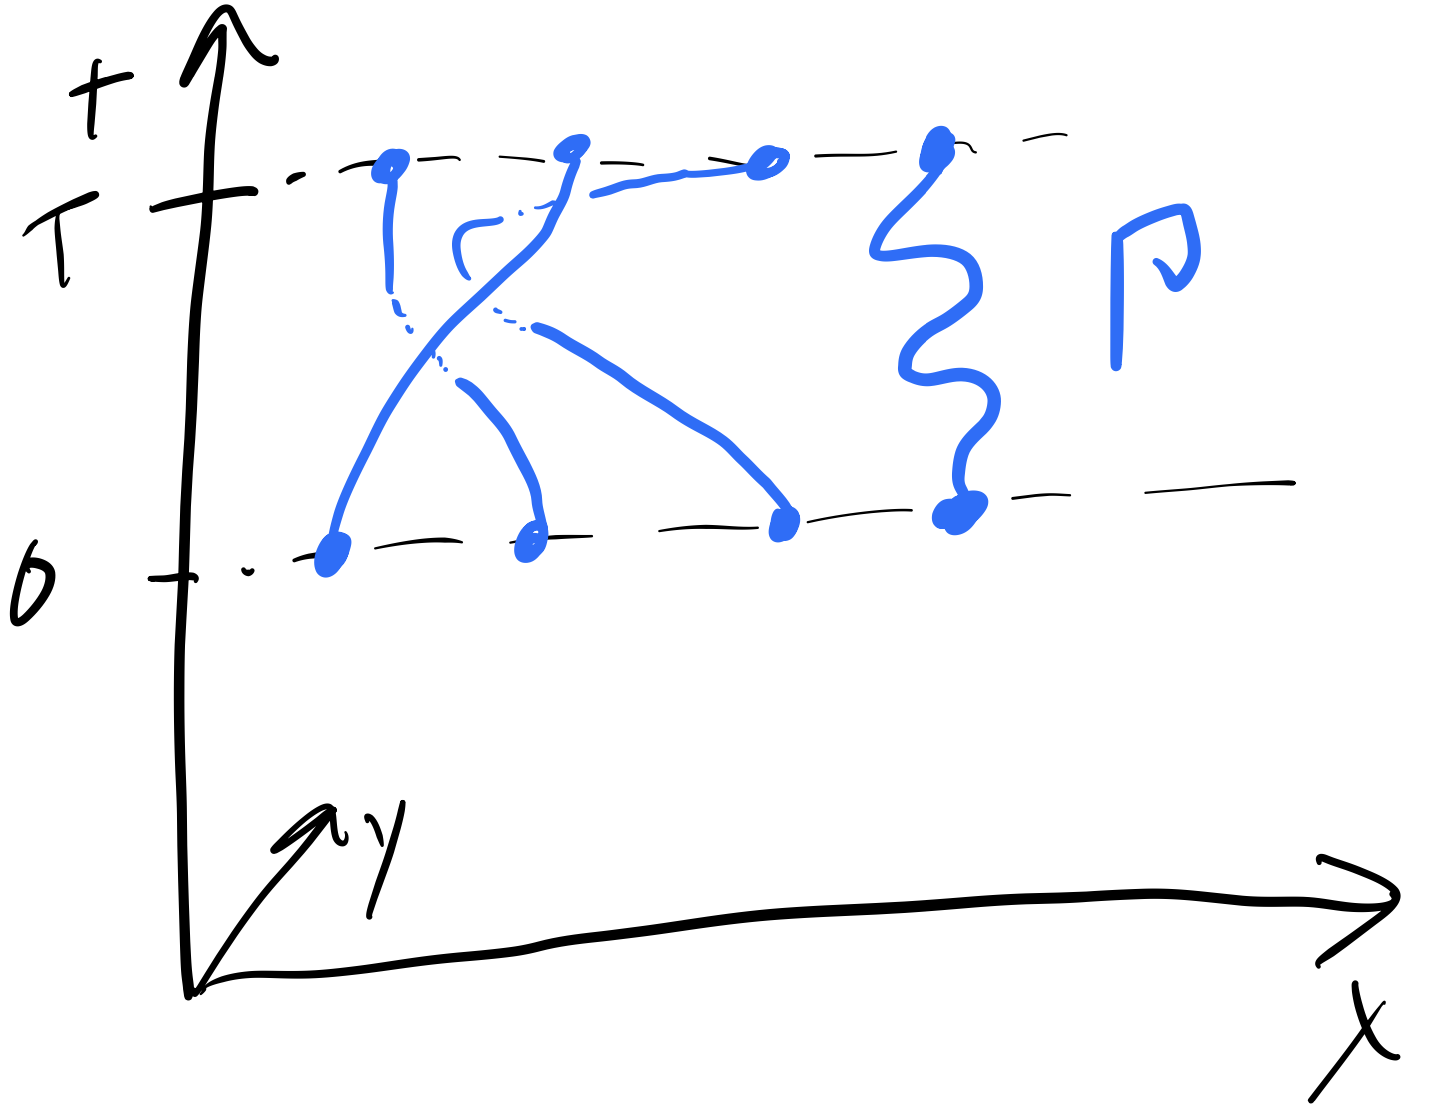
\includegraphics[scale=0.3]{Lectures/Images/lec4-worldlines.png}
\end{center}

The Berry phase is then:
\begin{equation}
    \theta_B(\Gamma) = \int_0^T \bra{\set{\v{r}_1(t), \ldots \v{r}_n(t)}}i\dod{}{t} \ket{\set{\v{r}_1(t), \ldots \v{r}_n(t)}} dt
\end{equation}
The question to understand is then; what does this look like? What are general constraints on $\theta_B$? The answer is that $\theta_B$ has to be ``local''. More precisely, imagine modifying a multi-particle path $\Gamma$ near $(\v{r}_0, t_0)$:

\begin{center}
    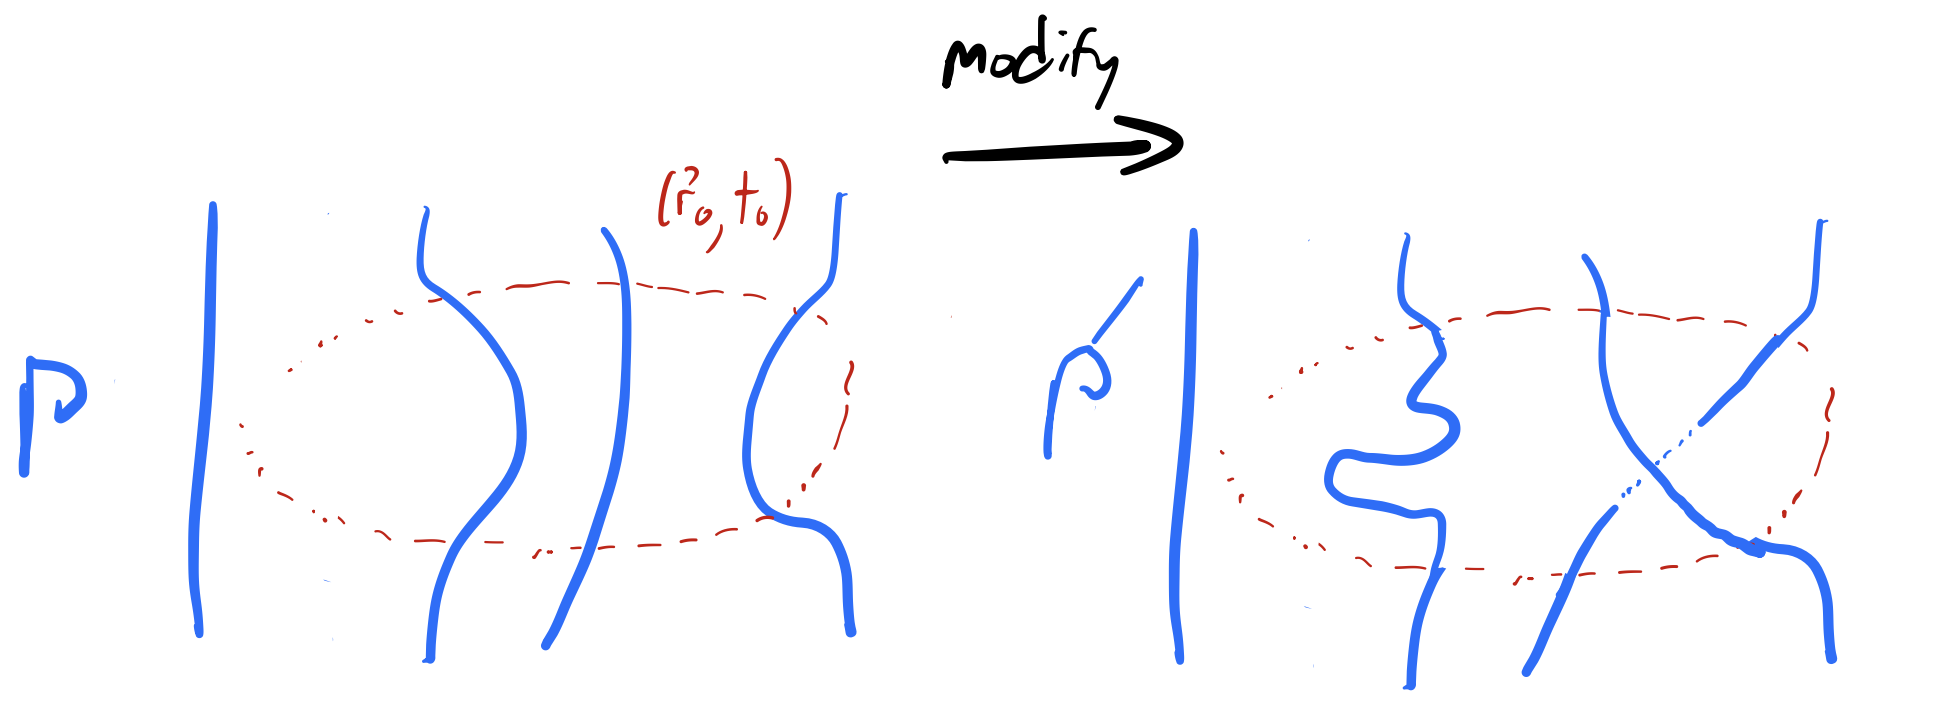
\includegraphics[scale=0.3]{Lectures/Images/lec4-localgammamod.png}
\end{center}

Then, $\theta_B(\Gamma') - \theta_B(\Gamma)$ depends only on what $\Gamma, \Gamma'$ look like near $(\v{r}_0, t_0)$. In other words:
\begin{equation}\label{eq:berryphasediff}
    \theta_B(\Gamma') - \theta_B(\Gamma) = \theta_B(\Lambda') - \theta_B(\Lambda)
\end{equation}
if $\Lambda, \Lambda'$ looks like $\Gamma, \Gamma'$ near $(\v{r}_0, t_0)$ and differ by the same local move:

\begin{center}
    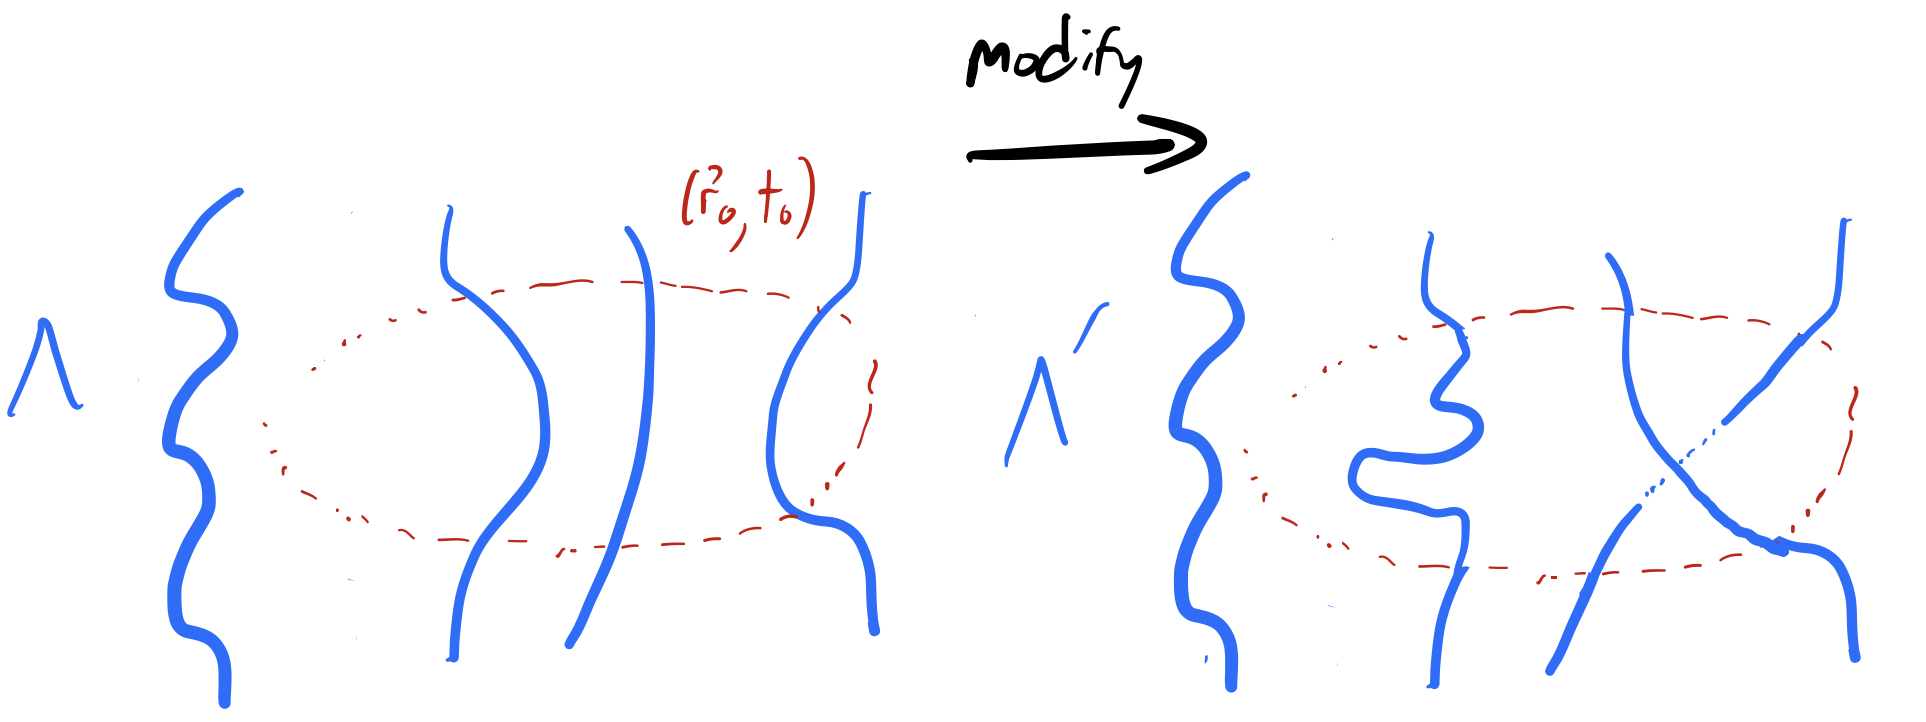
\includegraphics[scale=0.3]{Lectures/Images/lec4-localdeltamod.png}
\end{center}

The claim is local change near $(\v{r}_0, t_0)$ is insensitive to faraway modifications. Why does Eq. \eqref{eq:berryphasediff} hold? It is because the difference in Berry phase $\theta_B(\Gamma') - \theta_B(\Gamma)$ can be measured by a local operator acting near $(\v{r}_0, t_0)$ (Physically, we can imagine an interference or adiabatic experiment there). The equation then follows, assuming:
\begin{enumerate}
    \item $\ket{\Psi} = \ket{\set{\v{r}_1, \ldots \v{r}_n}}$ has short-ranged correlations, i.e.:
    \begin{equation}
        \avg{A_\v{r}A_{\v{r}'}'}_\Psi = \avg{A_\v{r}}_\Psi\avg{A_{\v{r}'};}_\Psi + \mathcal{O}(e^{-\frac{\abs{\v{r} - \v{r}'}}{\xi}})
    \end{equation}
    for $A_\v{r}, A_{\v{r}'}$ local operators supported near $\v{r}, \v{r}'$. This is where the gapped assumption comes in; the ground state of a gapped Hamiltonian has short-ranged correlations.
    \item Particles can be moved by local operators. In other words:
    \begin{equation}
        \ket{\set{\v{r}_1', \v{r}_2, \ldots, \v{r}_n}} = M\ket{\set{\v{r}_1, \ldots, \v{r}_n}}
    \end{equation}
    where $M$ is an operator supported near $\v{r}_1, \v{r}_1'$.
    \begin{center}
        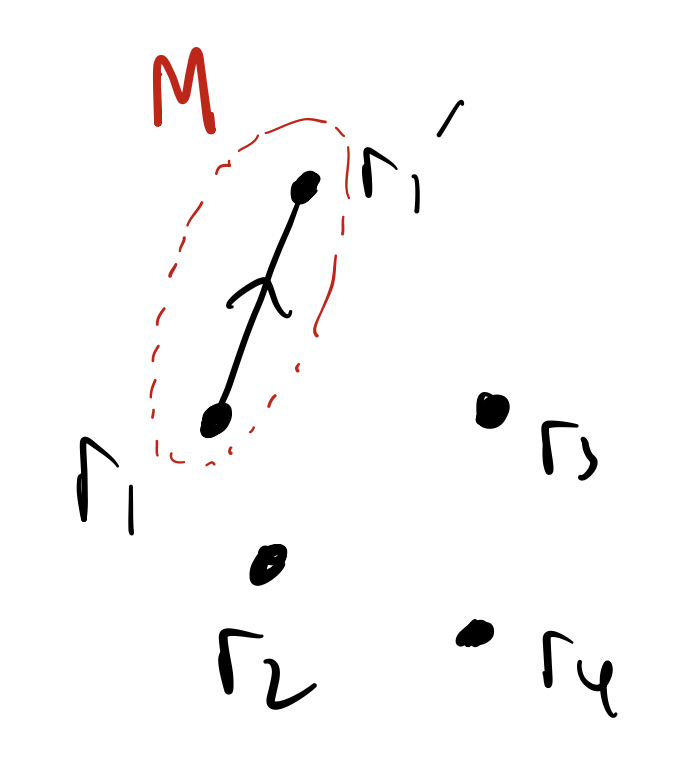
\includegraphics[scale=0.3]{Lectures/Images/lec4-Mlocal.png}
    \end{center}
\end{enumerate}
These two conditions together imply the locality constraint on the Berry phase.

\subsection{Possible Forms of the Berry Phase \& Topological Classes}
The next question is then - what is the most general Berry phase $\theta_B(\Gamma)$ that satisfies the locality constraint? One solution, and the one you probably would have guessed, is:
\begin{equation}
    \theta_B(\Gamma) = \sum_i\int_\Gamma\gv{\mathcal{A}}(\v{r}_i)\cdot d\v{r}_i.
\end{equation}
This is manifestly local. We could get a little more general:
\begin{equation}\label{eq:thetabshortrange}
    \theta_B(\Gamma) = \sum_i\int_\Gamma\left(\gv{\mathcal{A}}(\v{r}_i) + \sum_j \gv{\mathcal{B}}(\v{r}_i, \v{r}_j) + \sum_{jk}\gv{\mathcal{C}}(\v{r}_i, \v{r}_j, \v{r}_k) + \ldots\right)\cdot d\v{r}_i
\end{equation}
where $\gv{\mathcal{A}}$ is the single-particle Berry connection and $\gv{\mathcal{B}}, \gv{\mathcal{C}}$ are the two, three (and so on) particle terms so long as the multi-particle terms are short-ranged, i.e. only they are nonzero where $\v{r}_j$ is close to $\v{r}_i$ and so on. 

Is this the only possible solution consistent with Eq. \eqref{eq:berryphasediff}? No! Indeed the first proposed solution is the form of the Berry phase consistent with bosons, but there are other solutions corresponding to fermions and anyons. What does the first solution miss? Indeed it is possible to have topological terms that look highly non-local, but such that the Berry phase still has the locality constraint.

In this line, we say that two (non-intersecting) $n$-particle paths with the same endpoints are topologically equivalent if they can be continuously deformed into one another without bringing particles near each other (worldlines cannot pass through one another). For example, consider:

\begin{center}
    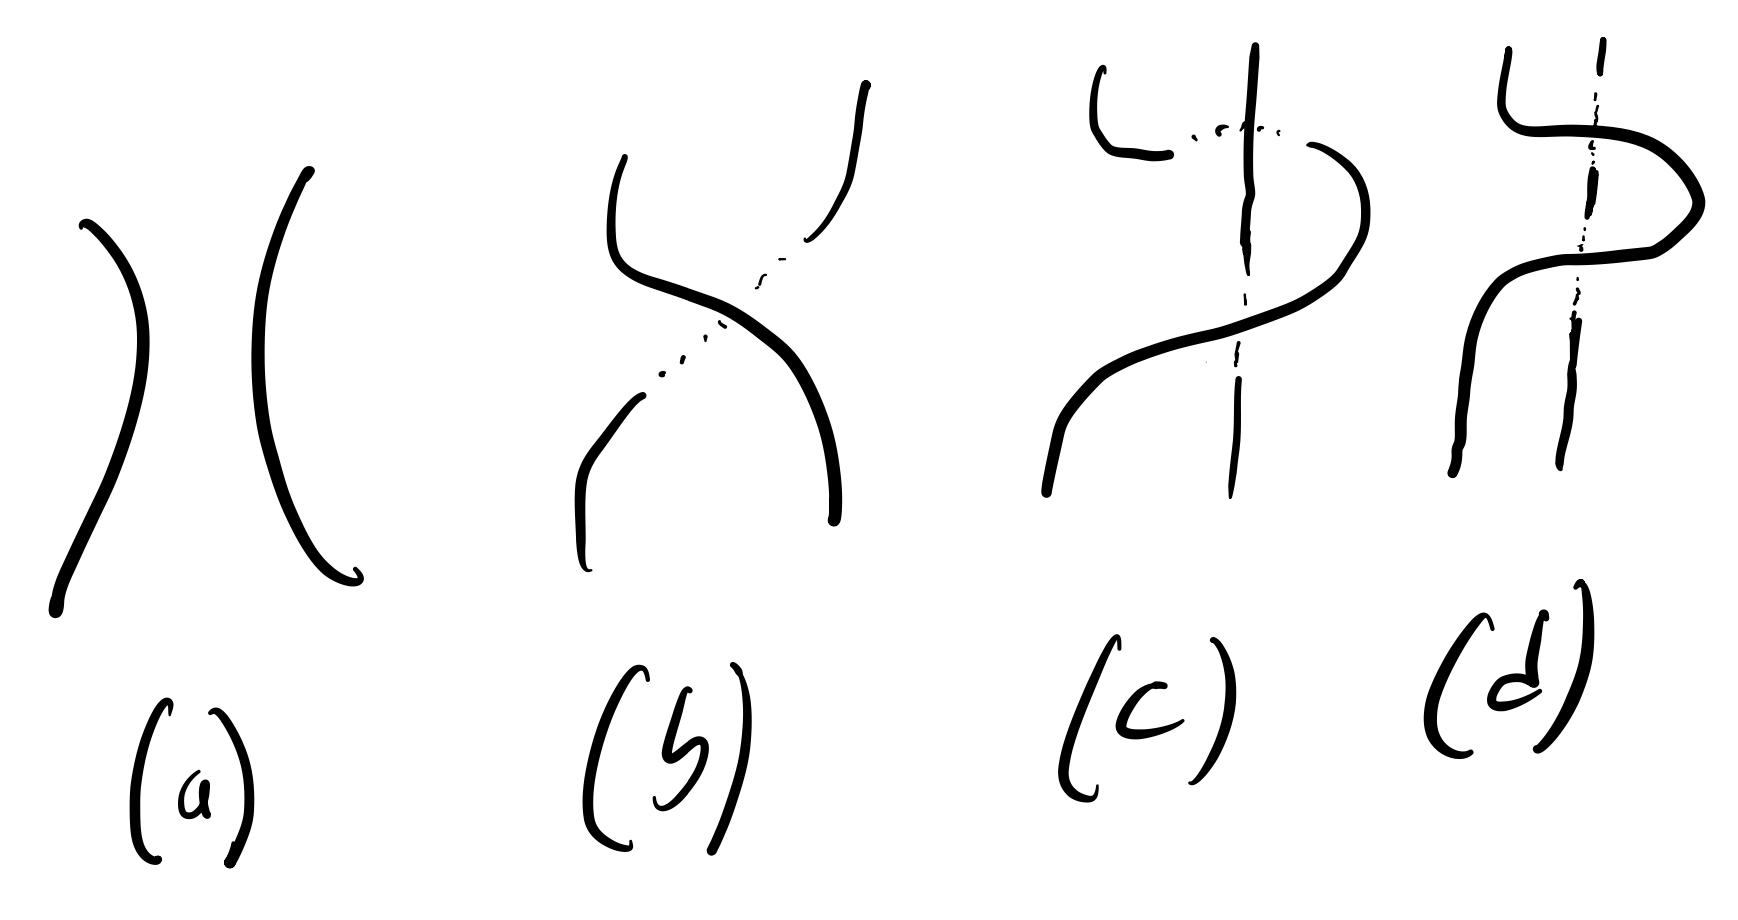
\includegraphics[scale=0.3]{Lectures/Images/lec4-topclasses.png}
\end{center}

$(a) \sim (d)$, but $(a) \not\sim (b) \not\sim (c)$. This defines an equivalence relation on (non-intersecting) $n$-particle paths, which splits the set of $n$-particle paths into equivalence (topological) classes. 

Coming back to the Berry phase, the claim is that the most general $\theta_B$ that satisfies the locality constraint Eq. \eqref{eq:berryphasediff} can be written as:
\begin{equation}\label{eq:berryphasetypes}
    \boxed{\theta_B(\Gamma) = \theta_{\text{short-range}}(\Gamma) + \theta_{\text{top}}(\Gamma)}
\end{equation}
where $\theta_{\text{top}}(\Gamma)$ only depends on the topological class of $\Gamma$ and the short-range piece is given by Eq. \eqref{eq:thetabshortrange}
\begin{equation}
    \theta_{\text{short-range}}(\Gamma) = \sum_i\int_\Gamma\left(\gv{\mathcal{A}}(\v{r}_i) + \sum_j \gv{\mathcal{B}}(\v{r}_i, \v{r}_j) + \sum_{jk}\gv{\mathcal{C}}(\v{r}_i, \v{r}_j, \v{r}_k) + \ldots\right)\cdot d\v{r}_i.
\end{equation}
Eq. \eqref{eq:berryphasetypes} is the key result. From here, we will classify the different possible topological terms we can have. We will find in 3D that we only get two possible classes and in 2D that we get many more.

Let us argue for Eq. \eqref{eq:berryphasetypes} in the special case of $\Gamma$ being a topologically trivial path, i.e. where we only have the first term. For the sake of drawing, let's look at a 2 particle path.
\begin{equation}
    \theta_B(\Gamma) = \theta_B(\gamma_1 \& \gamma_2) = ?
\end{equation}
\begin{center}
    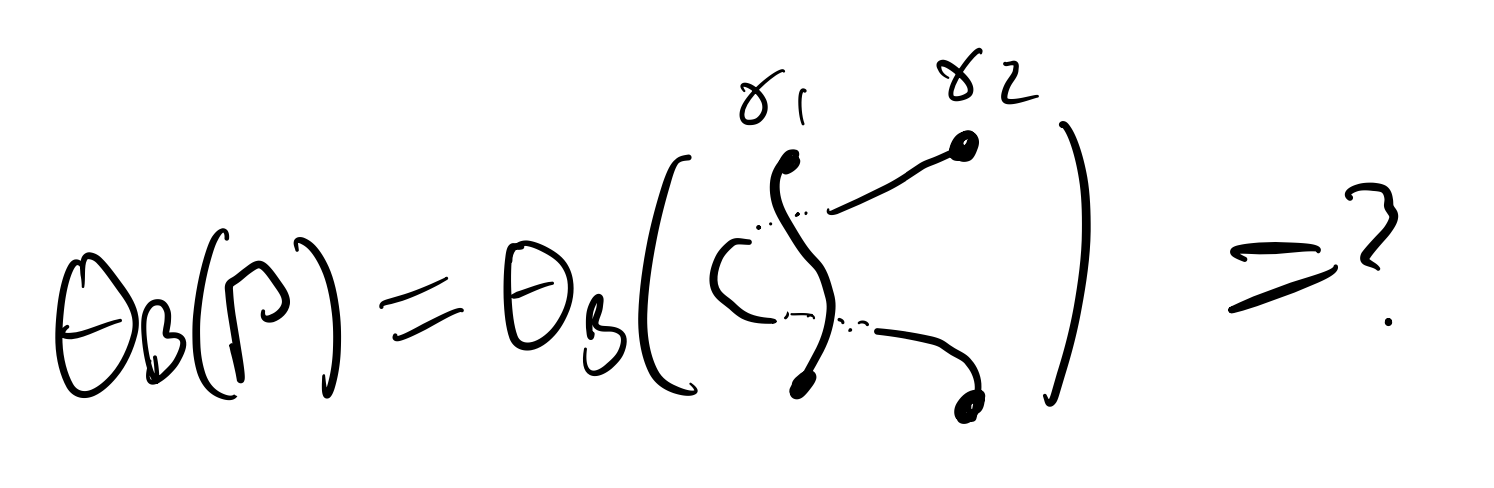
\includegraphics[scale=0.3]{Lectures/Images/lec4-thetaBtwo.png}
\end{center}
where $\gamma_1, \gamma_2$ are the single particle paths. We can then define:
\begin{equation}
    \Delta(\Gamma) = \theta_B(\gamma_1 \& \gamma_2) - \theta_B(\gamma_1) - \theta_B(\gamma_2)
\end{equation}
Now, using Eq. \eqref{eq:berryphasediff} we can use that $\Delta(\Gamma)$ is topologically invariant, i.e. it is invariant to local deformations of $\gamma_1$ far from $\gamma_2$ and vise versa. 

\begin{center}
    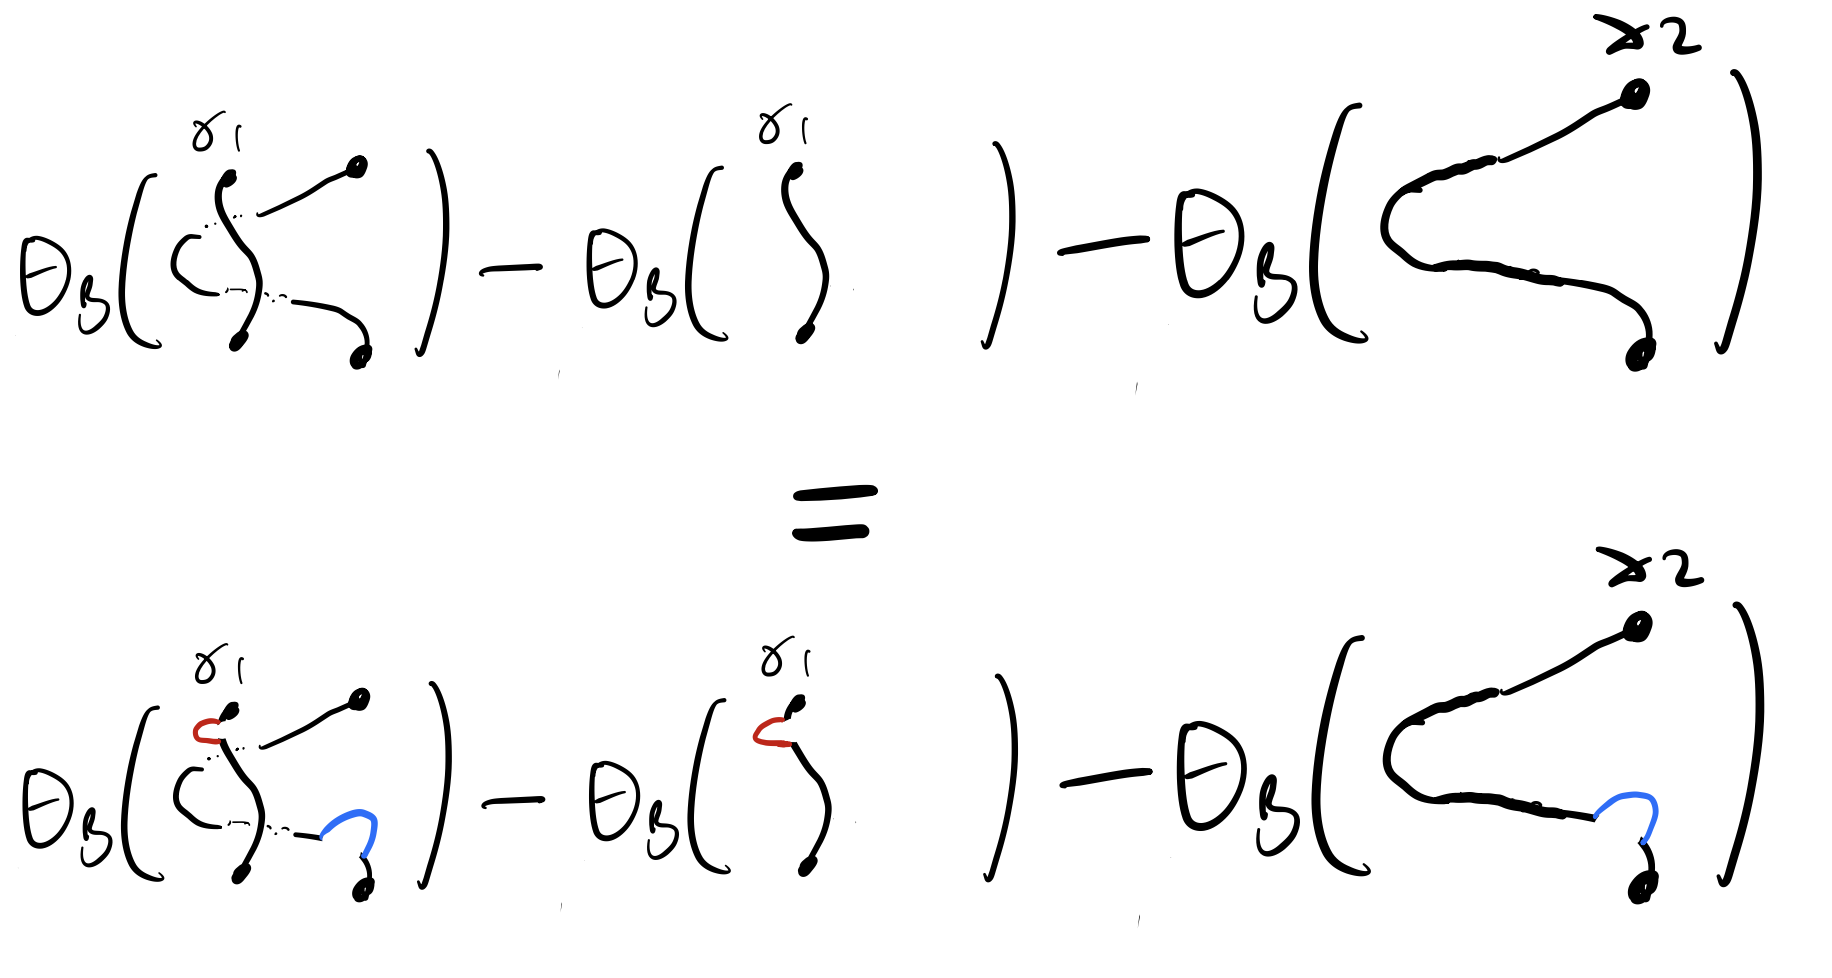
\includegraphics[scale=0.3]{Lectures/Images/lec4-thetaBequiv.png}
\end{center}

Therefore we can deform $\Gamma$ to the trivial path, for which $\Delta$ is easily seen to vanish.
\begin{equation}
    \Delta(\Gamma) = \Delta(\Gamma_{\text{trivial}}) = 0
\end{equation}

\begin{center}
    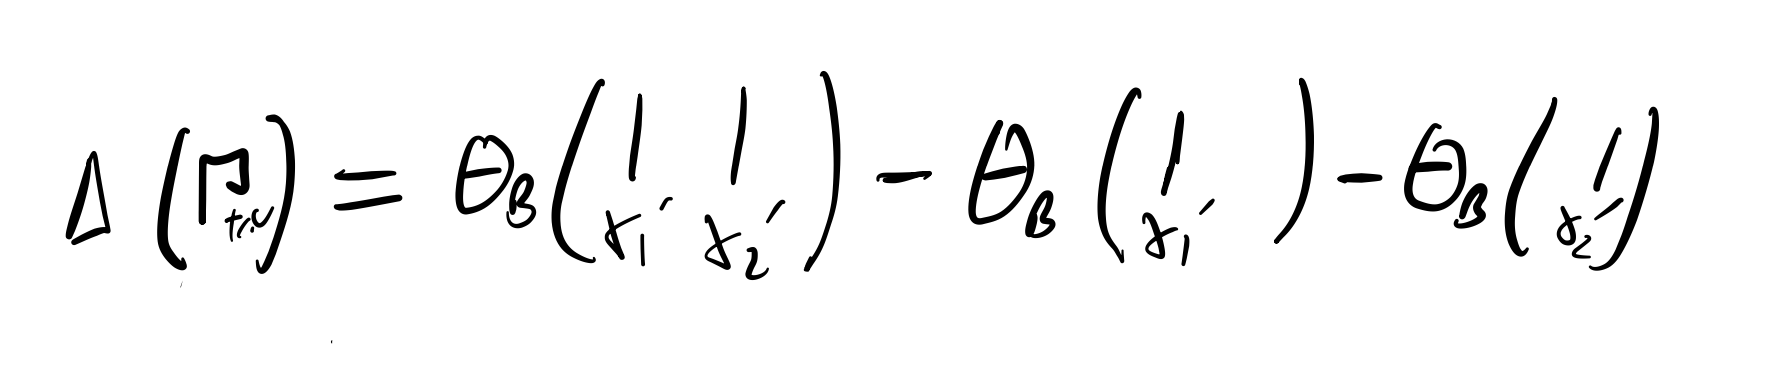
\includegraphics[scale=0.3]{Lectures/Images/lec4-thetaBtriv.png}
\end{center}

And thus since $\Delta(\Gamma) = 0$, we find:
\begin{equation}
    \theta_B(\Gamma) = \theta_B(\gamma_1) + \theta_B(\gamma_2) = \int_{\gamma_1}\v{\mathcal{A}}(\v{r}_1) \cdot d\v{r}_1 + \int_{\gamma_2}\v{\mathcal{A}}(\v{r}_2) \cdot d\v{r}_2 = \theta_{\text{short-range}}(\Gamma).
\end{equation}

\section{Quantum double model and non-Abelian anyons I}
\section{Abelian Anyons III, Quantum Double Model I}

\subsection{Mutual Statistics of Toric Code Anyons}
We want to compute the mutual statistics of charge and flux statistics $e^{i\theta_{\text{em}}}$ in the Toric code. The strategy was to compare two paths, $\Gamma$ and $\Gamma'$ (see figure from last lecture) such that the paths look the same, but $\Gamma$ has a flux in the center of the path and $\Gamma'$ has a flux outside of it. By looking at the difference of the two processes, since the two paths ``look the same'', the uninteresting short-range contributions to the phase will cancel, leaving us with just $\theta_{\text{em}}$:
\begin{equation}
    \theta(\Gamma) - \theta(\Gamma') = \theta_{\text{em}}
\end{equation}
where $\theta(\Gamma), \theta(\Gamma')$ are the total phases accumulated by some sequence of local movement operators. Let's compute these and now see what we get. The simplest operator we can write down to move charges is $Z_j$ - the pauli-$Z$ operator on link $j$. This moves a charge from site $s$ to site $s'$ (and vise versa), as depicted in the figure from last lecture (the figure is slightly poorly notated; it should really depict movement of charges, as opposed to swapping the site labels. The precise action is captured in the anticommutation, or in the relations of Eq. \eqref{eq:applyZ}). We can see this from the anticommutation of $Z_j$ with $A_s, A_{s'}$.

Denote the initial state by $\ket{p_0, s}$. Let $\Gamma$ denote the process composed out of a sequence of $Z$ operators, which moves the charge $s$ along the path $\gamma$.

\begin{center}
    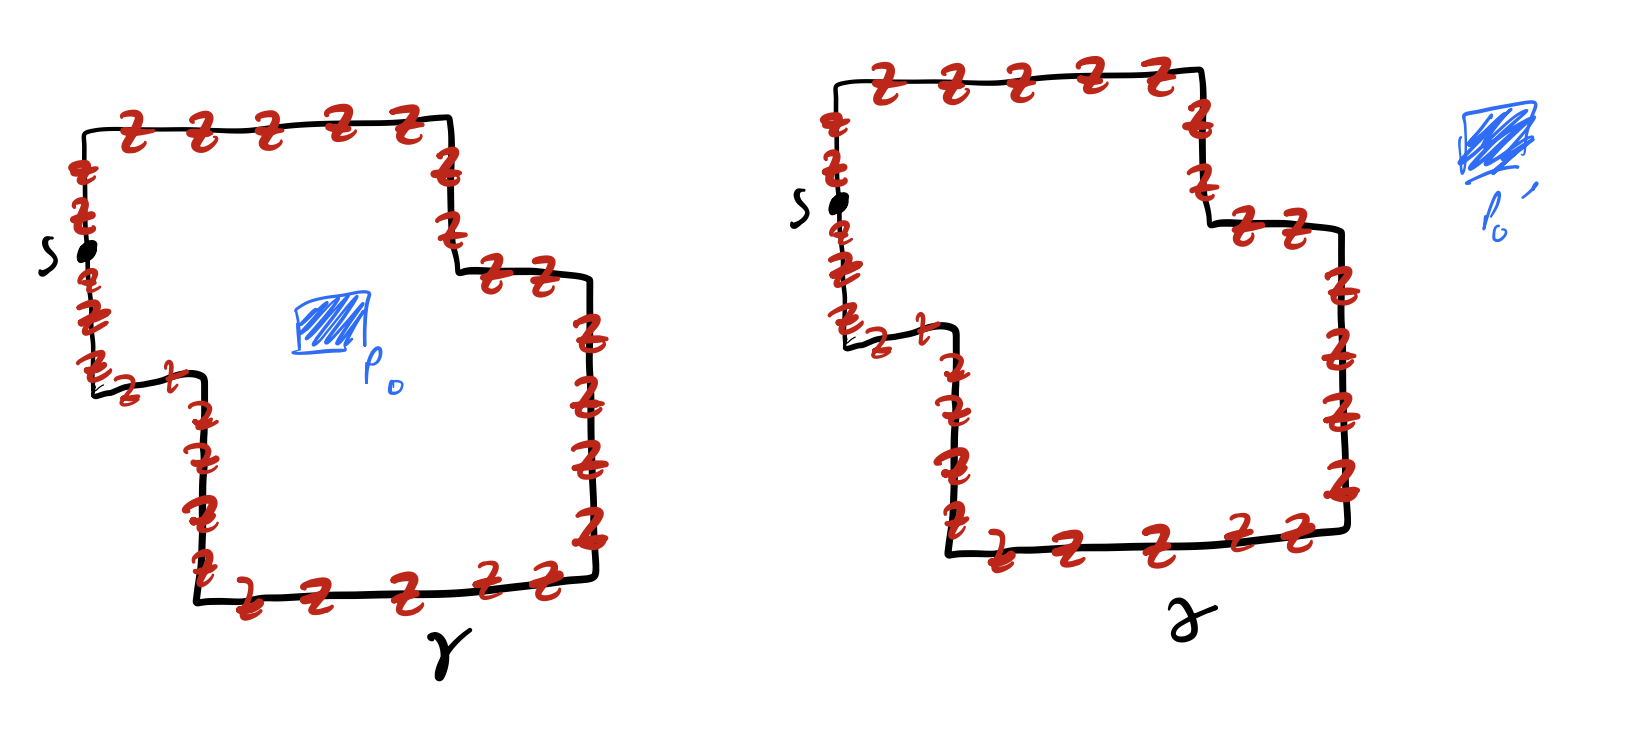
\includegraphics[scale=0.35]{Lectures/Images/lec6-twopaths.png}
\end{center}

By definition:
\begin{equation}
    \prod_{j \in \gamma}Z_j \ket{p_0, s} = e^{i\theta(\Gamma)}\ket{p_0, s}
\end{equation}
To figure out what $e^{i\theta(\Gamma)}$, we observe the operator identity:
\begin{equation}
    \prod_{j \in \gamma}Z_j = \prod_{p \in \text{int}(\gamma)}B_p
\end{equation}
Note that this is a kind of Stokes' theorem. We can use this identity to evalute $e^{i\theta(\Gamma)}$ - we're in business because there is exactly one $b_p = -1$ inside of $\gamma$:
\begin{equation}
    e^{i\theta(\Gamma)}\ket{p_0, s} = \prod_{p \in \text{int}(\gamma)}B_p\ket{p_0, s} = -\ket{p_0, s}
\end{equation}
Thus:
\begin{equation}
    e^{i\theta(\Gamma)} = -1
\end{equation}
We aren't quite done yet. We should compare this to the case where the flux is not in the center. Now, consider $\Gamma'$ which is an identical process save for the flux is on a plaquette $p_0'$ outside of the path $\gamma$. Then:
\begin{equation}
    e^{i\theta(\Gamma')}\ket{p_0', s} = \prod_{j \in \gamma}Z_j \ket{p_0', s} = \prod_{p \in \text{int}(\gamma)}B_p\ket{p_0', s} = +\ket{p_0', s}
\end{equation}
where the last equality follows since all $b_p = +1$ in the interior of the path (the only flux is outside). Thus:
\begin{equation}
    e^{i\theta(\Gamma')} = 1
\end{equation}
Therefore looking at the difference:
\begin{equation}
    e^{i\theta_m} = e^{i\theta(\Gamma)}e^{-i\theta(\Gamma')} = -1 \cdot 1 = -1
\end{equation}
Thus:
\begin{equation}
    \boxed{e^{i\theta_m} = -1}
\end{equation}
We compared two phases, one which was nontrivial and one which was trivial, and then the ratio gives us the interesting exchange statistic. 

Why was it important that we took the difference between these two paths/compared the two processes? We chose $Z$ as our movement operator, but someone else could have very well chosen $e^{i\phi}Z$ for any phase; then that random phase would contribute to $e^{i\theta(\Gamma)}$ and $e^{i\theta(\Gamma')}$. But crucially, it contributes in the exact same way to both of these, and hence does not contribute to the difference.

A couple remarks:
\begin{enumerate}
    \item The result does not depend on the microscopic details of the path $\gamma$. We expected this from what we know about the Berry phase, but also saw this clearly arise from the calculation itself. Moreover, $\theta_{\text{em}}$ does not depend on the choice of movement operator; we won't prove this in full generality, but we did remark how movement operators differing by a phase give the same result. In fact even if the movement operators look more starkly different, we find the same result.
    \item Mutual statistics are symmetric, and indeed we could swap the roles of the charges/fluxes and $Z/X$ and we would get the same results.
    \item According to the definition from last class, $e, m$ are indeed non-trivial anyons since $e^{i\theta_{\text{em}}} = -1$ (non-trivial mutual statistics, with each other).
    \item We could also ask what the mutual statistics of taking an $e$ particle around itself (or $m$ around itself). Then, its trivial to show that:
    \begin{equation}
        e^{i\theta_{\text{ee}}} = e^{i\theta_{\text{mm}}} = 1
    \end{equation}
    \item Note that an even number of charges/fluxes look like having no charges/fluxes at all. Actually, we have four types of ``sectors'' of excitations $\set{1, e, m, \e}$ with $1$ being even charges/fluxes, $e$ being odd charges even fluxes, $m$ being even charges odd fluxes, and $\e$ being odd charges and fluxes (you will study this one on the homework).
\end{enumerate}

\subsection{Connection between Abelian Anyons and String Operators}
We sketch the connection between mutual statistics and the algebra of string operators. In the previous section we gave a physically transparent way of computing mutual statistics, now we give the shortcut. Let $a, b$ be Abelian anyons, and let $W_a, W_b$ be associated string operators. $W_a$ creates an excitation $a$ at one end and its antiparticle $\bar{a}$ at its other end (in the toric code, the particles and antiparticles coincide). Consider paths $\gamma, \beta$, and then compare:
\begin{equation}
    W_a(\gamma)W_b(\beta)\ket{\Omega}, \quad  W_b(\beta)W_a(\gamma)\ket{\Omega}
\end{equation}

\begin{center}
    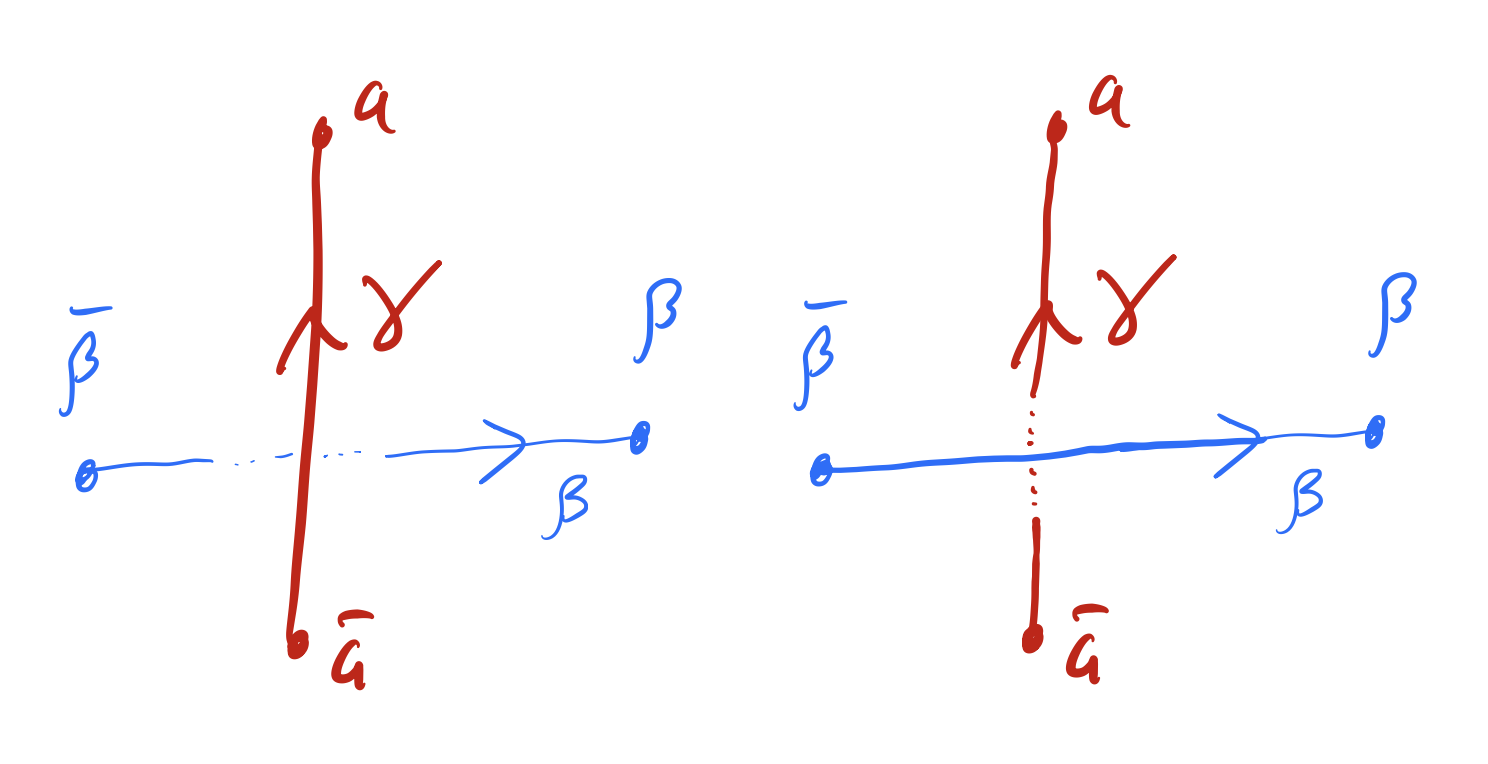
\includegraphics[scale=0.35]{Lectures/Images/lec6-stringoporder.png}
\end{center}

The claim is then:
\begin{equation}\label{eq:stringopmutualstat}
    W_a(\gamma)W_b(\beta)\ket{\Omega} = e^{i\theta_{ab}} W_b(\beta)W_a(\gamma)\ket{\Omega}
\end{equation}

For example, lets use $a = e, b = m$ on the toric code. The $b$-string is a string of $X$s that creates two fluxes on the end, and the $a$-string in a string of $Z$s that creates two charges on the end:

\begin{center}
    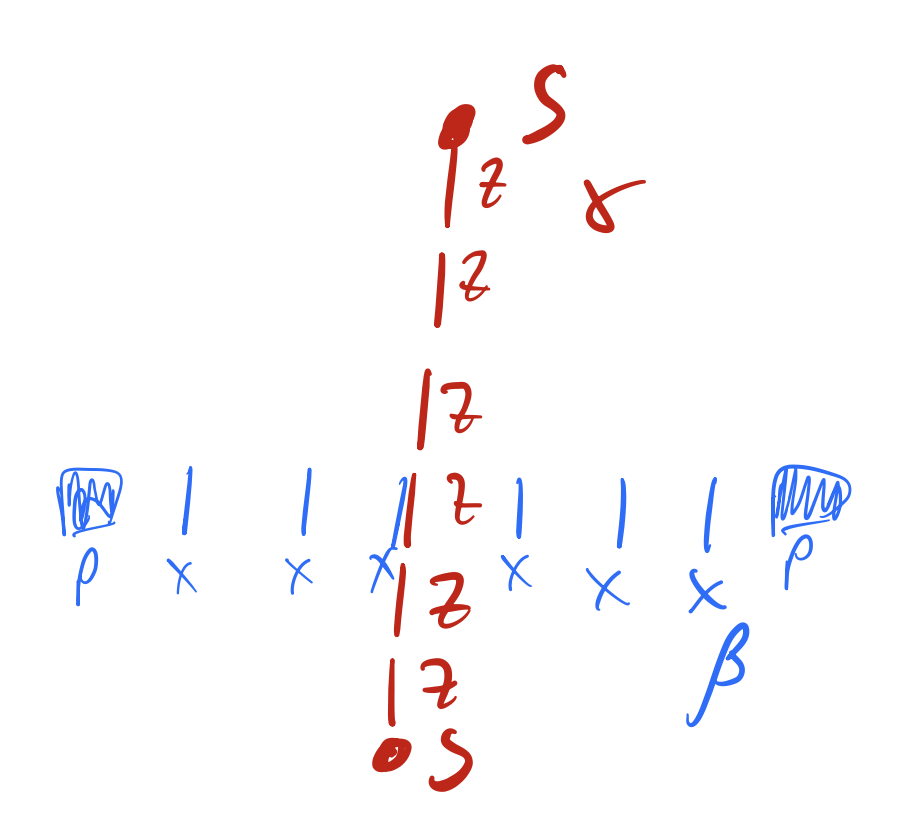
\includegraphics[scale=0.35]{Lectures/Images/lec6-stringopanticommute.png}
\end{center}

These two operators anticommute on the operator level:
\begin{equation}
    W_e(\gamma)W_m(\beta) = -W_m(\beta)W_e(\gamma)
\end{equation}
and hence also anticommute when acted upon the ground state. Thus:
\begin{equation}
    e^{i\theta_{\text{em}}} = -1
\end{equation}

Let us derive the general relation of Eq. \eqref{eq:stringopmutualstat}. On general grounds, we know that:
\begin{equation}
    W_a(\gamma)W_b(\beta)\ket{\Omega} = e^{i\theta}W_b(\beta)W_a(\gamma)\ket{\Omega}
\end{equation}
for \emph{some} phase $\theta$. This is because both of the states correspond to the creation of anyons on both sides - hence both states have the same 4 anyons ($a, \bar{a}, b, \bar{b}$) at the same locations. Hence they must describe the same physical state. To compute the phase, we multiply both the right and left hand side with a further string operator, $W_a(\gamma')$:
\begin{equation}
    W_a(\gamma')W_a(\gamma)W_b(\beta)\ket{\Omega} = e^{i\theta} W_a(\gamma')W_b(\beta)W_a(\gamma)\ket{\Omega}
\end{equation}

Graphically, the LHS/RHS look like:

\begin{center}
    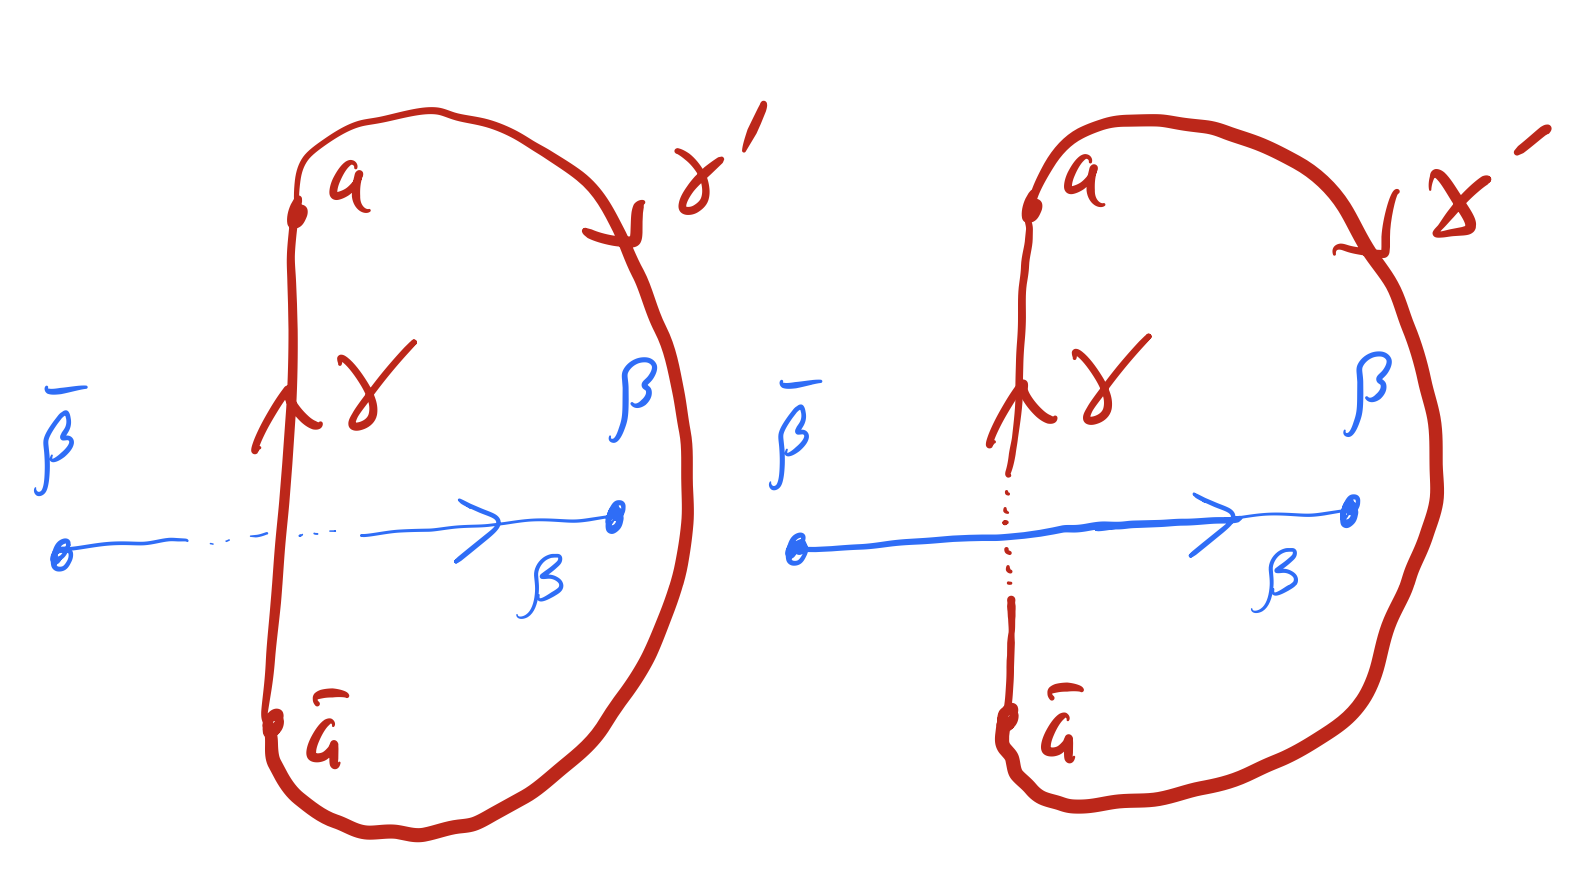
\includegraphics[scale=0.35]{Lectures/Images/lec6-braid.png}
\end{center}

The first thing we see at an algebraic level is that $W_a(\gamma')$ commutes with $W_b(\beta)$, as they act on non-overlapping places:
\begin{equation}
    W_a(\gamma')W_a(\gamma)W_b(\beta)\ket{\Omega} = e^{i\theta} W_b(\beta)W_a(\gamma')W_a(\gamma)\ket{\Omega}
\end{equation}
Now let's think about the two processes we have here. On the LHS, we have that $a$ braids around $b$ (we first create $b$ and then do the big loop). On the RHS, we first create $a, \bar{a}$ and do the big loop, and then create $b$ - $a$ follows the exact same path, but does $\emph{not}$ braid around $b$. Thus, we would conclude that the phase difference $\theta$ must be the topological Berry phase $\theta_{ab}$, as everything else cancels.

To summarize:
\begin{enumerate}[(a)]
    \item Abelian anyon excitations $\iff$ non-commuting flexible string operators (with the algebra of the SOs encoding the mutual statistics. On the HW, you will also see that the algebra of the SOs imply exchange statistics, but this will require looking at three string operators)
    \item Non commuting flexible string operators $\implies$ Robust GSD (on torus)
    \item Robust GSD $\implies$ robust quantum memory (can encode the qubit in the GSD).
\end{enumerate}
Thus any system with Abelian anyons has all these properties... it is harder to formulate the reverse statement, but easy counterexamples don't come to mind.

\subsection{Introduction to the Quantum Double Model}
The above concludes our discussion of abelian anyons and the toric code. We thus move onto the discussion of non-abelian anyons and the quantum double model. The reference is \texttt{quant-ph/9707021}. 

We can think of the quantum double model as the generalization of the toric code. It's not actually a single model, but a class of models, of which we specify a specific model by choice of a finite group $G$. The toric code corresponds to choosing $G = \ZZ_2$ (the simplest nontrivial choice). Looking a bit ahead, when we choose $G$ to be Abelian, the model will host Abelian anyons, but when we choose $G$ to be a non-Abelian group, the quantum double model will host non-Abelian anyon excitations.

What are non-Abelian anyons? In short, Abelian if we trap $n$ particles at $n$ sites have a unique physical state, vs. for non-Abelian anyons the same process results in a ground state with degeneracy. We will see that the braiding processes for these anyons will not be Abelian.

We have a local Hilbert space on each edge site of a lattice, with each edge Hilbert space having dimension $\abs{G}$. 

\begin{center}
    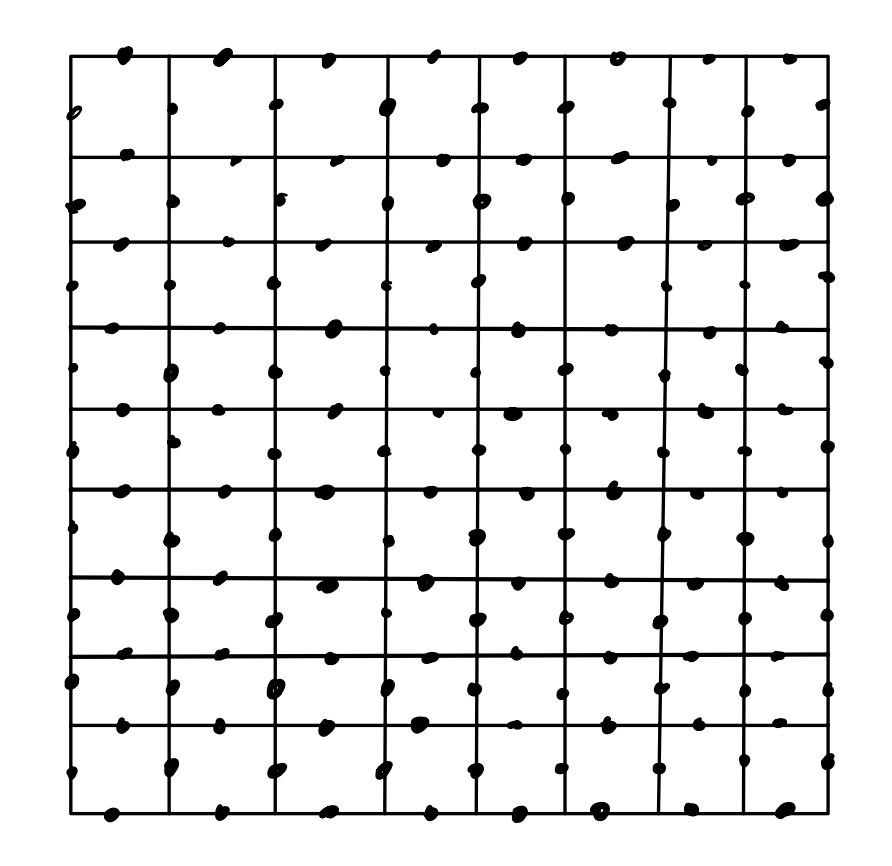
\includegraphics[scale=0.35]{Lectures/Images/lec6-lattice.png}
\end{center}

It is convenient to define two orthonormal basis for each edge, $\set{\uparrow\ket{g}}$ and $\set{\downarrow\ket{g}}$ where $g \in G$. The $\uparrow/\downarrow$ correspond to the orientation of the link. The relationship between these two bases are very simple:
\begin{equation}
    \uparrow\ket{g} = \downarrow\ket{g^{-1}}
\end{equation}
For example:

\begin{center}
    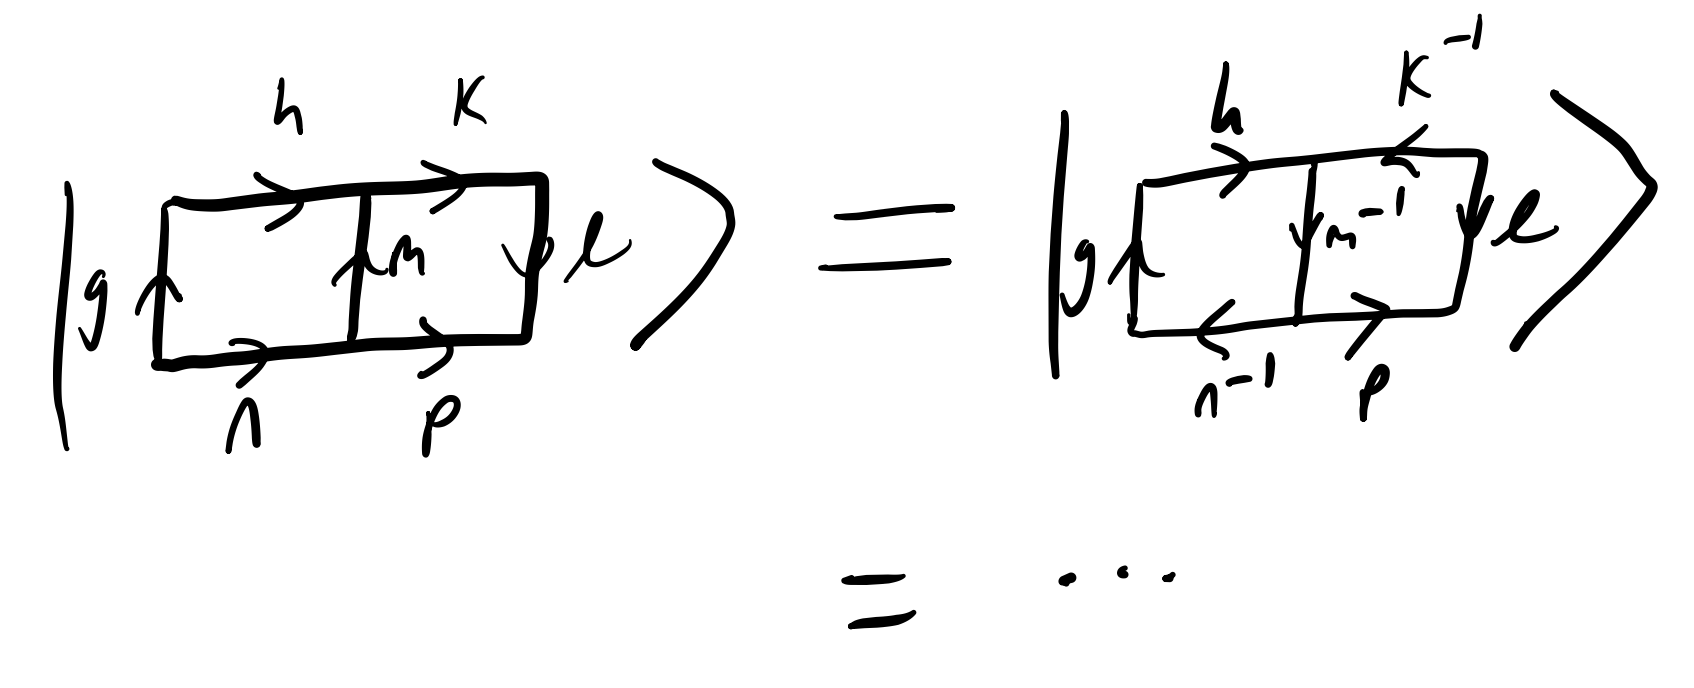
\includegraphics[scale=0.35]{Lectures/Images/lec6-inverse.png}
\end{center}

We're out of time for today, but it's worth noting that quantum double model with group $G$ is related to $G$-gauge theory; just written in a more concrete way. In such a gauge theory, to transport a charge in the gauge theory along a link you use unitary $g/g^{-1}$ depending on which direction you want to transport it.

\section{Quantum Double Model II}
Like the toric code, we consider a lattice of local Hilbert spaces; except unlike the toric code where each on-site hilbert space was $\CC^2$ (a qubit), now the model is defined by a group $G$ with the Hilbert space at each site having dimension $\abs{G}$. There is a set of two orthnormal bases for each edge, $\set{\uparrow\ket{g}}, \set{\downarrow\ket{g}}$ where $g \in G$, with the property that flipping the direction of the arrow flips $g \to g^{-1}$. This is captured in the last figure we drew last time.

We might ask why we might not fix an orientation convention. We could do this, but it does break some symmetries in the model. So it's better to keep a ``free global'' orientation. 

\subsection{Hamiltonian for the Quantum Double Model}
We introduce two types of operators $A_g(s), B(p)$. These are related, but do not exactly coincide with the operators in the toric code.

We start with the star operator $A_g(s)$, which graphically has the action:

\begin{center}
    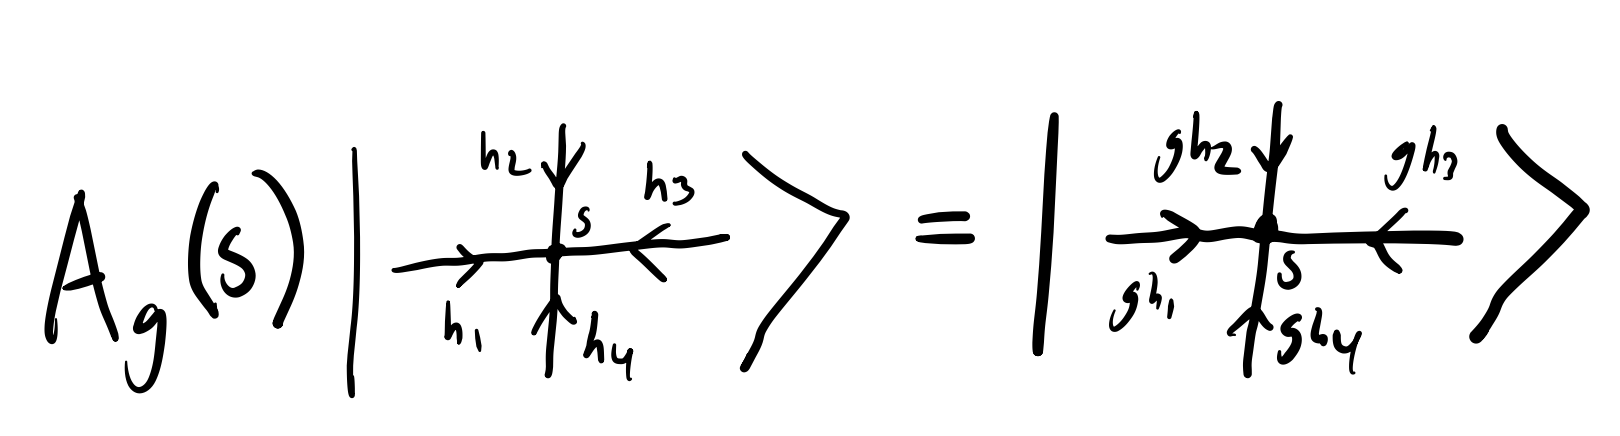
\includegraphics[scale=0.35]{Lectures/Images/lec7-Agaction.png}
\end{center}

in other words it permutes between bases elements via left-multiplication of $g$ on edges that are part of the star. It is sometimes called a ``gauge transformation''. Note that incoming arrows get left-multiplied by $g$ and outgoing arrows get right-multiplied by $g^{-1}$ (but we will derive this explicitly, we only need specify the action on incoming arrows).

The plaquette operator has the action:

\begin{center}
    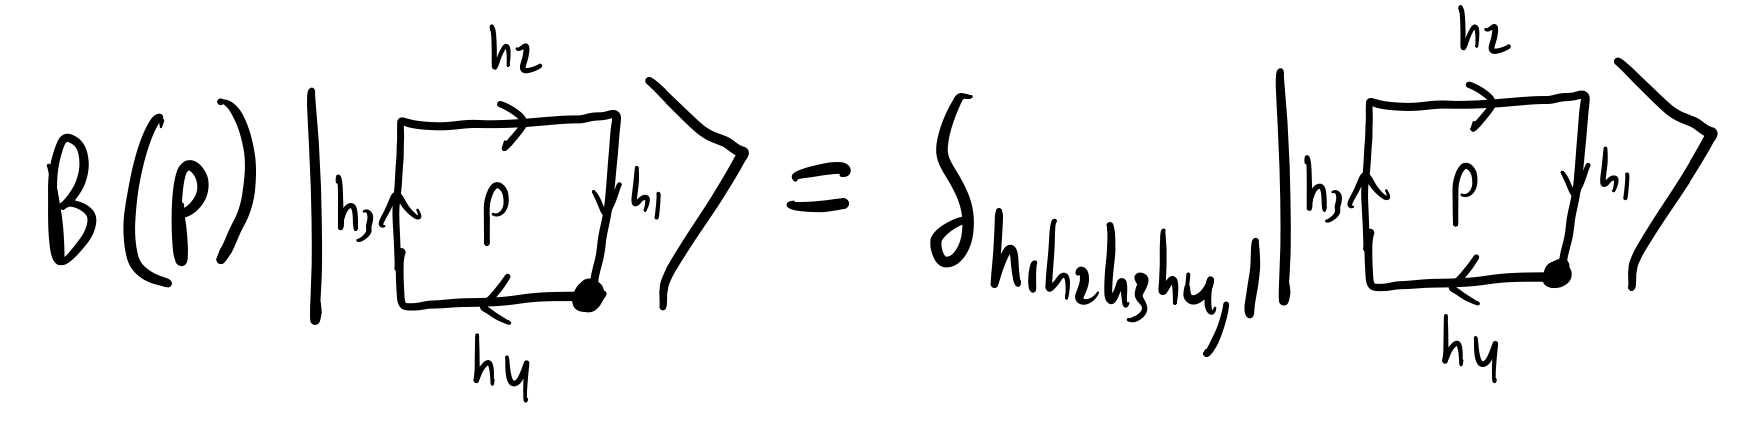
\includegraphics[scale=0.35]{Lectures/Images/lec7-Baction.png}
\end{center}

where:
\begin{equation}
    \delta_{h_1h_2h_3h_4, 1} = \begin{cases}
        1 & h_1h_2h_3h_4 = 1
        \\ 0 & \text{otherwise}
    \end{cases}
\end{equation}
The terminology we will use is that $h_1h_2h_3h_4$ is the ``flux through the plaquette $p$''.

There is a bit of convention with the multiplication of the group elements, in that we start with the basepoint in the bottom right and go around counterclockwise. We might ask that does this basepoint choice matter? If we started in the top right, we would instead get:
\begin{equation}
    h_2h_3h_4h_1 = h_1^{-1}(h_1h_2h_3h_4)h_1
\end{equation}
so concretely, different base points change flux by conjugation. But since the identity element is unchanged by conjugation, and here we only care about fluxes as identity, it will turn out to not matter here (in fact we could go in the other direction, and this changes the sign of the flux, but because the identity is self-inverse it again does not matter here. But it will matter when we look at some related operators).

Another comment; $B(p)$ are diagonal in the group element basis, while $A_g(s)$ are not. 

Now, defining the Hamiltonian in terms of these operators:
\begin{equation}
    H = - \sum_s A(s) - \sum_p B(p)
\end{equation}
where:
\begin{equation}
    A(s) = \frac{1}{\abs{G}}\sum_g A_g(s)
\end{equation}

A couple comments about this Hamiltonian. Let's check to make sure that it is indeed Hermitian. $B(p)$ is clearly Hermitian, because in our chosen orthonormal basis it is real and diagonal in the group element basis. To see that $A(s)$ is Hermitian requires a tiny bit of work. First, we notice that $A_g(s)$ is a unitary operator (because it is a permutation matrix):
\begin{equation}
    A_g(s)^\dag = A_g(s)^{-1}
\end{equation}
But since $A_g(s)$ acts via left multiplication of $g$, $A_g(s)^{-1}$ should be a left multiplication by $g^{-1}$:
\begin{equation}
    A_g(s)^\dag = A_{g}(s)^{-1} = A_{g^{-1}}(s).
\end{equation}
This tells us that in general $A_g(s)$ will not be Hermitian. But the sum will be! This is because:
\begin{equation}
    A(s)^\dag = \left(\frac{1}{\abs{G}}\sum_g A_g(s)\right)^\dag = \frac{1}{\abs{G}}\sum_{g}A_{g^{-1}}(s) = \frac{1}{\abs{G}}\sum_g A_g(s) = A(s)
\end{equation}
as the sum over all inverses of group elements is the same as the sum over all group elements.

So, the $H$ is Hermitian, and hence a valid Hamiltonian.

\subsection{Relationship to the Toric Code}
Suppose we set $G = \ZZ_2 = \set{1, g}$ with $g^2 = 1$. Then on each link we have two states; we can identify $\ket{1} \leftrightarrow \ket{Z = 1}$ and $\ket{g} \leftrightarrow \ket{Z = -1}$ with $Z$ the standard Pauli operator. We can then see what the star and plaquette operators reduce to:
\begin{equation}
    A(s) = \frac{1}{2}(A_1(s) + A_g(s)) = \frac{\II + \prod_{j \in \text{star}(s)}X_s}{2}= \frac{\II + A_s}{2}
\end{equation}
So we get the projector onto the star operator of the toric code. The same holds for $B(p)$; to have a product of group elements equal to 1 in $\ZZ_2$, this means we need an even number of $g$s. This is equivalent to projecting onto states with an even number of $Z = -1$:
\begin{equation}
    B(p) = \frac{1}{2}(\II + \prod_{j \in \partial p}Z_p) = \frac{\II + B_p}{2}
\end{equation}
which is a projection onto the toric code plaquette operator.

We thus in the $\ZZ_2$ case recover the toric code Hamiltonian (save for a bunch of identities, which doesn't affect any of the physics save for a shift in the spectrum).

\subsection{The Quantum Double Model is a Commuting Projector Hamiltonian}
We make a few claims about these operators:
\begin{enumerate}
    \item $A(s)^2 = A(s)$
    \item $B(p)^2 = B(p)$
    \item $[A(s), A(s')] = 0$
    \item $[B(p), B(p')] = 0$
    \item $[A(s), B(p)] = 0$
\end{enumerate}
Combining all of these, this tells us that $\set{A(s), B(p)}$ form a set of commuting projectors. Just like in the toric code where we had a sum of commuting operators with eigenvalues $\pm 1$, here we have a sum of commuting operators with eigenvalues $0, 1$. Let's go ahead and prove the above 5:

\begin{enumerate}
    \item We note that $A_g(s)A_h(s) = A_{gh}(s)$ which follows immediately by the definition. Then:
    \begin{equation}
        A(s)^2 = \left(\frac{1}{\abs{G}}\sum_g A_g(s)\right)\left(\frac{1}{\abs{G}}\sum_h A_h(s)\right) = \frac{1}{\abs{G}^2}\sum_{gh}A_{gh}(s)
    \end{equation}
    but now the double sum gives me every element in the group (but $\abs{G}$ different ways), thus:
    \begin{equation}
        A(s)^2 = \frac{1}{\abs{G}^2} \abs{G}\sum_g(s) = \frac{1}{\abs{G}}\sum_gA_g(s) = A(s)
    \end{equation}
    \item $B(s)^2 = B(s)$ is obvious because it has eigenvalues 1 and 0.
    \item Fix an orientation convention on the lattice where everything goes up/right.
    
    \begin{center}
        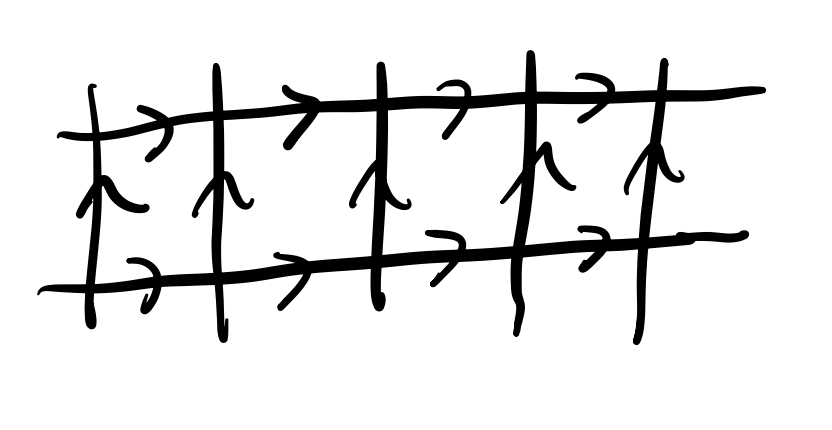
\includegraphics[scale=0.35]{Lectures/Images/lec7-orientation.png}
    \end{center}
    
    Now every star has 2 outgoing and 2 incoming arrows. So, let's work out what $A_g(s)$ in the outgoing case:

    \begin{center}
        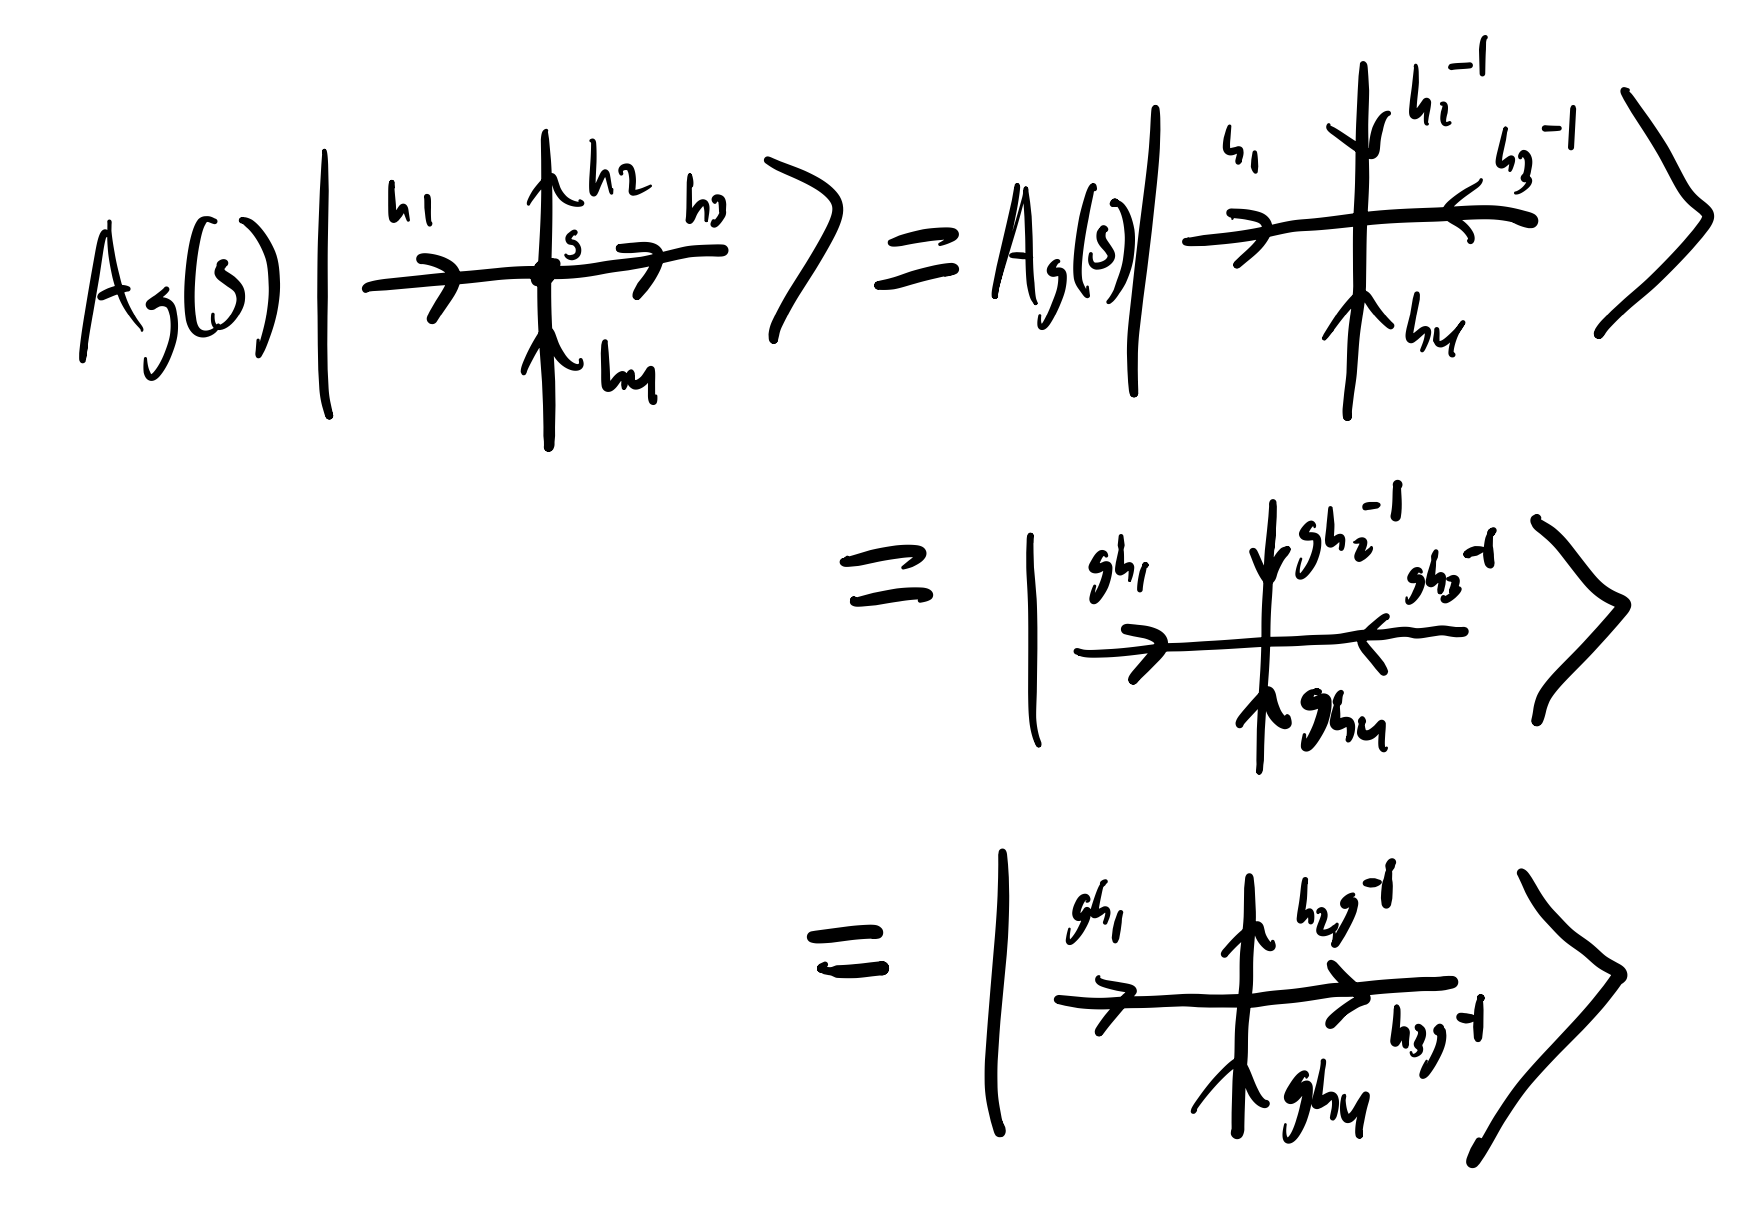
\includegraphics[scale=0.3]{Lectures/Images/lec7-Agreverse.png}
    \end{center}

    wherein in the second equality we flip the outgoing arrows so that we may apply our known action for $A_g(s)$ on incoming arrows, and in the last equality we flip again. Thus, in summary, $A_g(s)$ acts on left multiplication of $g$ on incoming arrows, and right multiplication of $g^{-1}$ on outgoing arrows.

    Now, it is easy to see that the star operators commute. We only need worry if the star operators overlap (if they don't overlap, they trivially commute):

    \begin{center}
        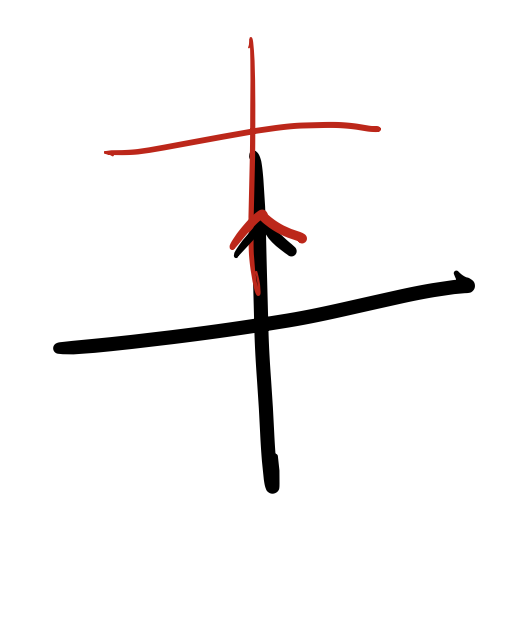
\includegraphics[scale=0.35]{Lectures/Images/lec7-staroverlap.png}
    \end{center}

    but then one will have a incoming arrow, one has an outgoing arrow (note this is true independent of any choice of orientation!). Since left and right multiplication commute, $[A_g(s), A_h(s')] = 0$ if $s \neq s'$ (if on the same site $gh \neq hg$ in general). Thus, $[A(s), A(s')] = 0$ for all $s, s'$ (the case where $s = s'$ is trivial in this case - its the same operator!)

    \item $[B(p), B(p')] = 0$ is obvious; they are all diagonal in the group element basis.
    
    \item First, we determine how to calculate the action of plaquette operator for this orientation:

    \begin{center}
        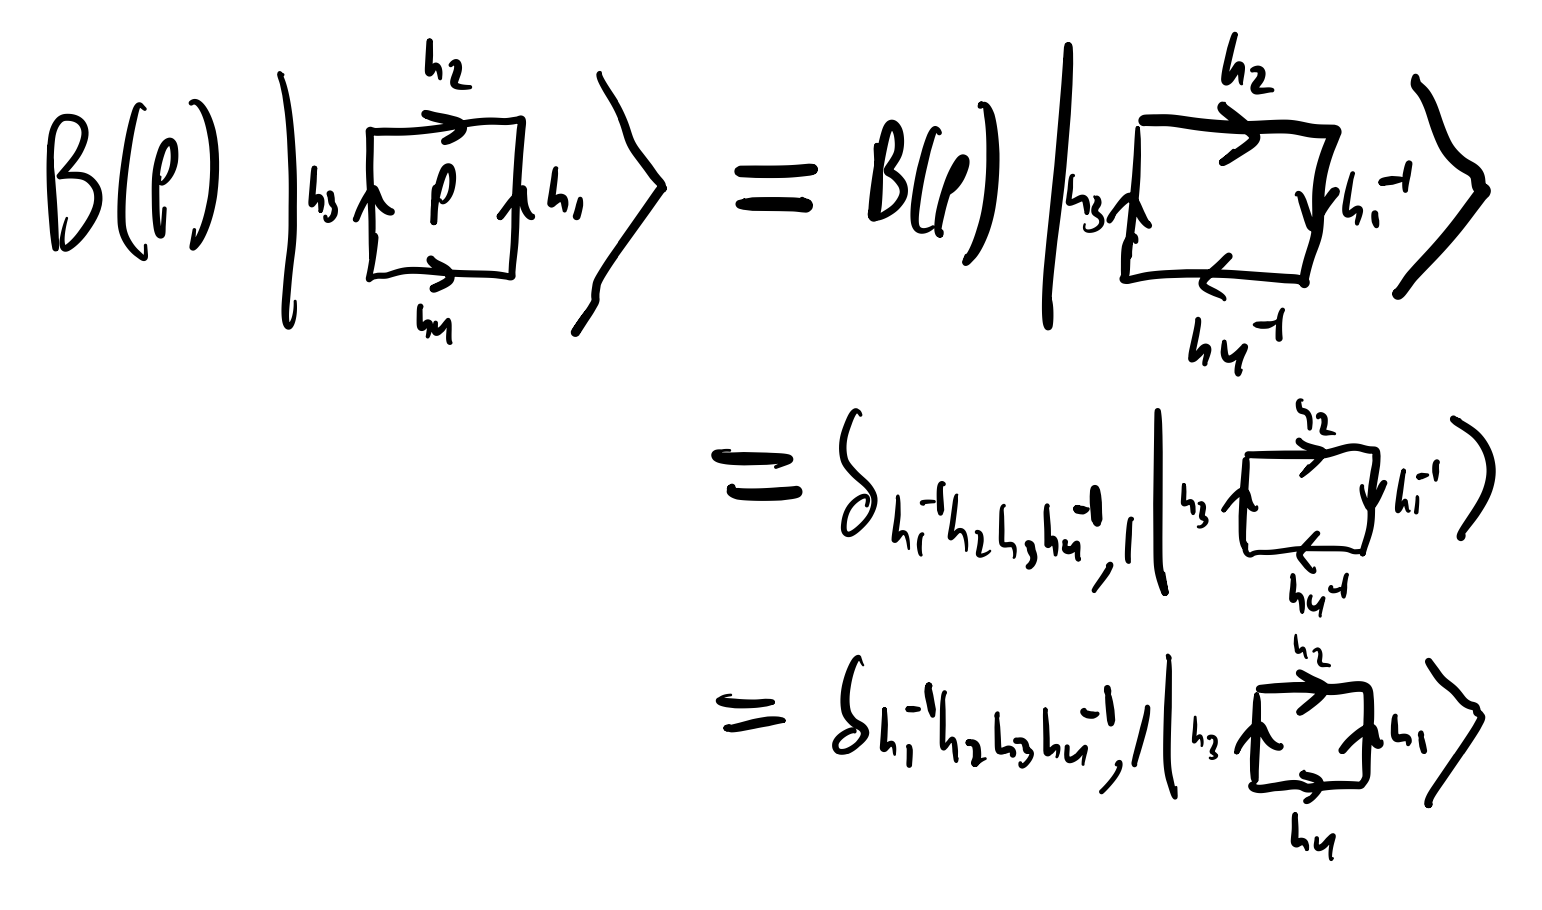
\includegraphics[scale=0.3]{Lectures/Images/lec7-Breverse.png}
    \end{center}

    where we can see if that we go against the arrow, we multiply by the inverse of the group element in the kronecker delta instead.
    
    Now for the commutation argument. If the star and plaquette have no overlap the commutation is trivial. What about when they do overlap? We have 4 cases to check. For when they overlap at the top right corner, the $A_g$ left and right multiplies in a way such that things cancel:

    \begin{center}
        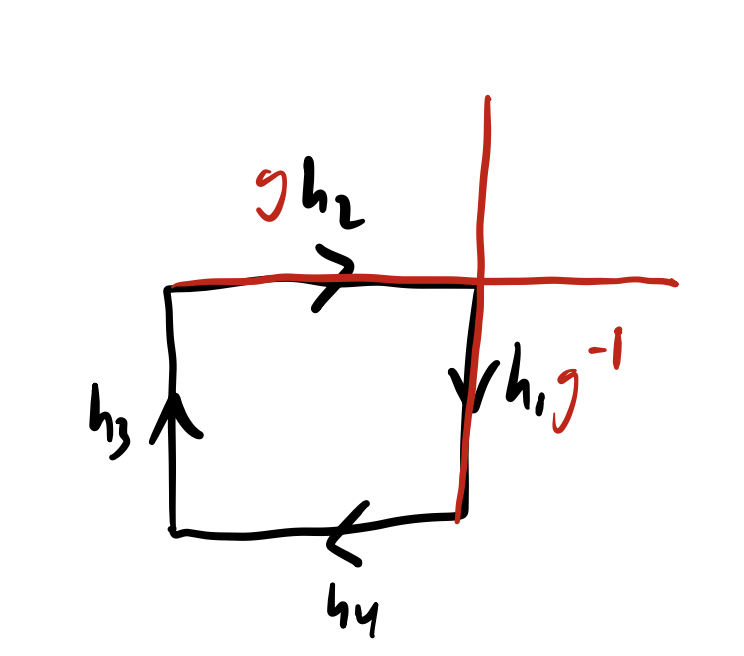
\includegraphics[scale=0.35]{Lectures/Images/lec7-overlap1.png}
    \end{center}

    \begin{equation}
        h_1h_2h_3h_4 \stackrel{A_g}{\to} (h_1g^{-1})(gh_2)h_3h_4 = h_1h_2h_3h_4
    \end{equation} 

    For the case when they overlap at the top left corner:

    \begin{center}
        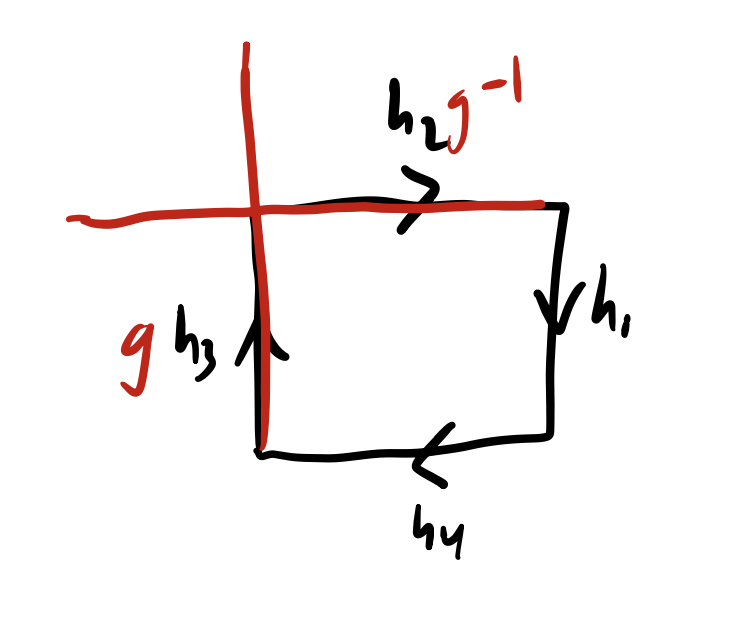
\includegraphics[scale=0.35]{Lectures/Images/lec7-overlap2.png}
    \end{center}

    \begin{equation}
        h_1h_2h_3h_4 \stackrel{A_g}{\to} h_1(h_2g^{-1})(gh_3)h_4 = h_1h_2h_3h_4
    \end{equation}

    the bottom left corner is exactly the same. The most interesting case is the bottom right corner; this is interesting case because this is our chosen basepoint from which we are measuring the flux:

    \begin{center}
        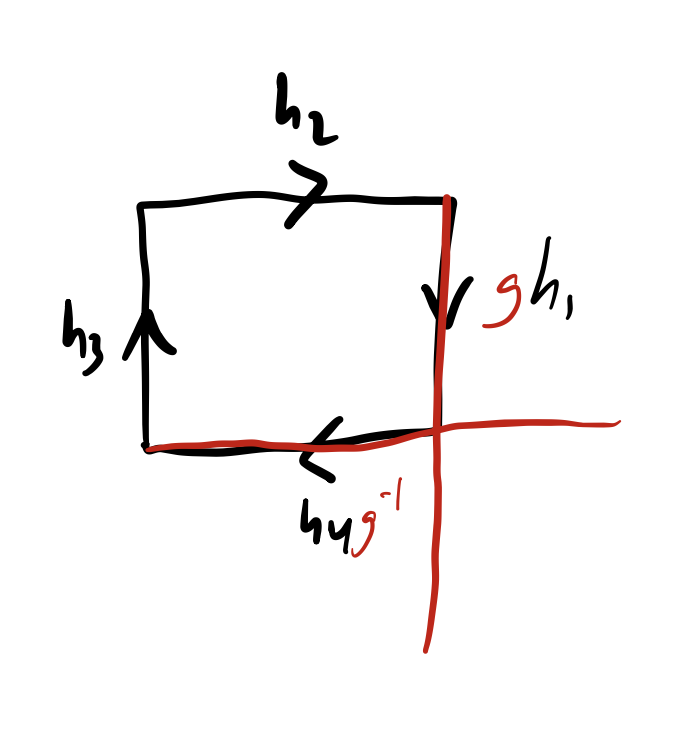
\includegraphics[scale=0.35]{Lectures/Images/lec7-overlap3.png}
    \end{center}

    \begin{equation}
        h_1h_2h_3h_4 \stackrel{A_g}{\to} (gh_1)h_2h_3(h_4g^{-1}) = g(h_1h_2h_3h_4)g^{-1}
    \end{equation}
    So $A_g$ conjugates the flux via a group element $g$ in this last interesting case. So, in all cases $A_g$ always preserves the conjugacy class of the flux $h_1h_2h_3h_4$. Thus:
    \begin{equation}
        [A_g(s), B(p)] = 0
    \end{equation}
    as 1 (and 0) are invariant under conjugation. Thus $[A(s), B(p)] = 0$.
\end{enumerate}

\subsection{Solution to the Quantum Double Model}
Since $\set{A(s), B(p)}$ are commuting projectors, i.e. have eigenvalues $0,1$, the ground states correspond to states $\ket{\Omega}$ with:
\begin{equation}
    A(s)\ket{\Omega} = B(p)\ket{\Omega} = \ket{\Omega}
\end{equation}
Our central question to answer is how many states $\ket{\Omega}$ that satisfy the above?

We consider the infinite plane geometry. From the Euler characteristic we intuit that there is a unique ground state in this case. We work in the $\ket{g}$ basis. Then:
\begin{equation}
    B(p)\ket{\Omega} = \ket{\Omega}
\end{equation}
implies that $\ket{\Omega}$ is a sum of states with ``vanishing flux'', i.e. $h_1h_2h_3h_4 = 1$. for example, on a very small lattice:

So there are many states with vanishing flux, and we can of course take linear combinations of them, so we have a linear combination with undetermined coefficients. But, we will then find that the constraint that $A(s) = 1$ everywhere enforces that all of the coefficients to be equal weight.

\begin{center}
    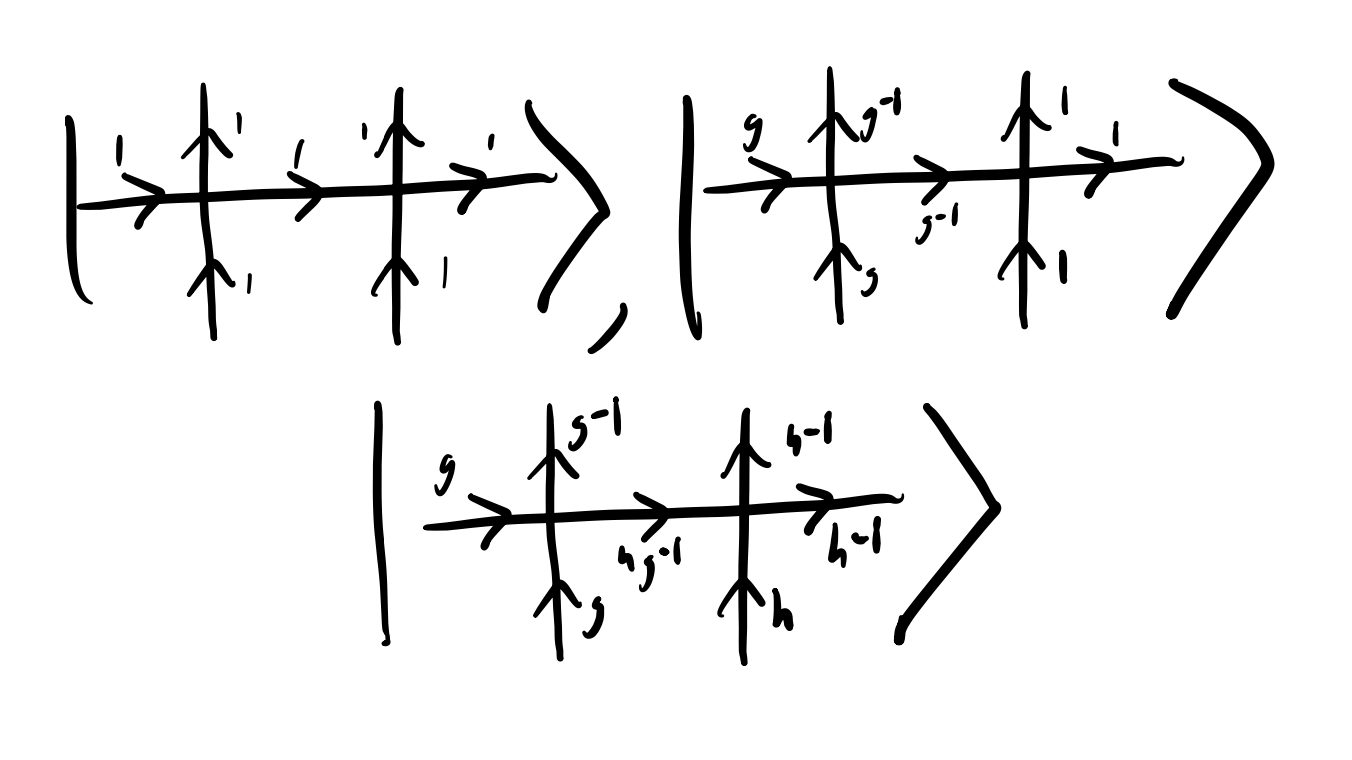
\includegraphics[scale=0.35]{Lectures/Images/lec7-nofluxstates.png}
\end{center}
\section{Topological quantum computation}
\section{Quantum Double Model IV}

\subsection{Review - Flux Excitations in QD Model}
Last time, we introduced the idea that there is one type of flux excitation for every non-trivial conjugacy class $C \subseteq G$. We constructed the explicit states:
\begin{equation}
    \ket{C} = \sum_{\set{g_j}}\ket{\set{g_j}}
\end{equation}
with $\set{g_j}$ such that we have flux $C$ through plaquette $p_0$ and 1/no flux elsewhere. This is analogous to the ground state of the original Hamiltonian, except we enforce the condition where there is a nontrivial flux through one plaquette.

In arguing for this, we explained how anyons should be the unique ground state of a trapping potential. In particular, the $\ket{C}$ above is the unique ground state of:
\begin{equation}
    H = -\sum_s A(s) - \sum_{p\neq p_0}B(p) - B_C(p_0)
\end{equation}
with $B_C(p)$ defined as:
\begin{center}
    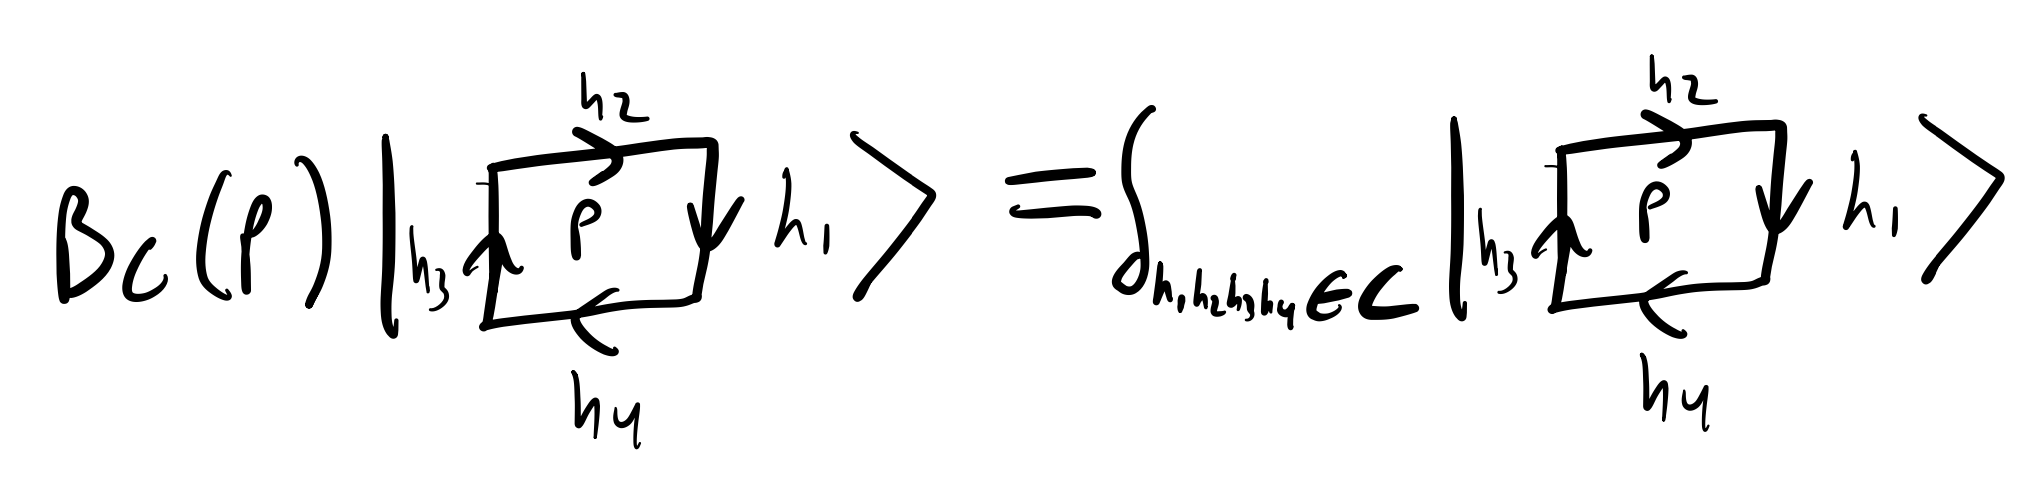
\includegraphics[scale=0.35]{Lectures/Images/lec8-Bcp.png}
\end{center}
Note that the $H$ above is a commuting projector Hamiltonian ,as $B_c(p_0)$ commutes with all the other terms. We showed that this is indeed the unique eigenstate by arguing that $B_C(\gamma)$ for a sufficiently large loop $\gamma$ around the flux can detect it, but must commute with any local operator around such a flux.

\subsection{Multiple Fluxes in QD Model}
We can easily generalize the above trapping Hamiltonian to that which traps several fluxes:
\begin{equation}
    H = -\sum_s A(s) - \sum_{p \neq p_1, \ldots p_n}B(p) - \sum_{i=1}^n B_{C_i}(p_i)
\end{equation}
\begin{center}
    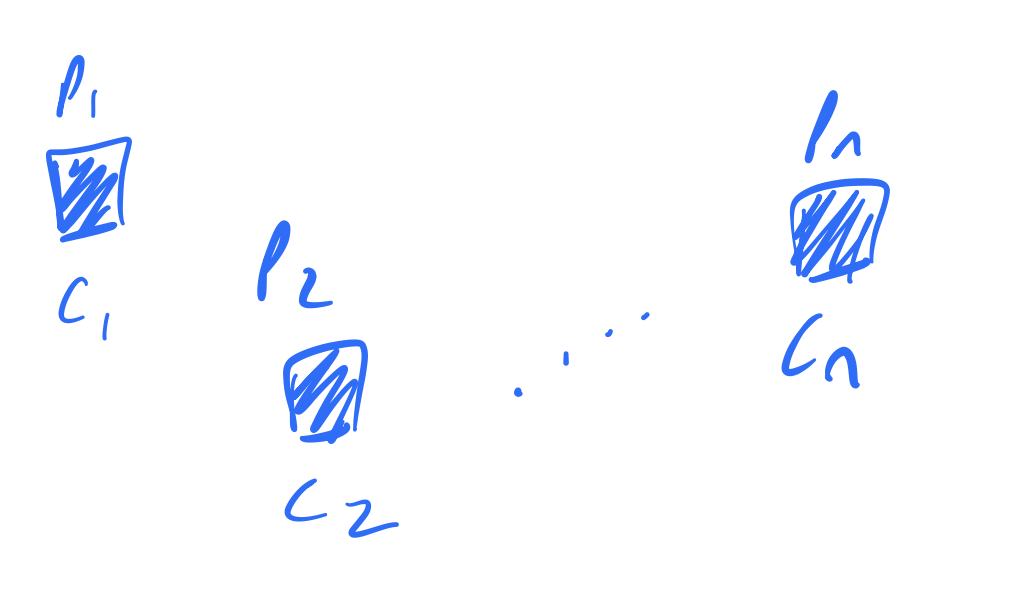
\includegraphics[scale=0.35]{Lectures/Images/lec9-multiplefluxes.png}
\end{center}

interestingly, we will find that in general $H$ has multiple degenerate ground states. To construct them, we choose different group elements in the different conjugacy classes, $g_i \in C_i$, with the constraint:

\begin{equation}
    g_1g_2 \ldots g_n = 1
\end{equation}
This constraint corresponds to ground states having trivial topological charge (and corresponds to the ability to create the ground state via a local term) - we will come back to this. We now construct the ground states in two steps. First, define the basis states:
\begin{center}
    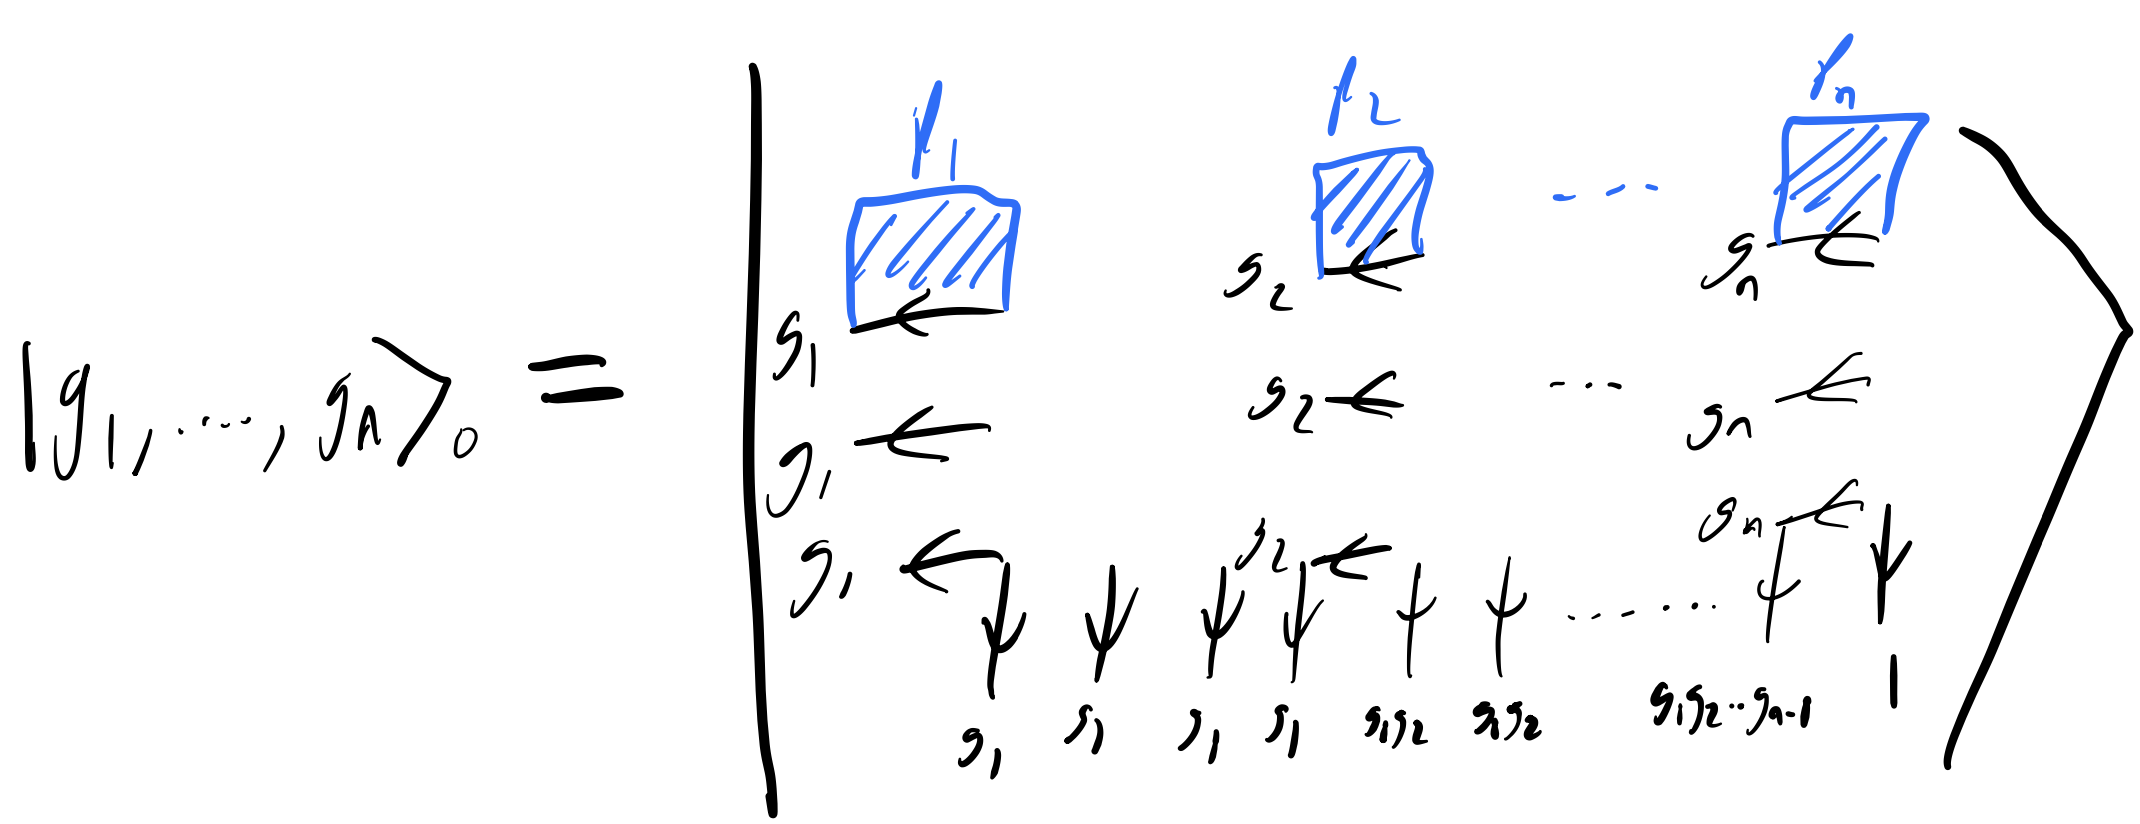
\includegraphics[scale=0.35]{Lectures/Images/lec9-naughtstates.png}
\end{center}
which produces the fluxes at the desired locations, and then we have branch cuts of non-trivial group elements on links such that all other fluxes are trivial ($g_i$ on the vertical columns, and then $g_1 \ldots g_{i-1}$ on the horizontal sections).

By construction, the flux through each $p_i$ is $g_i \in C_i$:
\begin{equation}
    B_c(p_i)\ket{g_1, \ldots g_n}_0 = \ket{g_1, \ldots g_n}_0
\end{equation}
and the flux through all other plaquettes is also 1:
\begin{equation}
    B(p)\ket{g_1, \ldots g_n}_0 = \ket{g_1, \ldots g_n}_0 \quad p \neq p_1, \ldots p_n
\end{equation}
So, so far the plaquette operators likes this state. But the star operators may not. We define the actual ground state to be:
\begin{equation}
    \ket{g_1, \ldots g_n} = \prod_s A(s)\ket{g_1, \ldots g_n}_0
\end{equation}
which is the projection to the $(s) = 1$ subspace. To get a flavour for what the projection does, we remember the definition of $A(s)$ as a sum of $A_g(s)$s; so:
\begin{equation}
    \ket{g_1, \ldots, g_n} = \prod_s\left(\frac{1}{\abs{G}}\sum_g A_g(s)\right)\ket{g_1, \ldots g_n}_0
\end{equation}
So it sums over all possible configurations that can be obtained by $\ket{g_1, \ldots g_n}_0$ via $A_g(s)$s. Because we have now projected into the $A(s) = 1$ subspace (note; there is no fear that the $A(s)$ could destroy the state, because they only have positive matrix elements), by construction these states will be eigenstates of $A(s)$:
\begin{equation}
    A(s)\ket{g_1, \ldots g_n} = \ket{g_1, \ldots, g_n}
\end{equation}
and because all of the terms in the Hamiltonian commute, the fact that these are still eigenstates of the $B$ operators does not change:
\begin{equation}
    B(p)\ket{g_1, \ldots g_n} = \ket{g_1, \ldots g_n} \quad p \neq p_1, \ldots p_n
\end{equation}
\begin{equation}
    B_{C_i}(p_i)\ket{g_1, \ldots g_n} = \ket{g_1, \ldots g_n}
\end{equation}
so indeed, $\ket{g_1, \ldots g_n}$ are eigenstates of every operator in $H$ with eigenvalue $+1$, so these are indeed ground states of $H$.

A side note; we could write the initial state $\ket{C}$ in this language, just imagining that the cut of non-trivial edges goes off to $\infty$.

\subsection{Ground states - redundancy and completeness}
So, we've found some ground states. But these states are actually not all distinct, there is some redundancy. This is because:
\begin{equation}
    \ket{g_1, g_2, \ldots, g_n} = \ket{hg_1h^{-1}, hg_2h^{-1}, \ldots, hg_nh^{-1}}.
\end{equation}
To see this, we note that the $\ket{g_1, g_2, \ldots, g_n}_0$ states are related by a uniform gauge transformation.
\begin{equation}
    \prod_s A_h(s)\ket{g_1, g_2, \ldots, g_n}_0 = \ket{hg_1h^{-1}, hg_2h^{-1}, \ldots, hg_nh^{-1}}_0
\end{equation}
This is evident from looking at the pictorial definition of the $\ket{g_1, g_2, \ldots, g_n}_0$ states. Indeed, every link gets conjugated by $h$:

\begin{center}
    \includegraphics[scale=0.35]{Lectures/Images/lec9-gauging.png}
\end{center}

Because the unprojected states are related by a gauge transformation , when we project onto all the $A(s)$s (and sum over all gauge equivalent combinations) we get the same answer. To see this formally:
\begin{equation}
    \begin{split}
        \ket{hg_1h^{-1}, hg_2h^{-1}, \ldots, hg_nh^{-1}} &= \prod_s\left(\frac{1}{\abs{G}}\sum_g A_g(s)\right)\ket{hg_1h^{-1}, hg_2h^{-1}, \ldots, hg_nh^{-1}}_0
        \\ &= \prod_s\left(\frac{1}{\abs{G}}\sum_g A_g(s)\right)\prod_{s}A_h(s) \ket{g_1, g_2, \ldots, g_n}_0
        \\ &= \prod_{s}\left(\frac{1}{\abs{G}}\sum_g A_g(s)A_h(s) \right)\ket{g_1, g_2, \ldots, g_n}_0
        \\ &= \prod_{s}\left(\frac{1}{\abs{G}}\sum_g A_{gh}(s) \right)\ket{g_1, g_2, \ldots, g_n}_0
        \\ &= \prod_s \left(\frac{1}{\abs{G}}\sum_g A_g(s)\right)\ket{g_1, \ldots, g_n}_0
        \\ &= \ket{g_1, \ldots g_n}
    \end{split}
\end{equation}
where we have used that the group maps to itself under multiplication in the second to last step.

It is not hard to see that this is the only redundancy. Thus:
\begin{equation}
    \braket{g_1, \ldots, g_n}{g_1', \ldots g_n'} = \delta_{g_i' = hg_i h^{-1} \forall i} \quad \text{for some $h \in G$}
\end{equation}
The intuition is that only a uniform gauge transformation can map between the different $\ket{g_1, g_2, \ldots, g_n}_0$ states (else, we get a mismatch on the trivial links, no longer making them trivial). The ground states are sums over gauge configurations, and as such the gauge orbits of non-gauge equivalent $\ket{g_1, g_2, \ldots, g_n}_0$ must be non-overlapping and hence orthogonal.

The punchline: There is a distinct ground state for every $(g_1, \ldots, g_n)$ (ordered list) with $g_1g_2\ldots g_n = 1$ (allowing this state to be created locally), modulo uniform conjugation.

The next question we can ask is - are these all of the ground states? The answer is yes, at least in a sense. These are all the ground states that can be created from $\ket{\Omega}$ (the GS of the original QD model) via an operator acting in a finite region, i.e. around $p_1, \ldots p_n$. It should be clear that we can create these states locally, the converse (that these states consist of all such states) has not been shown explicitly, but is true. In other words, these are the full set of all ground states with trivial ``total topological charge''.

\subsection{Ground state properties}
We label distinct $\ket{g_1, \ldots g_n}$ states by:
\begin{equation}
    \set{\ket{\alpha}, \alpha = 1, \ldots D}
\end{equation}
\begin{enumerate}
    \item There is an exponentially large ground state degeneracy if conjugacy classes have more than one element. For example take $G = S_3 = \set{\II, (12), (13), (23), (123), (132)}$. We have three conjugacy classes:
    \begin{equation}
        C_1 = \set{\II}, \quad C_2 = \set{(12), (13), (23)}, \quad C_3 = \set{(123), (132)}
    \end{equation}
    For $C_2$, we have:
    \begin{equation}
        D_n = \frac{3^{n-1} + 3}{6}
    \end{equation}
    with $n$ - the number of fluxes - here even (you can verify that for $C_2$, no odd number of fluxes can multiply to the identity, as we require).

    More generally, if all $C_i = C$, then:
    \begin{equation}
        D_n \sim \abs{C}^n \cdot \text{const.} \text{ as $n \to \infty$}
    \end{equation}

    \item The ground states are locally indistinguishable. For any $O$ supported on less than $L$ sites where $L = \min_{i, j} \text{dist}(p_i, p_j)$, then:
    \begin{equation}
        \bra{\alpha}O\ket{\beta} = c\delta_{\alpha\beta}
    \end{equation}
    Suppose we have $\ket{g_1, \ldots, g_n}, \ket{g_1', \ldots, g_n'}$. So we might say that there is the ability to distinguish at $p_1$. But for any given flux, I can via conjugation make the flux at $g_1$ look the same $g_1' \to h g_1' h^{-1} = g_1$. So, we need to be able to see more than one flux.

    \item The ground state degeneracy is robust to small local perturbations of $H$. If we take $H \to H + \lambda V$, the splitting is $\delta \sim e^{-\text{const.}L}$. Roughly (as in the toric code case) it follows from property 2, where we need order $L$ perturbation theory to connect states in the ground space.
\end{enumerate}

One last comment - we see the above features, and these are all generic/defining features of non-abelian anyons. Next time, we will look more closely at the non-Abelian nature of these objects, and braid the non-Abelian anyons and look at their braid matrices.
\section{AKLT model}
\section{Topological Quantum Computation, Gapped Phases of Matter}
Over the last few lectures, we have discussed Non-abelian anyons in the quantum double model and their properties. We looked at their braiding properties as well as the projective measurement of their total topological charge. These two ideas, when put together, allow us to carry out a quantum computation using Non-abelian anyons. This is a very elegant and new approach. The first proposal by Kitaev was in the context of the quantum double model, so this is where we too shall discuss it.

\subsection{The ingredients}
Consider the QD model for some non-abelian group $G$. Assume that we can perform the following operations:
\begin{enumerate}
    \item We can create pairs of fluxes of each ``type'', i.e. for each nontrivial conjugacy class.
    \item We can braid pairs of (nearby) fluxes.
    \begin{center}
        \includegraphics[scale=0.35]{Lectures/Images/lec11-swap.png}
    \end{center}
    \item We can measure $B_1(\gamma)$ for any pair of fluxes:
    \begin{center}
        \includegraphics[scale=0.35]{Lectures/Images/lec11-loop.png}
    \end{center}
    Physically, we can measure this by taking charge excitations and braiding them around the loop. So, we could replace this stipulation with the ability to braid charges around fluxes.
    \item We can measure whether a pair of fluxes has trivial total topological charge. For this, we need to braid both charges and fluxes (and both have to be trivial). Physically we could imagine this as some adiabatic evolution.
\end{enumerate}
3 is a subset/coarser measurement than 4. It only measures whether the braid with charges is trivial. 4 measures whether the braid with both charges and fluxes are trivial. Note that we do not need to know \emph{what} the flux is, only whether it is trivial or not.

The claim: If $G$ is a simple (that is, $G$ does not have any nontrivial normal subgroup, where normal means to be preserved under conjugation) non-abelian group, then we can use efficiently simulate (there is a constant overhead to simulate each gate in the universal gateset via braiding) any quantum circuit with these operations.

\begin{center}
    \includegraphics[scale=0.35]{Lectures/Images/lec11-qcircuit.png}
\end{center}

As an example, the smallest simple non-abelian group is $A_5$ (even permutations of 5 elements), with 60 elements. Note that this result has been extended, to smaller groups, e.g. $S_3$.

\subsection{Idea}
Consider $N$ fluxes. 
\begin{center}
    \includegraphics[scale=0.35]{Lectures/Images/lec11-Nfluxes.png}
\end{center}

There is an exponentially large degeneracy $\sim \abs{C}^N$. It turns out that we can define a convenient subspace (sometimes called the computational subspace) of dimension $2^{N/2}$. This allows us to represent $N/2$ qubits. Specifically, choose two elements $a, b \in G$, with $b^2 = 1$ and $ab \neq ba$ (for a non-abelian simple group, we can always find such $a, b$). Define:
\begin{center}
    \includegraphics[scale=0.35]{Lectures/Images/lec11-compbasis.png}
\end{center}
A typical computational state (say $\ket{0100\ldots}$) then looks like:
\begin{center}
    \includegraphics[scale=0.35]{Lectures/Images/lec11-basisstateexample.png}
\end{center}

Note that there are a few ancillary fluxes\footnote{John Preskill calls this the ``flux bureau of standards''.} which fixes the issue of uniform conjugation which maps $\ket{0} \leftrightarrow \ket{1}$ - these ancillary fluxes are the ``reference fluxes'' which allow us to tell apart $\ket{0}$ and $\ket{1}$.

If the group is simple, we can perform the Toffoli gate - a particular 3 qubit gate - using braiding. Note that this is a classical gate universal for classical computation. Further, we can apply and measure single qubit Paulis $X,Y,Z$. 

Measuring $Z$ is simple; if we have a reference flux (say, $a$), we can measure $B_1(\gamma)$ around the reference flux and one half of the pairs of fluxes that make up $\ket{0}$ or $\ket{1}$. For $\ket{0}$ we find the flux is trivial and for $\ket{1}$ we find the flux is nontrivial.

Measuring $X$ has to do with measuring the total topological charge. If we are in the state $\ket{0} - \ket{1}$, we have a state which is orthogonal to the state which has trivial total topological charge, because $\ket{0}, \ket{1}$ have trivial total topological charge, and only a symmetric combination of these will have trivial total topological charge.

Then $\set{\text{Toffoli}, X, Y, Z}$ is a universal gate set for quantum computation, so we are done! For details, see John Preskill's lecture notes on quantum computation (Chapter 9.11) \url{http://theory.caltech.edu/~preskill/ph219/topological.pdf}.

We don't go through the gory details of this particular protocol, but we do comment that one can prove a similar result for many other types of non-Abelian anyons.

What is the advantage of this kind of model of QC? It is naturally protected against decoherence and errors, so long as anyons are far apart during braiding and measurement (and you work at sufficiently low temperature). In some sense, the quantum error correction is already baked in at the hardware level. This comes from the fact that the system is robust to local perturbations.

\subsection{Defining gapped phases of matter}
Thus far, we have been focusing on very specific models. But we may wonder to the extent to which the properties we have seen are general/persistent, e.g. under perturbations. To discuss this, we want to introduce the notion of a gapped phase of matter.

The setting will be qubits on a lattice with local interactions and an energy gap. What do we mean by ``local'' or ``short-range''? The rough definition is that:
\begin{equation}
    H = \sum_r H_r
\end{equation}
where $H_r$ is supported within a finite distance of $r$.

\begin{center}
    \includegraphics[scale=0.35]{Lectures/Images/lec11-localH.png}
\end{center}

Strictly speaking, we will allow for something slightly more general. Instead of only allowing for strictly short range interactions, we will allow for interactions that decay super-polynomially (faster than any power law):
\begin{equation}
    \norm{[H_r, O_{r'}]} \leq \mathcal{O}(\abs{r - r'}^{-\infty})
\end{equation}
where $\leq \mathcal{O}(\abs{r - r'}^{-\infty})$ means $\leq \frac{C}{\abs{r - r'}^n}$ for any $n$, $O_{r'}$ is some single-site operator at $r'$, and $\norm{\cdot}$ is the operator norm. The classic example is exponentially decaying tails.

By energy gap, we mean that in the thermodynamic limit (system size $\to \infty$) we have a finite energy between the ground state(s) and the excited states of the system.

\textit{Definition.} Two local, gapped Hamiltonians $H_a, H_b$ belong to the same phase if there exists an interpolating family of Hamiltonians $\set{H(s): 0 \leq s \leq 1}$ with $H(0) = H_a, H(1) = H(b)$ such that $H(s)$ is local and gapped for all $s$.

\begin{center}
    \includegraphics[scale=0.35]{Lectures/Images/lec11-interpolation.png}
\end{center}

Two comments about the definition:
\begin{itemize}
    \item Analogy with the finite $T$ definition of phases. Recall the phase diagram of water:

    Here, two points are in the same phase so long as we can find a path connecting them such that the free energy is smooth/analytic along the path (at the phase transition, we have a non-analyticity). This idea of two points in a phase being connected by a ``nice'' path is analogous.

    \begin{center}
        \includegraphics[scale=0.35]{Lectures/Images/lec11-water.png}
    \end{center}

    In the above diagram, two water points are in the same phase (path $A$). Water and steam are also in the same phase, as (going to high enough temperature) we can find a path that smoothly connects water and steam (path $B$). However, there is no path that connects ice with water without going through a phase transition, so these points must correspond to different phases. This points out one condition about the definition - it is easier to conclude that two things are in the same phase (because we need only find a single path that works) vs. things are in different phases (in which case we need to show that \emph{all} paths cannot work).
    \item The existence of an interpolation implies $H_a, H_b$ are adiabatically connected. We thus intuitively expect that $H_a, H_b$ have the same physical properties, since we are able to continuously deform one system into the other.
\end{itemize}
This was the status of phases of matter $> 20$ years ago. But around 2 decades ago, people developed a way to make this intuition more precise, using tools from quantum information.

\subsection{Local Unitary Transformations}
\emph{Definition.} A \emph{local unitary transformation} $U$ is any unitary that can be generated by the time evolution of a local Hamiltonian (with local as we definined previous - either finite range or superpolynomially decaying interactions) over a finite time $t$. In other words, we can write it as the time ordered exponential:
\begin{equation}
    U(T) = \mathcal{T}\exp(-i\int_0^T H(t)dt)
\end{equation}
where $H$ is local.

In what sense is this $U$ local? Generated by something local - certainly, but a priori we cannot measure this. The more physical thing we can measure is the fact that it maps local operators to local operators. This is a result due to Lieb and Robinson.

\textit{Theorem (Lieb-Robinson bound).} Let $U =  \mathcal{T}\exp(-i\int_0^T H(t)dt)$ with $H(t)$ local. Let $O$ be an operator supported in some region $R$. Then, $U^\dag O U$ is supported within distance $v_{LR}T$ of $R$, with superpolynomially decaying tails. $v_{LR}$ is the Lieb-Robinson velocity, and is determined by the range of interactions in $H(t)$.

\begin{center}
    \includegraphics[scale=0.35]{Lectures/Images/lec11-LRbound.png}
\end{center}

Some intuition; if we imagine calculating $U^\dag O U$ for time-independent $H$, we want to calculate something like $e^{iHT}Oe^{-iHT}$. We could then expand this out in a power series:
\begin{equation}
    e^{iHT}Oe^{-iHT} \approx O + iT[H, 0] - \frac{T^2}{2}[H, [H, O]] + \ldots
\end{equation}
wherein if $H$ has short range interactions, each commutator in the power series spreads $O$ slightly.

Next time, we will use these concepts to show that two $H$ in the same phase have ground states that are related by a local unitary transformation.
\section{SPT phases II}
\section{Area law for entanglement entropy in gapped systems}
\section{Entanglement entropy in gapless systems}
\section{AKLT model, Entanglement Entropy I}
We discuss one more model of a 1-D SPT; the AKLT (Affleck-Kennedy-Lieb-Tasaki) model. This was (arguably) the first SPT phase that was understood.

\subsection{Defining the model}
We now consider a chain of qutrits/spin-1 particles.

\begin{center}
    \includegraphics[scale=0.35]{Lectures/Images/lec15-spinchain.png}
\end{center}

The Hamiltonian takes the form:
\begin{equation}
    H = \sum_i P_2(\v{S}_i + \v{S}_{i+1})
\end{equation}
what is this? This is a projection that acts on two neighbouring sites, and projects it onto states with total spin 2 (the projection onto the subspace with eigenvalues $s(s+1) = 2(2+1) = 6$).  This projector has a reasonably nice form:
\begin{equation}
    H = \sum_i \left[\frac{1}{2}\v{S}_i \cdot \v{S}_{i+1} +\frac{1}{6}(\v{S}_i\cdot\v{S}_{i+1})^2 + \frac{1}{3}\right]
\end{equation}
Note that any rotation-symmetric quantity can be written as a function of $\v{S}_i \cdot \v{S}_{i+1}$, which is what we see above. 

% There are three possible projectors we could write down, $P_0, P_1, P_2$, the third is not independent (is just $\II - P_i - P_j$) so this motivates why we just get the terms that we do.

We focus on the (global) $SO(3)$ symmetry of the model. Why is it a nontrivial phase in the presence of this symmetry? Let us write down a unitary operator for each rotation matrix in $SO(3)$:
\begin{equation}
    U(R(\theta, \hat{\v{n}})) = \prod_k e^{-i\theta \v{S}_k \cdot \hat{\v{n}}}
\end{equation}

Note that each site transforms under a linear (\emph{not} projective) representation of $SO(3)$. This is because they are spin-1 (this is the analog of each site of our cluster state transforming under a linear representation of $\mathbb{Z}_2 \times \mathbb{Z}_2$). When we look at the boundary, we will see that the symmetry acts on the boundary via projective representations\footnote{and this motivates why $SO(3)$ rather than $SU(2)$, as $SU(2)$ does not have projective representations.}

\subsection{Constructing the ground state}
One can show that $H$ has a unique ground state $\ket{\Omega}$ and a gap in infinite (or periodic) chain. This ground state has a simple picture; we represent each spin-1 as two spin-1/2s in a spin-triplet state:
\begin{equation}
    \begin{split}
        \ket{+} &\leftrightarrow \ket{\uparrow\uparrow}
        \\ \ket{0} &\leftrightarrow \frac{\ket{\uparrow\downarrow} + \ket{\downarrow\uparrow}}{\sqrt{2}}
        \\ \ket{-} &\leftrightarrow \ket{\downarrow\downarrow}
    \end{split}
\end{equation}
We have no singlet state - the singlet state for the spin-1/2s does not correspond to a physical state in the real spin-1 system. Why did we do this weird rewriting in terms of virtual spin-1/2s? The ground states will have a very simple form in this notation:

\begin{center}
    \includegraphics[scale=0.35]{Lectures/Images/lec15-AKLTGS.png}
\end{center}

The blue lines connecting the fictituous spin-1/2 particles on neighbouring sites corresponds to the projection onto the spin singlet state $\frac{\ket{\uparrow\downarrow} - \ket{\downarrow\uparrow}}{\sqrt{2}}$. This alone is not good, because we are taken out of the space of physical spin-1 states. So, after the singlet projection, we apply the black circles, which are a projection onto the spin-triplet subspace for each ``true'' spin-1 site.

To see that $\ket{\Omega}$ is indeed the ground state of $H$, note that we have a maximum spin of $1/2$ from each of the boundary spins, and then a spin of 0 from the singlet (note that this analysis seems like it happened before the triplet projection - but since the triplet projection is $SU(2)$ symmetric, it doesn't change the spin, so this is justified).

\begin{center}
    \includegraphics[scale=0.35]{Lectures/Images/lec15-AKLTspin.png}
\end{center}

To, the total spin of $i, i+1$ is bounded above by $\frac{1}{2} + 0 + \frac{1}{2} = 1$. So:
\begin{equation}
    P(\v{S}_i + \v{S}_{i+1})\ket{\Omega} = 0
\end{equation}
which allows us to indeed conclude that this is a ground state.

\subsection{Physics of the boundary}
Let's truncate the Hamiltonian to fit on our open chain:
\begin{equation}
    H = \sum_{i=1}^{N-1}P_2(\v{S}_i + \v{S}_{i+1})
\end{equation}
We can now see immediately that there are 4 degenerate ground states:

\begin{center}
    \includegraphics[scale=0.35]{Lectures/Images/lec15-AKLTboundary.png}
\end{center}

The boundary spins are now free to be up or down, and the same construction of singlet/triplet projection yields that all four choices of $\uparrow/\downarrow$ gives a ground state.

The degeneracy is just like the cluster state! The cluster state was a commuting projector Hamiltonian/solvable but less intuitive - here we have no commuting projector Hamiltonian but the picture is more intuitive/not solvable. But the physics is the same.

From the picture, it is clear that we have effective qubits on the left/right boundaries of the system (this interesting! We started with qutrits and now the effective DoFs are qubits), and that they transform like spin-1/2 under $SO(3)$. While spin-1 is a linear representation of $SO(3)$, spin-1/2 is a projective representation of $SO(3)$; we again see that the symmetry acts via projective representation on the boundaries of the system.

\subsection{Generalizations}

Note that there is a similar structure for other 1D (bosonic) SPT phases. The sites transform under a linear representation of $G$. But, when we define the system on an open chain, we get edge states that transform under a projective representation of $G$. The physical consequence of this structure is you get a robust GSD in an open chain.

We can also consider higher-dimensional SPT phases. For example, consider a 2D spin lattice with a boundary. In this case, we find that the symmetry action on the edge degrees of freedom is anomalous - roughly speaking, it means the symmetry acts in a way that is impossible to get for a lower-dimensional system. In 1-D the symmetry action at the boundary gave us GSD. In higher dimensions, it roughly gives us robust gapless modes; even though we may have a gap in the bulk at the boundary the gap closes.

\subsection{Schmidt Decomposition}
We now move to the last topic of the course, about entanglement measures. To this end let's review notions of the Schmidt decomposition and entanglement entropy.

Consider a state $\ket{\Psi}$ defined on a collection of qubits, partitioned into two subsets $A, A^c$.

\begin{center}
    \includegraphics[scale=0.35]{Lectures/Images/lec15-subsystems.png}
\end{center}

Then, the Schmidt decomposition of $\ket{\Psi}$ is:
\begin{equation}
    \ket{\Psi} = \sum_i \lambda_i \ket{\psi^i_A}\otimes \ket{\psi^i_{A^c}}
\end{equation}
for $\lambda_i \geq 0$. $\set{\ket{\psi^i_A}}_i, \set{\ket{\psi^i_{A^c}}}_i$ are orthonormal bases for $\mathcal{H}_A, \mathcal{H}_{A^c}$. Normalization tells us that:
\begin{equation}
    \sum_i \abs{\lambda_i}^2 = 1.
\end{equation}
We call the $\lambda_i$s Schmidt coefficients. These are unique up to reordering. We call the $\ket{\psi^i_A}, \ket{\psi^i_{A^c}}$ Schmnidt states, which are unique up to phases if the $\lambda_i$ are non-degenerate (in which case they would be unique up to unitary mixing of the states with the same Schmidt coefficient).

This all follows from singular value decomposition of matrices - same thing with a different name.

Note that $\set{\lambda_i}$ characterize the entanglement between $A, A^c$. We can see this from two properties:
\begin{enumerate}
    \item $\set{\lambda_i}$ are invariant under $\ket{\Psi} \to U_AU_{A^c}\ket{\Psi}$, where $U_{A}, U_{A^c}$ are unitaries that act on $A, A^c$ only. We can see that the unitary transformation would only change/rotate the basis of Schmidt states, but the coefficients would be preserved.
    \item $\set{\lambda_1 = 1, \text{others} = 0} \iff$ $\ket{\Psi}$ is a product state $\ket{\Psi} = \ket{\psi_A} \otimes \ket{\psi_{A^c}}$. Other values of $\lambda_i$ imply that the state is entangled.
\end{enumerate}

\subsection{Entanglement Entropy}
Let $\rho = \dyad{\Psi}{\Psi}$. Then, we define the Von Neumann entanglement entropy of $A$ as:
\begin{equation}
    S(\rho_A) = -\Tr(\rho_A\log \rho_A)
\end{equation}
where $\rho_A$ is the reduced density operator:
\begin{equation}
    \rho_A = \Tr_{A^c}(\rho)
\end{equation}
which is the reduced density operator.

Let's discuss the relationship between the Von Neumann entanglement entropy and the Schmidt coefficients $\set{\lambda_i}$. If we look at the expression for the Schmidt decomposition of $\ket{\Psi}$ across $A/A^c$ we can see that:
\begin{equation}
    \rho_A = \sum_i \abs{\lambda_i}^2\dyad{\psi^i_A}{\psi^i_A}
\end{equation}
The eigenvalues of $\rho_A$ are then $\set{\abs{\lambda_i}^2}$, and so:
\begin{equation}
    S(\rho_A) = -\sum_i \abs{\lambda_i}^2\log(\abs{\lambda_i}^2)
\end{equation}
indeed the entropy depends on the Schmidt coefficients, so $S(\rho_A)$ is indeed an entanglement measure. Because we get the same $\lambda_i$s whether we work with $A$ or $A^c$, an immediate (and intuitive) consequence is:
\begin{equation}
    S(\rho_A) = S(\rho_{A^c}).
\end{equation}

Properties of $S(\rho_A)$:
\begin{enumerate}
    \item $S(\rho_A)$ is invariant under $\rho \to U_A U_{A^c} \rho U^\dag_{A^c}U_{A^c}$ which is clear because it depends on the $\set{\lambda_i}$s, which are invariant under such a unitary that does not cross the bipartition.
    \item $S(\rho_{A_1} \otimes \rho_{A_2}) = S(\rho_{A_1}) + S(\rho_{A_2})$ for regions $A_1, A_2$.
    \item $0 \leq S(\rho_A) \leq \log(\text{min}(\dim \mathcal{H}_A, \text{dim} \mathcal{H}_{A^c}))$, where $\text{dim} \mathcal{H}_A$ is the dimension of the Hilbert space associated with $A$. This is achieved by setting all of the Schmidt coefficients to be equal weight (and corresponds to the maximally mixed state).
    \item $S(\rho_A) = 0 \iff \ket{\Psi} = \ket{\psi_A} \otimes \ket{\psi_{A^c}}$, $S(\rho_A) \neq 0 \iff \ket{\Psi}$ entangled.
    \item $S(\rho_{AB}) + S(\rho_{BC}) \geq S(\rho_{ABC}) + S(\rho_B)$ for any regions $A, B, C$ with $AB = A\cup B, BC = B \cup C$, $ABC = A \cup B \cup C$. This is the strong subadditivity property, and a very deep and nontrivial result, and motivates this entanglement measures over other ones.
\end{enumerate}

Next class we will discuss entanglement entropy in many-body systems.
\section{Entanglement Entropy II}

\subsection{Review of Entanglement entropy}
Given $\rho = \dyad{\psi}{\psi}$, we can partition the set of qubits which $\rho$ lives on into two subsets $A, A^c$. We can then define the Von Neumann entanglement entropy:
\begin{equation}
    S(\rho_A) = -\Tr(\rho_A\log \rho_A)
\end{equation}
with $\rho_A$ the reduced density operator:
\begin{equation}
    \rho_A = \Tr_{A^c}(\rho)
\end{equation}
this has some nice properties:
\begin{enumerate}
    \item $S(\rho_A) = S(\rho_{A^c}) = -\sum_i \abs{\lambda_i}^2\log(\abs{\lambda_i}^2)$ with $\lambda_i$ the Schmidt coefficients discussed last class.
    \item $S$ measures entanglement between $A, A^c$, with $S(\rho_A) = 0 \iff \ket{\psi} = \ket{\psi_A} \otimes \ket{\psi_B}$. Conversely, $S(\rho_A) \neq 0 \iff \ket{\psi} \text{is entangled}$.
\end{enumerate}

The absolute simplest example is for the Bell pair, or singlet state:
\begin{equation}
    \ket{\psi} = \frac{1}{\sqrt{2}}(\ket{\uparrow}_A\otimes \ket{\downarrow}_{A_c} - \ket{\downarrow}_A \otimes \ket{\downarrow}_{A_c})
\end{equation}
This is basically already written in terms of a Schmidt decomposition, just need to make the coefficients positive:
\begin{equation}
    \ket{\psi} = \frac{1}{\sqrt{2}}\ket{\uparrow}_A \otimes \ket{\downarrow}_{A^c} + \frac{1}{\sqrt{2}}\ket{\downarrow}_A \otimes (-\ket{\uparrow}_{A^c})
\end{equation}
so $\lambda_1 = \lambda_2 = \frac{1}{\sqrt{2}}$. The entanglement entropy is thus:
\begin{equation}
    S(\rho_A) = \log(2)
\end{equation}
in information theory the convention of base-2 logarithms is often used, but let us just write things using the natural log here. Roughly, we can think of $S(\rho_A)$ to be measuring the number of Bell pairs that are shared across $A$ and $A^c$.

\subsection{Scaling of entanglement entropy in gapped ground states}
The setting has been thus far for very general quantum systems. Now, we ask about the entanglement properties of ground states of local Hamiltonians. The best understood case is gapped ground states, which we will talk about now. 

Let $\ket{\psi}$ be the unique ground state of a gapped finite-range Hamiltonian $H$ defined on an infinite $d$-dimensional lattice. Let $A$ be a finite subset:

\begin{center}
    \includegraphics[scale=0.35]{Lectures/Images/lec16-Aregion.png}
\end{center}

The most basic question we can ask is how does $S(\rho_A)$ scale with $A$? This is not just a curiosity, but also has some practical implications - the scaling can have implications for ease of classical simulation.

This is generically a difficult question to answer. It has not been answered except in some special cases. But there is a hand-wavey intuition for what the answer should be, as well as many examples where it has been calculated.

The intuition proceeds as follows. Gapped states have short-range correlations (follows from Lieb-Robinson bounds; we also saw it during the discussion of anyons). More precisely:
\begin{equation}
    \bra{\psi}O_1O_2\ket{\psi} = \bra{\psi}O_1\ket{\psi}\bra{\psi}O_2\ket{\psi} + \text{exponentially small quantity in $\text{dist}(O_1, O_2)$}
\end{equation}
We could equivalently say this as the connected correlator:
\begin{equation}
    \avg{O_1O_2}_c = \avg{O_1O_2} - \avg{O_1}\avg{O_2}
\end{equation}
is exponentially small in the distance between $O_1, O_2$. In a rough sense, there is an exponential supression of singlets across long distances. There is only singlets/entangelment on short distances.

Hence - we expect (handwavey jump) that only degrees of freedom near the boundary of $A$ are entangled with $A^c$.

\begin{center}
    \includegraphics[scale=0.35]{Lectures/Images/lec16-perimeterlaw.png}
\end{center}

So we thus expect that $S(\rho_A) \propto \text{length/area}$ of the boundary. We call this ``area law'' scaling (coming from 3D; the boundary of a volume has an area).

Question - can an operation on one subset change the entanglement across the boundary? Sometimes we use the probe of mutual information which is monotonic under local operations $I(A:B) = S(\rho_A) + S(rho_B) - S(\rho_{AB})$ which for pure states is just $2S(\rho_A)$.

\subsection{Area law conjecture}
\emph{Area law conjecture.} If $\ket{\psi}$ is the unique gapped ground state of a finite range Hamiltonian $H$, then:
\begin{equation}
    S(\rho_A) \leq C\abs{\p A}
\end{equation}
Where $\abs{\p A}$ is the number of edges o the lattice that connect $A, A^c$, i.e. the length/area of the boundary of $A$. $C$ is some constant that depends only on $\ket{\psi}$, not on $A$.

A few comments about this inequality:
\begin{enumerate}
    \item The maximum possible value of $S(\rho_A) = \abs{A}\log(\dim(\mathcal{H}_{site}))$, e.g. $N\log(2)$ for a region of $N$ qubits, for example. This maximum follows from the Schmidt decomposition; the maximum number of Schmidt states we could have is $\dim(\mathcal{H}_A) = \dim(\mathcal{H}_{\text{site}})^{\abs{A}}$, and the maximum entropy we could have is the logarithm of this. Pictorially, the maximum entanglement is for each site in $A$ to be entangled with something on the outside. In other words, the entanglement scales with the \emph{volume} of $A$. A comment about this - if we choose a random pure state in the Hilbert space (say we truncated the lattice so this is a meaningful statement). Then, with probability 1, we would find that the state is volume law entangled. In other words, typical states in Hilbert space are highly entangled. Thus, gapped ground states are very different from random states. This is good, because random states are somewhat hopeless to try to describe classically - there is thus some hope for classical simulation of ground states of interest.
    \item In 1D systems (for a bipartition $A, A^c$), the area law conjecture reduces to:
    \begin{equation}
        S(\rho_A) \leq C
    \end{equation}
    since the boundary is just a point ($\abs{\p A} = \mathcal{O}(1)$). This has been proven rigorously for nearest-neighbour interaction, with:
    \begin{equation}
        C = \mathcal{O}(\frac{\log^3\dim(\mathcal{H}_{\text{site}})}{\Delta}).
    \end{equation}
    This bound is proven in (Arad, Kitaev, Landau, Vazirani \texttt{1301.1162}).
    \item In higher dimensions, the conjecture is unproven. There are some partial results in 2D frustration-free system; models for which the ground state is an eigenstate of individual terms of the Hamiltonian (Anshu, \texttt{2103.02492}). Nevertheless, it is widely believed to be true.
\end{enumerate}

\subsection{Scaling of entanglement entropy in 1D gapless states}
Consider an infinite 1D chain. Let $\ket{\psi}$ be the ground state of a finite range \emph{gapless} Hamiltonian $H$ whose low energy properties are described by a (1+1)D ``conformal field theory'' (most gapless systems are). Some properties of CFTs:
\begin{enumerate}
    \item Spacetime correlation functions $\avg{O_1(x_1, t_1)O_2(x_2, t_2)\ldots}$ are scale invariant and Lorentz invariant with respect to some velocity $v$.
    \item When defined on a finite system, all low-lying eigenstates have energies $E \propto \frac{1}{L}$ with $L$ the system size.
\end{enumerate}
An example is the transverse field Ising model (TFIM) tuned to the critical point. The TFIM Hamiltonian is:
\begin{equation}
    H = -\sum_i Z_i Z_{i+1} - h\sum_i X_i
\end{equation}
with a phase transition from the ferromagnetic/ordered phase to the paramagnetic/disordered phase at $h = 1$, which is where we have a CFT.

\begin{center}
    \includegraphics[scale=0.35]{Lectures/Images/lec16-TFIMphases.png}
\end{center}

Consider an interval $A$ of length $l$. Now we can ask the question; how does $S(\rho_a)$ scale with $l$?

\begin{center}
    \includegraphics[scale=0.35]{Lectures/Images/lec16-CFT.png}
\end{center}

The answer is beautiful (and so is the derivation, though we don't have time to discuss here). The answer is:
\begin{equation}
    S(\rho_A) = \frac{c}{3}\log(\frac{l}{a}) + \mathcal{O}(1)
\end{equation}
with $c$ the central charge of the CFT. It is a real number that characterizes the number of low energy degrees of freedom.

Another number which characterizes the low energy DoFs is the low temperature specific heat of the CFT. Indeed, this is likely the historical origin for why we use $c$. It indeed the case that:
\begin{equation}
    \text{specific heat} \sim \frac{\pi}{3}cT
\end{equation}
(though there is also a velocity-dependent term, so the above is quite loose). For example, $c = \frac{1}{2}$ for the TFIM. 

The upshot - the entanglement entropy gives us a beautiful way to directly probe/measure (e.g. in numerics) the central charge of a CFT, even if we can't solve the model. For details, see (Cardy and Calabrese \texttt{0905.4013}). 

For our last lecture, we will discuss topological entanglement entropy.
\section{Matrix product states I}

\end{document}